\chapter{Relational data factorization}\label{ch:ReDF}
This chapter is based on the paper: ''Relational Data Factorization`` by Sergey Paramonov, Matthijs van Leeuwen, Luc De Raedt\footnote{\url{https://link.springer.com/article/10.1007/s10994-017-5660-6}}. My contributions are in the algorithm design, implementation, experiments, and writing the results.


\newcommand{\redfpath}{chapters/ReDF/tex_files}


Motivated by an analogy with matrix factorization, we introduce the problem of factorizing relational data. In matrix factorization, one is given a matrix and has to factorize it as a product of other matrices. In \acrlong{redf} (\acrshort{redf}), the task is to factorize a given relation as a conjunctive query over other relations, i.e., as a combination of natural join operations. Given a conjunctive query and the input relation, the problem is to compute the \emph{extensions} of the relations used in the query. Thus, relational data factorization is a relational analog of matrix factorization; it is also a form {\em inverse} querying as one has to compute the relations in the query from the result of the query.  The result of relational data factorization is neither necessarily unique nor required to be a lossless decomposition of the original relation. Therefore, constraints can be imposed on the desired factorization and a scoring function is used to determine its quality (often similarity to the original data). Relational data factorization is thus a constraint satisfaction and optimization problem. We show how answer set programming can be used for solving relational data factorization problems. 


\section{Introduction}
\chapter{Introduction}\label{ch:introduction}
\epigraph{
- Homer, is it the way you pictured PhD life?\\
- Yeah, pretty much, except we drove in a van solving mysteries.
}{Could be Homer Simpson}

\begin{addmargin}[5em]{5em}
This thesis links the research fields of data mining, constraint learning
and logic programming. We introduce each of them in turn and provide an overview of the
contributions of the thesis and
its general structure.
\end{addmargin}

\section{Data mining}
The ability to write down a model and to simply push a button to get the
answer is an appealing idea. It is one of the holy grails of
Artificial Intelligence, called Declarative Programming, where one
specifies what the problem is and not how to solve it. Today in the age of data, we would like
to state what type of knowledge we are looking for, feed the data in and, as a result,
(almost magically) find new insights into the data. What we do not really want is to write
a lot of tedious code. Unsurprisingly, this is a hard challenge. 


The \textit{knowledge} extracted from the data can manifest itself in
multiple forms. For example, an interesting piece of data,
\textit{typically a substructure}, is referred to as a \textit{pattern} \parencite{han_book}. 
The most known pattern learning task is 
\textit{frequent pattern mining}, or pattern mining for short \parencite{survey_han}. 
At a high level it can be formalized as follows: 
let $D$ be a dataset, $P$ be the language of allowed patterns and
$\phi$ be a predicate of
interest, the pattern mining problem is the problem of finding
all patterns $p$ in $P$ such that $\phi(p,D)$ holds.
Simply speaking, we enumerate objects that have a certain property of
interest.
Various measures of relevance or ``interestingness'' of a pattern exist \parencite{tias_topk}.


Many Data Mining problems, and especially pattern mining
problems, are \textbf{combinatorial search problems}, which in turn have two main components, namely problem modelling and search: 

\begin{center}
  Combinatorial problem = Model + Search
\end{center}

Therefore, it seems natural to model pattern mining problems 
using systems designed to perform search in declarative manner, such
as \acrlong{cp} \parencite{handbookcp} or \acrlong{asp}
\parencite{whatisasp}. %(which we discuss later in detail).

\section{Constraint programming} 
\acrlong{cp} is a declarative methodology for solving combinatorial
problems. The essence of this methodology consists of writing a set of
constraints, such as $X + Y > Z$, and inferring a solution to them, such
as $X = 1, Y = 2$ and $Z = 0$. This set of constraints is referred as
a \textit{specification} or a \textit{model}; for this, multiple \acrlong{cp}
languages exist, such as MiniZinc \parencite{minizinc} or Essence
\parencite{essence}. A \textit{solution} for
a model is an assignment, as for example, the one we just indicated, that satisfies
\textit{all} constraints. This general methodology is declarative,
since a user writes a set of constraints corresponding to the
properties of her problem and a \acrshort{cp} solver is looking for a
solution: this clearly demonstrates that it is a task of the solver
to figure out \textit{how} to find a solution, while it is the user's
responsibility to specify \textit{what} the problem is in terms of
writing these constraints.

\section{Constraint learning}
Constraint Learning is the research field concerned with finding
constraints that hold in data \parencite{constraint_learning,QUACQ,Conacq}.
%Let us outline in simple terms, what constraint learning is about.
Similar to the pattern matching problem, we can define 
the constraint learning problem as follows:
%Explaining what constraint learning in term of the previous section:
let $D$ be a dataset, $C$ be a set of interesting properties (constraints), and
$\phi$ be a satisfaction function, 
then the problem is to find all properties (constraints) $c$ in $C$ such that $\phi(D,c)$ is satisfied.
\begin{example}[Sudoku constraint learning]
    A well-known Sudoku problem might be hard to model for a person
    new to constraint programming. A possibility how to obtain a model
    is to learn from examples. This can be done by providing:
    \begin{itemize}
        \item A set of Sudoku solutions
        \item A set of invalid Sudoku combinations
        \item An expressive constraint language 
    \end{itemize}
Then, a property of interest is a constraint that holds for all
    positive Sudoku combinations (all solutions) and for none of
    the invalid combinations. For example, this can be a constraint of
    the form
\begin{equation*}
    \forall i: \sum_j x_{ij} = 45
\end{equation*}
    Which shows that the sum of elements in each column is equal to 45
    (simply the sum of numbers from 1 to 9).
\end{example}

In case of pattern mining, we enumerate objects on which the property
of interest holds: we find graphs or sequences that occur often enough
in the data and have certain desired topological properties (for example, being a
cyclic graph or have ascending characters). And in constraint learning we find interesting
properties that hold in the data (or its parts): given a set of
characters, for example, we discovered that the "ascending constraint" holds, i.e.,
characters are sorted or we found that givens graphs are all cyclic.
Therefore, we consider constraint learning and pattern mining to be interconnected, and both problems play a central role in this thesis.

\section{Logic programming}
In his seminal work Robert \textcite{kowalski} proclaimed:
\begin{center}
  Algorithm = Logic + Control.
\end{center}

%What he meant is quite simple, 
The intuition behind this statement is that
you can turn logical rules into a computational process. 
Why is this important for us? Logic deals with
relations and relational structures, it is naturally designed to
work with relational data. Therefore, if we can combine logic
with computation, we obtain a computational engine that can work in
our relational learning setting.

\begin{example}[Modeling Sushi preferences with logic]
There are three people: Ronald, Peter and
Alina. We know that people who are not allergic to fish and not vegans like sushi; 
furthermore, we know that Peter is allergic to fish and Ronald is
    vegan. 
Who likes sushi then? We can model this puzzle as a
simple logical implication:

\begin{equation*}
    \begin{aligned}
& \textit{likes\_sushi}(X)~{:}{-}~\textit{person}(X),~\text{not}~
        \textit{allergic}(X), ~\text{not}~\textit{vegan(X)}. \\
&       \textit{allergic(peter)}. \\
&       \textit{vegan(ronald)}.
    \end{aligned}
\end{equation*}

The following notation in Prolog (Programming in logic)
\parencite{prolog_original} mimics the logical implication:

\begin{equation}\label{eq:sushi}
  \forall X: \textit{person}(X) \wedge \text{not }
    \textit{allergic}(X) \wedge \text{not } \textit{vegan}(X)
  \implies \textit{likes\_sushi}(X)
\end{equation}
\end{example}
Therefore, we can think of Logic Programming as an executable Logic, that
we can use to model and solve relational problems.

In this thesis we use modern Logic Programming engines, such
as \acrlong{asp} (\acrshort{asp}) \parencite{ASPbook,whatisasp} and
\acrlong{idp} (\acrshort{idp})
\parencite{idp} %(we explain them in details in the following chapter)
that naturally support constraints and various types of logical
inference.

\section{Relational and logical learning}
Typical machine learning and data mining systems work with
propositional representations and logical and relational learning has
arisen to overcome this limitation by focusing on expressive knowledge representation languages such as first order logic \parencite{luc_book}.

Classical machine learning algorithms such as induction of decision trees
\parencite{decision_trees} or Bayesian networks \parencite{pearl} work
with limited representations (which correspond to a
propositional language). This representation does not allow to
represent naturally problems involving multiple complex objects
together with the relationships that hold between them. This limitation has been
pointed out by a number of researchers, e.g., in the seminal work of
\textcite{plotkin}, who has introduced  the use of first order logic
for machine learning. This approach allows to
represent a non-fixed amount of complex objects together with their
relationships -- we refer to this problem setting as \textit{relational}.

Let us indicate why it is important to look into the relational
machine learning setting. To do so, we will describe a problem where
the number of entities and relationships between them is not fixed,
which makes it complicated if not practically impossible to employ the
standard machine learning techniques based on  fixed feature vectors
or attribute-value representations, while using logical and relational models appears natural and elegant. Further in the chapters we elaborate on other problems and examples.

A very well familiar to a reader, a schedule is an example
of relational data. 
\begin{example}[Examination room scheduling]
To make this example concrete, assume that students need to be assigned to
auditoria for examinations with professors. Typically, making such a
schedule involves dealing with interconnected constraints:
    \begin{itemize} 
    \item certain exams
must have enough gap time between them 
    \item rooms can be shared by at most
    a few courses 
\item professors might have their own personal preferences
\item university administration might enforce certain administrative and 
legal constraints 
    \end{itemize} 
    
    A possible approach is to learn these 
constraint by recovering them from
a set of positive and negative examples. The number of constraints is
not set in advance and the constraint language is typically a rich
relational language, for example, a constraint saying that no room is
shared by more than three courses at the same time can be expressed in a form of the first
order language as
\begin{equation*}
    \forall X,T: \textit{room(X)} \wedge \textit{time(T)} \implies \{ C : \textit{examination}(X,C,T) \wedge \textit{course(C)} \} \leq 3.
\end{equation*}
\end{example}

%   A very well familiar to a reader spreadsheet with its formulae is an
%   excellent example of relational data: it contains a number of
%   relations or \textit{tables}, and their number is never fixed in
%   advance, since a spreadsheet might contain an arbitrary number of
%   them. Also, it combines both textual and numeric data. Furthermore,
%   formulae and constraints over the tables play a role of relationships
%   we have described earlier.
These properties of interconnectedness and expressivity of the constraints make
problem hard to model using traditional propositional approaches,
while this can be clearly seen as a first order problem. This gives us
confidence that for a number of important problems it is essential to
look into richer knowledge representation languages for machine
learning.

\section{Contributions}
Given the abundance of relational data (such as spreadsheets, graphs,
databases and logical structures) for various machine learning and data
mining problems, and the success in development of declarative solvers (such
as \acrshort{asp}, \acrshort{idp}, \acrshort{cp} and \acrshort{lp}) a
natural question arises: \textit{``How can we declaratively model and
solve relational data mining problems using logic programming
techniques?''}. 

The \textbf{main contribution} of this thesis is in the application of
modern logic programming languages, such as \acrshort{asp} and
\acrshort{idp}, to these novel relational data mining problems.


Concretely, we investigate how the following data mining problems
can be modelled and solved using a declarative approach based on
logic programming.
\begin{itemize}
    \item \cone: \textbf{Relational Data Factorization.} What are the challenges and advantages of generalizing
    classic data mining problems, such as the Boolean Matrix
    Factorization problem, into the relation setting?
  \item \ctwo: \textbf{Tabular Constraint Learning.} How can the constraint learning problem be formulated
   and modelled in the relational setting, where data is
   represented as spreadsheets, i.e., connected relations, and constraints are
   tabular Excel-like formulae?
  \item \cthree: \textbf{ASP Sketching.} How can the problem of ASP
      Sketching, where one marks certain parts of the
        program to be uncertain, be modelled and solved using our
        declarative approach? 
   \item \cfour: \textbf{Structured Frequent Pattern Mining.}
%  Similarly to unstructured constraint-based itemset mining: 
    How can we apply declarative relational mining
    techniques, such as logic programming, to structured frequent pattern mining, such as sequence, graph
    and query mining?
\end{itemize}

Addressing \cone, \textbf{Chapter} \ref{ch:ReDF} presents the novel problem of Relational Data
Factorization. It demonstrates how this problem generalizes various
data mining problems such as Database Tiling and Boolean Matrix
Factorization. We start with the most basic setting and demonstrate
how various problems can be modelled within the framework by adding
or modifying the constraints. Then, we show how the framework can be
used for new and interesting applications and propose Answer Set
Programming as a method to solve the problem in the general case.
For each problem we provide extensive experimental evidence,
including solver parameter tuning. The chapter consists of the
research previously published in the following paper:

\begin{addmargin}[2em]{2em}

Sergey Paramonov,  Matthijs van Leeuwen, Luc De Raedt: Relational data
factorization, Machine Learning, Springer, December 2017, Volume 106,
    Issue 12, pp 1867–1904.

\end{addmargin}



With regards to \ctwo,  \textbf{Chapter} \ref{ch:TaCLe} introduces  the novel problem of
Tabular Constraint Learning and the system, called TaCLe (pronounced
as the word ``tackle''). The problem setting is straightforward to
explain: we have an Excel file with formulae. The file is imported as
CSV. The formulae are lost. Can we reconstruct them? We can already 
see that the problem setting is different from the standard machine
learning problem. In a spreadsheet, columns are no longer variables
and rows are no longer records. Textual and numeric data are mixed.
Spreadsheet functions, such as Fuzzy-lookup, are unorthodox and unseen in
the constraint programming and constraint learning research communities.

The chapter consists of the research previously published in the following papers:

\begin{addmargin}[2em]{2em}
Samuel Kolb (*), Sergey Paramonov (*), Tias Guns, Luc De Raedt:
  Learning constraints in spreadsheets and tabular data. Machine
  Learning 106 (9-10), pages 1441-1468, 2017.


Sergey Paramonov (*), Samuel Kolb (*), Tias Guns, Luc De Raedt:
TaCLe: Learning constraints in tabular data. 
 Proceedings of the 2017 ACM on Conference on Information and
    Knowledge Management, CIKM 2017, pages 2511-2514, Sheridan
    Communications, Conference on Information and Knowledge Management
    (CIKM), Singapore, 6-10 Nov 2017.
\end{addmargin}




%   we look into a more practical setting.
%   Typically, machine learning and data mining algorithms' assumptions make the i.i.d.
%   (independent identically distributed) assumption, which of course
%   breaks in the relational setting. If we look at a spreadsheet, it 
%   typically consists one or more tables with relationships between them or
%   within the table itself, usually
%   in a form of a formula, a macro or of some other constraint (e.g., a
%   C\# or VB script). If we
%   want to detect these connections between tables or their parts, we
%   have to make the model able to work with spreadsheet data, 
%   formulae and tabular constraints. This setting, referred to as the
%   \textit{Tabular constraint learning}, breaks the standard
%   machine learning and data mining algorithms and 
%   makes the problem essentially relational.

Addressing \cthree:  \textbf{Chapter} \ref{ch:sketching} introduces the novel problem of
Sketched Answer Set Programming. The idea of sketching takes root in
imperative programming, when a function in C or Java has a part of it,
typically a constant, left unspecified. A user then provides a number
of examples for this sketched constant to be filled in with a
correct value satisfying the examples. Inspired by this approach, we
introduce Sketched Answer Set Programming, where a user writes a
regular program but with certain parts such as constants, predicates
or operators are left uncertain. Then, we rewrite this sketched
program into a regular \acrlong{asp} program, i.e., we use a standard ASP solver
to complete sketches.


The chapter consists of the research previously published in the following papers:
\begin{addmargin}[2em]{2em}
  Sergey Paramonov, Christian Bessiere, Anton Dries, Luc De Raedt:
  Sketched Answer Set Programming. CoRR abs/1705.07429, 2017.
\end{addmargin}




%   assume we already have a logic programming or a
%   constraint model of a relational
%   data mining problem due to relational dependencies in the data which 
%   force to give up the i.i.d. assumption and, as a consequence,
%   standard techniques. When something changes over time or due to changes in the specification, we would like
%   to be able to indicate uncertainty in some parts of the model and use
%   the system itself. These
%   uncertain or, \textit{open}, parts are called \textit{sketched} and
%   the whole sketched model is referred to as a \textit{sketch} and the related
%   problem as \textit{constraint sketching}. We propose the problem of and
%   a learning technique for \acrlong{skasp}.


Finally, with respect to \cfour, \textbf{Chapter} \ref{ch:StructuredMining} introduces a logic
based approach to structured pattern mining. The idea to apply general
solvers to pattern mining takes root in the work of
\textcite{declrativeapproach}, where Constraint Programming is applied to
Itemset Mining. Contrary to itemset mining, where objects do not have
any particular structures, structured mining studies mining patterns
in sequences, trees, graphs, etc. First, we introduce a general
mathematical model of general frequent pattern mining based on the logical formulation of
the constraints. Second, we show that the model can be hybridized by
using our generic framework together with specialized solvers
developed for particular pattern mining problems.

The chapter consists of the research previously published in the following papers:
\begin{addmargin}[2em]{2em}
Sergey Paramonov, Matthijs van Leeuwen, Marc Denecker, Luc De Raedt:
An Exercise in Declarative Modeling for Relational Query Mining.
Lecture Notes in Computer Science, volume 9575, pages 166-182,
    Springer, Inductive Logic Programming, Kyoto, 20-22 August 2015.

Tias Guns, Sergey Paramonov, Benjamin Negrevergne: On declarative
    modeling of structured pattern mining, AAAI Workshop on
    Declarative Learning Based Programming, Phoenix, Arizona USA, 13
    February 2016.

Matthias van der Hallen, Sergey Paramonov, Michael Leuschel, Gerda
    Janssens: Knowledge representation analysis of graph mining,
    Bogaerts, Bart; Harrison, Amelia (eds.), Proceedings of ASPOCP
    2016, pages 55-76, Workshop on Answer Set Programming and Other
    Computing Paradigms, New York, 16 October 2016.

Sergey Paramonov, Chen Tao, Tias Guns: Generic mining of condensed
    pattern representations under constraints, Young Scientist's
    Second International Workshop on Trends in Information Processing
    (YSIP2), pages 168-177, CEUR Workshop Proceedings, Young
    Scientist's International Workshop on Trends in Information
    Processing, Dombai, Russia, 16-20 May 2017.

Sergey Paramonov, Daria Stepanova, Pauli Miettinen:
Hybrid ASP-Based Approach to Pattern Mining.  
Rules and Reasoning - International Joint Conference, RuleML+RR 2017,
    Springer Lecture Notes in Computer Science (LNCS), pages 199-214,
    Springer, 2017, RuleML+RR 2017: International Joint Conference on
    Rules and Reasoning, July 12-15, London, UK.
\end{addmargin}




%   if we look at the area of itemset mining, where \acrlong{cp}
%   has been successfully applied, then the natural question to ask is:
%   if \acrshort{cp} has been successful for unstructured, or
%   non-relational, pattern mining, can we model its \textit{structured},
%   or \textit{relational} version, using logic programming? To answer
%   this question we look into \textit{sequence}, \textit{graph} and
%   \textit{query mining} and attack them using logic programming and
%   hybrid approaches based on logic programming.

%   \paragraph{Structure of the thesis}
%   \textbf{Chapter} \ref{ch:background} introduces background information
%   on Logic, Answer Set and Programming and Pattern Mining.

\textbf{Chapter} \ref{ch:conclusions} summarizes the thesis and
discusses future work possibilities.

\section{Datasets, code and experimental results}
In order to make results repeatable and to follow the Open Source
spirit, we have opened and published the datasets, use-cases,
meta-data and other useful information.
They can be found in the following GitHub repositories:
\begin{itemize}
\item \url{https://github.com/SergeyParamonov/TaCLe}
\item \url{https://github.com/SergeyParamonov/sketching}
\item \url{https://github.com/SergeyParamonov/LGM}
\end{itemize}
\cleardoublepage
% vim: tw=70 nocindent expandtab foldmethod=marker foldmarker={{{}{,}{}}}
 
\section{Relational data factorization}
\label{section:framework}
%\subsection{Relational Data Factorization Example}\label{subsection:exampl}

Before we formalize the ReDF problem and approach in its full generality, we illustrate Relational Data Factorization on the \textit{sells(Company, Part, Project)} example from the Introduction.

\subsection{An example}

Assume we are given 1) a set of tuples for the {\em database} relation \textit{sells(Company, Part, Project)},
2) a definite {\em shape} clause defining the predicate $\appr\textit{(Company,}$ $\textit{Part,Project)}$, e.g.,
\begin{align*}
 \textit{\appr(Com,Pa,Proj)} \leftarrow \textit{offers(Com,Pa),needs(Proj, Pa),deliversto(Com,Proj)}
\end{align*}
 which should approximate the database relation \textit{sells(Company, Part, Project)} in
 terms of the (unknown) relations \textit{offers(Company, Part)}, \textit{needs(Project, Part)} and \textit{deliversto(Com, Project)},
 and
3)   an   \error function $\error(\appr, \textit{sells})$ that measures how 
different the database predicate 
and its approximation are, e.g., the number of tuples that is one in relation but not in the other. 
Then, the goal is to find sets of tuples for the unknown relations that minimize the \error. 

In practice, it is usually impossible to find a perfect solution (with $\error=0$) to relational data factorization problems, in this example because of Heath's theorem \parencite{heath_theorem} (as discussed in the Introduction). Therefore, it is often useful to impose further restrictions on the sets to be considered. One such constraint could specify that there is no {\em overcoverage}, i.e., that all tuples in \appr must be in \textit{sells}.

\subsection{Problem statement}

Using a logic programming formalism, we generalize the above example into the following ReDF problem statement.\\
\textbf{Given:}
\begin{itemize}
  \item a dataset $D$: a set of ground facts for target predicate \db;
  \item a factorization shape $Q$: $\appr(\bar T) \leftarrow q_1(\bar T_1), \dots, q_k(\bar T_k)$, where the $q_i$ are factors and the $\bar T_i$ denote tuples of variables;
  \item a set of constraints $C$;
  \item an \error function measuring difference between two predicates (i.e., between the corresponding sets of ground facts); 
\end{itemize}
\textbf{Find}: the set of ground facts $F$ for the factors $q_i$ that minimizes $\error(\appr,\db)$ and for which $Q \cup F \cup D$ satisfies
all constraints in $C$.% here $Q(F)$ denotes the set of all ground facts for
\\ 
\\
The factorization shape is a single non-recursive rule defining \appr, the 
approximation of the target predicate $\db$, where the predicates in the body are the factors. If a variable occurs in a body atom $\bar T_i$ and not in $\bar T$ (the head), then it is called \textit{latent}. The task is to find a set $F$ of ground facts defining the factors $q_i$. Furthermore, each such set $F$ uniquely determines a set of facts for \appr. 
Notice that if a predicate $q_i$ is already known and defined, then the task simplifies. 

As in matrix factorization, it is quite likely that a perfect solution, with $\error=0$, cannot be obtained. %($Q(F) = D$). 
Consider the following example: $\db(X,Y) \leftarrow p(X), q(Y)$ and dataset $D = \{ \db(a,c), \db(b,d)\}$.
Then it is impossible to perfectly reconstruct the target $D$. If $F = \{p(a), p(b), q(c), q(d)\}$, the resulting program overgeneralizes as it entails facts not in $D$:  $\db(a,d) \in \appr$ and $\db(a,d) \not\in D$; if, on the other hand, there are facts in $D$ that are not entailed in $\appr$, one undergeneralizes (e.g., when $F = \emptyset$). 

The scoring function in relational factorization measures the \error between the 
predicates \appr and \db. Instead of minimizing \error, however, in some cases it is more convenient
to maximize {\em similarity}. Since these two perspectives can be trivially transformed from one to the other, we will use both without loss of generality. 

\subsection{Approach}
To make this setup operational, we represent ReDF problems at two different levels. First, at the high level, we characterize typical constraints of interest that are employed across different models. Further, all problems are formulated using the template shown in Listing~\ref{lst:template:encoding}. Second, at the low level, the high-level constraints and encodings are formulated in ASP. The high-level constraints can in principle be automatically transformed into low-level ones.

\begin{lstlisting}[style=model,caption=Prototypical template of a high level problem encoding, label=lst:template:encoding]
 @\textbf{Input:}@ a set of facts $D$ for the $\db$ predicate 
 @\textbf{Shape:}@  $\appr(\bar T) \leftarrow q_1(\bar T_1), \dots, q_k(\bar T_k)$
 @\textbf{Find:}@  $q_1 \ldots q_k$
 @\textbf{Satisfying:}@  @$C_1(\appr,\db) \wedge \ldots \wedge C_n(\appr,\db)$@
 @\textbf{Minimizing:}@  @$\error(\appr,\db)$@\end{lstlisting}
%\vspace{5pt}

We next illustrate this on the {\em sells} example. The high-level description from which we start is given in Listing~\ref{lst:sells:encoding}.

\begin{minipage}{\textwidth}  
\begin{lstlisting}[style=model,caption=Sells example encoding, label=lst:sells:encoding]
@\textbf{Input:}@ $\textit{sells(c1,pa1,proj1), sells(c2,pa1,proj2)}$ 
@\textbf{Shape:}@  $\appr(C,\textit{Pa},\textit{Prj}) \leftarrow \textit{offers(C,Pa), needs(Prj,Pa), deliversto(C,Prj).}$
@\textbf{Find:}@  @\textit{offers($\cdot$), needs($\cdot$), deliversto($\cdot$)}@
@\textbf{Minimizing:}@  @$\error(\appr,\textit{sells})$@
\end{lstlisting}
\end{minipage}

Next, this high-level formulation can be encoded in and solved using the ASP program given in Listing~\ref{lst:sells} (here, an ASP program can be thought as a conjunction of logical rules, where implication is denoted by ``:-'').

\lstset{numbers=left,
  keepspaces=true,
  numberstyle=\tiny,
  numbersep=5pt,
  basicstyle=\small,
  stringstyle=\sffamily,
  columns=fullflexible,
  flexiblecolumns=true,
  belowskip=5pt,
  alsoletter={-}, 
  alsodigit={:},
%  otherkeywords={},
  emph={%
      not,
      :-,
          },emphstyle={\bfseries}%
}

\begin{lstlisting}[caption=Factorization of a ternary relation into three binary relations, escapeinside={@}{@}, label=lst:sells,mathescape] 
@\commenttextasp{\%factorization shape}@
approx(Com,Pa,Proj) :- offers(Com,Pa), needs(Proj,Pa), deliversto(Com,Proj). @\label{lst:sells:1}@
@\commenttextasp{\%relation generators}@
0 { offers(Com,Pa) } 1 :- sells(Com,Pa,Proj). @\label{lst:sells:gen1}@
0 { needs(Proj,Pa) } 1 :- sells(Com,Pa,Proj). @\label{lst:sells:gen2}@
0 { deliversto(Com,Proj) } 1 :- sells(Com,Pa,Proj). @\label{lst:sells:gen3}@
@\commenttextasp{\%optimization function}@
overcoverage(Com,Pa,Proj) :- approx(Com,Pa,Proj), not sells(Com,Pa,Proj). @\label{lst:sells:incorrect1}@
undercoverage(Com,Pa,Proj) :- not approx(Com,Pa,Proj), sells(Com,Pa,Proj). @\label{lst:sells:incorrect2}@
error(Com,Pa,Proj) :- undercoverage(Com,Pa,Proj). @\label{lst:sells:e1}@
error(Com,Pa,Proj) :- overcoverage(Com,Pa,Proj). @\label{lst:selss:e2}@
@\#@minimize[error(Com,Pa,Proj)]. @\label{lst:sells:minimize}@
\end{lstlisting}

%The ReDF framework relies on ASP for modelling and solving this type of problem. 
We introduce ASP in more detail below, but this model is easy to understand if one is familiar with the basics of logic programming. The ASP model basically defines the necessary predicates in ASP using a set of clauses. In addition, the rule in Line \ref{lst:sells:gen1} encodes the constraint that whenever a tuple holds for \textit{sells(Com, Pa, Proj)}
there should be 0 or 1 corresponding tuples for the predicate \textit{offers(Com, Pa).}
Furthermore, the minimize statement specifies that we are looking for a model (a set of ground facts or tuples) that minimizes the error.  The encoding in Listing  \ref{lst:sells} together with a set of facts for \textit{sells}
can be given to an ASP solver such as Clasp \parencite{gebser2011potassco}. % which can then be used to generate an answer set (a model)
%that includes the definitions of the factors.  


Observe that the relational data factorization approach we propose perfectly fits within the declarative modelling paradigm for machine learning and data mining \parencite{DeRaedtECML12}.  Indeed, the next sections will show that it naturally supports a wide range of popular and well-known factorization problems. 
modelling different problems corresponds to specifying different constraints, shapes and optimization functions.
By doing so, one obtains a deep understanding of the relationships among the many variations of factorization, 
and one can easily design, prototype and experiment with new variations of factorization problems. 
Furthermore, the models of factorization are in principle solver-independent and do not depend on a particular ASP solver implementation.   

Notice that it would also be possible to use other constraint satisfaction and optimization approaches
(such as, e.g., Integer Linear Programming), but given that we work within a relational framework, ASP is a natural choice. It is also declarative and has the right expressiveness for the class of problems that we will study, many of which are NP-complete such as BMF; see Subsection \ref{subsection:bmf}. 

Finally, let us mention that there are many factorization approaches in both linear algebra, databases, and even in logic. We provide a detailed discussion of their relationship to ReDF in Section \ref{sec:relwork}.


\section{Application to data mining problems}
\label{section:dm_problems}

In this section we show that the ReDF framework generalizes a wide range of data mining tasks and provides a truly declarative modelling approach for relational data factorization. We introduce a range of constraints and optimization criteria that can be used in practice. The data mining tasks studied include tiling \parencite{tiling},  Boolean Matrix Factorization (BMF) \parencite{dbp}, discriminative pattern mining \parencite{DBLP:conf/pkdd/KnobbeH06}, and block-diagonal matrix forms \parencite{blockdiagonal}.%and block-models \parencite{blockmodelFirst,blockmodelsWhite,blockmodelKemp,conf/aaai/KempTGYU06}.%  are discussed and evaluated in Appendix \ref{section:other_dm_tasks}).

\subsection{Tiling}
\label{subsection:tiling}
Data mining has contributed numerous techniques for finding patterns in (Boolean) matrices. One fundamental approach is that of \emph{tiling} \citep{tiling}.  A tile is a rectangular area in a Boolean matrix represented by set of rows and columns such that all values on the corresponding rows and columns in the matrix are equal to 1.  

One is typically not interested in {\em any} tile, but in maximal tiles, i.e., tiles that cannot be extended.  For instance, Figure \ref{tilesExample} shows a binary dataset and two tiles. The first tile consists of the first and second column together with the first and second row. All entries for these rows and columns are 1s. 
Furthermore, it cannot be expanded as adding the third column or row would also include 0 values. The second tile
consists of all three columns and the third row. 
Together these two tiles ``cover'' the whole dataset, that is, all cells with value 1 in the matrix belong to one of the tiles. The area of a set of tiles, denoted as $\textit{area}(\bigT, D)$, is the number of cells (7 in our example) in the (union of the) tiles \bigT occurring in the dataset $D$ 
\begin{figure}[tbh]
  \centering
  \minipage{0.30\textwidth}
  \centering
  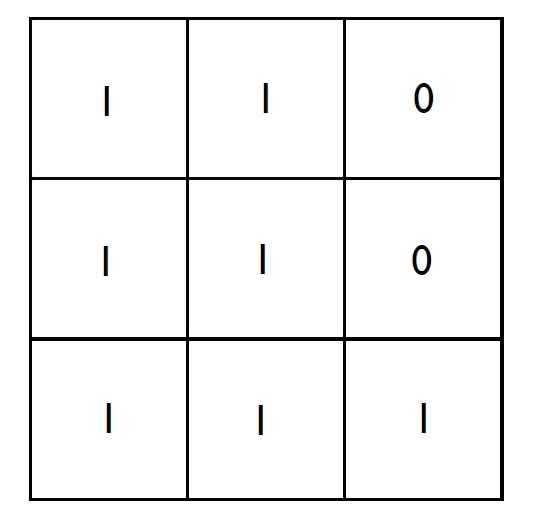
\includegraphics[width=0.5\linewidth]{tile0.jpg}
  \caption*{Initial dataset}
  \endminipage
  \minipage{0.30\textwidth}
  \centering
  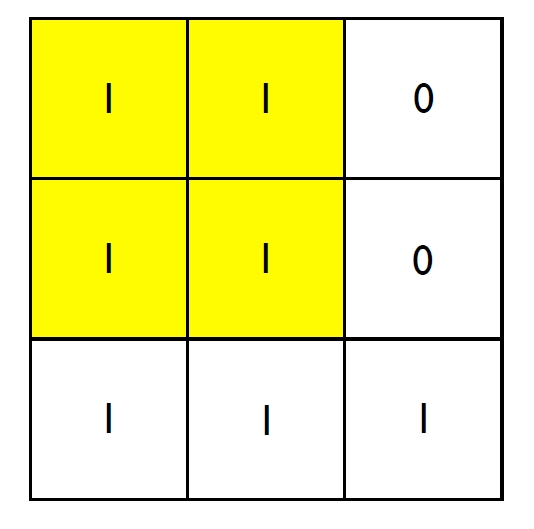
\includegraphics[width=0.5\linewidth]{tile2.jpg}
  \caption*{First tile}
  \endminipage
  \minipage{0.30\textwidth}%
  \centering
  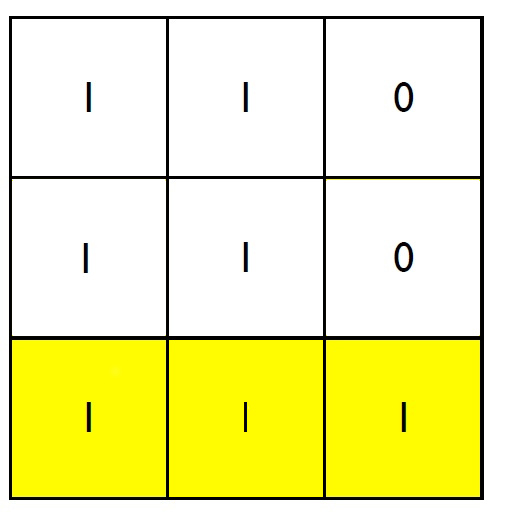
\includegraphics[width=0.5\linewidth]{tile1.jpg}
  \caption*{Second tile}
  \endminipage
  \caption{Example of Boolean tiles and their coverage}
  \label{tilesExample}
\end{figure}



\begin{definition}[Maximum $k$-Tiling]
Given a binary dataset $D$ and a positive integer $k$, find a tiling \bigT consisting of at most $k$ tiles and maximizing $\textit{area}(\bigT, D)$.
\end{definition}

We now formalize tiling as a relational data factorization problem and then solve it using ASP. Rather than restricting ourselves to Boolean values as in the traditional formulation, we consider the relational case. The standard way of dealing with tables in attribute-value datasets was to expand them into a sparse Boolean matrix (with one Boolean for every attribute-value). In contrast, our formulation employs the attribute-value format directly. 

%This also allows us to account for the {\tt car} example of Section \ref{decompositionExampleFigure}.

Given a relation \dbvars, denoting that transaction \transaction has \letter for \column, the task is to find a set of tiles that can be applied to the transactions to summarize the dataset \db. Here, a tile is a set of attribute-value pairs.

\begin{figure}[tbh]
	\centering
	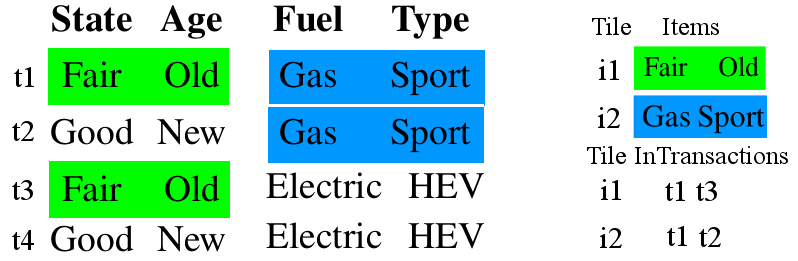
\includegraphics[width=.65\textwidth]{visualTiles.png}
	\caption{Relational tiling: two relational tiles (right) in a toy dataset (left) concerning cars.}
	\label{decompositionExampleFigure}
\end{figure}

In Figure \ref{decompositionExampleFigure}, for example, we can see the initial dataset, in which \textit{State} is an attribute and \textit{Fair} and \textit{Good} are values for this attribute.  Moreover, the blue and green areas indicate two relational tiles occurring in particular sets of transactions.

The two example tiles can be expressed as
\begin{align*}
   &\code(i_1,\textit{fair}, \textit{state}).~\code(i_1,\textit{old}, \textit{age}). ~\inrel(i_1,t_1). ~\inrel(i_1,t_3).\\
   &\code(i_2,\textit{gas}, \textit{fuel}).~\code(i_2,\textit{sport}, \textit{type}). ~\inrel(i_2,t_1). ~\inrel(i_2,t_2).
\end{align*}
where the first argument of each \code is the index of the tile, the second is the value of the attribute, and the third argument is the name of the attribute.
When tile $I$ is applied to a transaction $T$ (i.e., it occurs in the transaction), this is denoted by $\inrel(I,T)$. We call a set of tiles a \textit{tiling}.

We would like to factorize the initial dataset, 
represented as a set of $\db(\textit{fair}$, $\textit{state}, t_1)$, $\db(\textit{old},\textit{age},t_1)$, $\dots$,
using the following \textit{shape} query:
\begin{equation}
  \appr(\column,\letter,\transaction) \leftarrow \code(\indexvar,\letter, \column), \inrel(\indexvar,\transaction). %\text{~\footnotemark}
  \label{tilingshape}
\end{equation}
To reason about the coverage of the shape, i.e., which transactions and attributes are covered in the dataset (indicated by color in Figure \ref{decompositionExampleFigure}), we use the following definition: 
\begin{equation*}
  \covered( \transaction,\column) \leftarrow \appr(\column,\letter,\transaction). %\label{coverapprox}
\end{equation*}
For instance, $\covered(t_1,\textit{age})$ holds because $\code(i_1,\textit{old},\textit{age})$ and $\inrel(i_1,t_1)$ hold. 

To specify the maximum k-tiling problem, we need the following constraints.
\begin{description}
  \item[\onevalueConstraint:] for every attribute of a tile there is at most one value:
\begin{equation}
  \leftarrow \code(\indexvar,\textit{Val}_1, \column),\code(\indexvar,\textit{Val}_2, \column),\textit{Val}_1\neq \textit{Val}_2.  \label{def:tiling_conjunctive} 
\end{equation}
\item[\intersectionConstraint:] tiles do not overlap in the same transaction %(this constraint mimics LCM-$k$ behaviour \cite{tiling}, which only lets new tiles to only work on the uncovered area):
\begin{equation}
\leftarrow \inrel(I_1,T), \inrel(I_2,T), \code(I_1,V,A), \code(I_2,V,A), I_1 \neq I_2. \label{def:non_intersect} 
\end{equation}
  \item[\overcoverageConstraint:] tiles cannot ``overcover'' the transaction, that is, they are only allowed to cover tuples that are in the dataset;   
\begin{equation}
\leftarrow  \code(\indexvar,\letter, \column),\inrel(\indexvar,\transaction), \textit{not } \db(\letter, \column, \transaction). \label{def:pure_tiling}
\end{equation}
\item[\ktiles:] there are at most $k$-tiles (numbered from 1 to $k$): 
\begin{equation*}
   \indexvar = 1 \vee \indexvar = 2 \vee \dots \indexvar = k \leftarrow \code(\indexvar,\letter, \column).%  \label{eq:fixed_tiling}
\end{equation*}
\end{description}
Furthermore, the maximum k-tiling problem searches for the k tiles that maximize the area. This leads to an instance of the $\opti$ score defined by
  \begin{equation}
\maxcover: \quad \#\{ (T,A) : \covered(T,A) \}.  \label{eqn:coverage-opt} 
  \end{equation}
  The statement above correspond to the standard mathematical function optimization notation, that reads as follows: count (\#) the cardinality of the set ($\{ \cdot \}$) of tuples $(T,A)$ such that ($:$) $\covered(T,A)$ holds. When we translate this statements into ASP formulation we have to use special syntax of ASP (\textit{\#maximize}) to capture this mathematical formulation.
 
We specify the high-level model for maximum $k$-tiling in Listing \ref{lst:maxtiling:model}.
\begin{lstlisting}[style=model,label=lst:maxtiling:model,caption=Maximum $k$-Tiling ReDF Model]
 @\textbf{Input:}@ dataset @\db@and constant @$K$@
 @\textbf{Shape:}@ @$\appr(\column,\letter,\transaction) \leftarrow \code(\indexvar,\letter, \column), \inrel(\indexvar,\transaction)$@
 @\textbf{Find:}@  the set of ground facts @$\code(\cdot), \inrel(\cdot)$@
 @\textbf{Satisfying:}@@$\intersectionConstraint  \wedge \overcoverageConstraint$@
         @$\wedge~\ktiles \wedge \onevalueConstraint$@
@\textbf{Maximizing:}@ @\maxcover@ @\vspace{-1pt}
 \end{lstlisting}
To illustrate the advantages of our declarative and modular approach, let us consider a small variation of the tiling task, in which tiles may overlap. 
\paragraph{Overlapping tiling}
\begin{figure}[thb]
  \begin{center}
  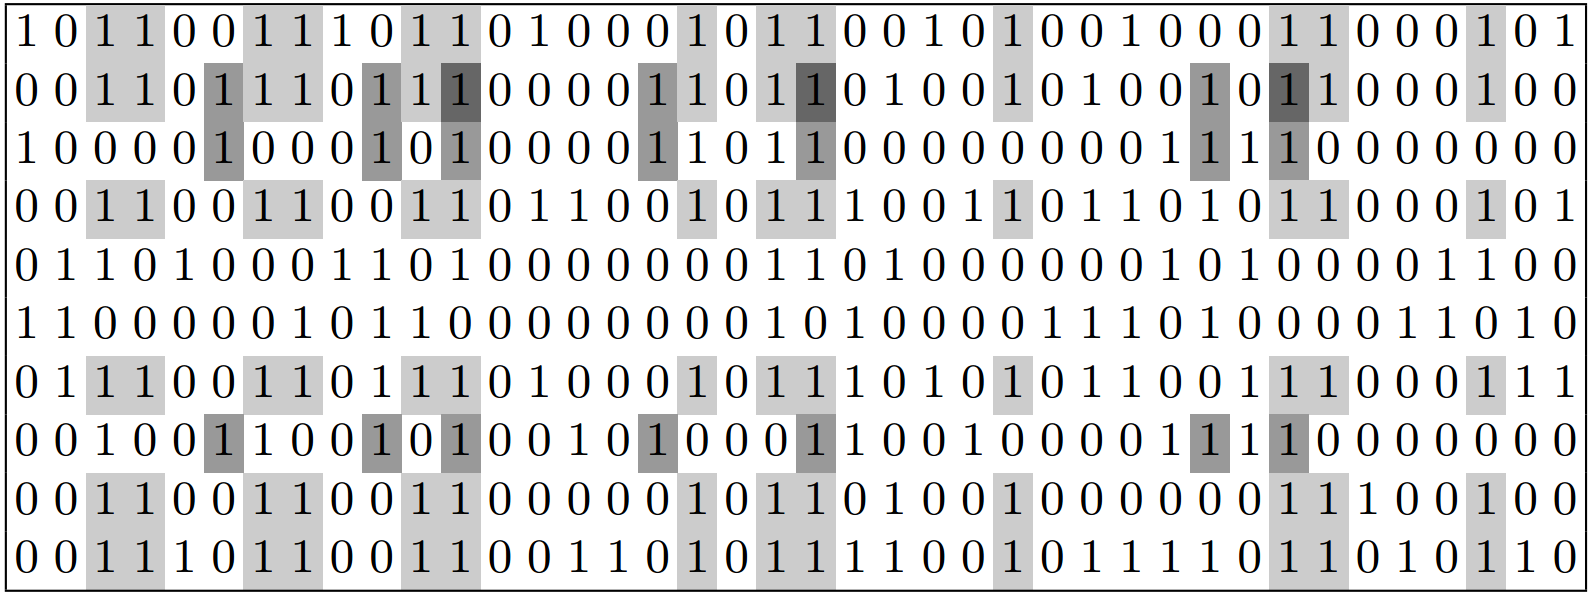
\includegraphics[width=.8\textwidth]{overlapping_geerts.png}
  \caption{Example of a 0/1 database with a tiling consisting of two overlapping tiles\\
  (darkest shaded area corresponds to the intersection of the two tiles), due to \cite{tiling}}
  \label{fig:geerts_overlapping}
\end{center}
\end{figure}
\label{subsubsec:overlapping_tiling}
Figure \ref{fig:geerts_overlapping}, taken from \cite{tiling}, illustrates a Boolean dataset with two overlapping tiles. We investigate and present two new variations of maximum $k$-tiling: overlapping and noisy tiling. The first investigates the global pattern mining task, when the overall coverage is optimized, allowing overlaps between tiles. The second investigates the task when, in $k$-maximum tiling, a tile can have a number of mismatches as covering a transaction. It is straightforward to change the assumption in our ReDF framework (and the corresponding ASP implementation). For the first task, it only involves replacing the constraint \intersectionConstraint by the following constraint.
\begin{description}
\item[\overlappingTilesConstraint:] two tiles in one transaction can intersect only on at most $N$ attributes:
\begin{equation*}
\leftarrow  \inrel(I_1,T), \inrel(I_2,T), \code(I_1,V,A_1), \code(I_2,V,A_2), I_1 \neq I_2, \# \{  A_1 = A_2\} > N.
\end{equation*}
\end{description}
To model the variation that tolerates some noise in the data, we can replace  constraint \overcoverageConstraint by 
\begin{description}
\item[\noiseConstraint:] every tile $I$ can overcover at most \textit{N} attributes in every transaction $T$ where it occurs: %In the algebraic formulation, it would change the \overcoverageConstraint to \noiseConstraint.
\begin{equation*}
\leftarrow  \code(I,V,A),\inrel(I,T), \textit{not}~ \db(V, A, T), \# \{ A \} > \textit{N}.
\end{equation*}
\end{description}
Both variations show that a slight change of the formulation of property of a solution leads to a small change in the modeling and to a small change in the implementation. 

\subsection{The Discrete Basis Problem (DBP) and Boolean Matrix Factorization (BMF)}
\label{subsection:bmf}
BMF has been extensively studied by \cite{conf/icdm/Miettinen12}, resulting in the well-known ASSO algorithm. Let us now show how it can be expressed as ReDF problem. As a starting point we take the same shape (Eq. \ref{tilingshape}) as in the tiling example in Subsection \ref{subsection:tiling}. However, we need to change the constraints to reflect the different properties of the desired solutions: tiles may now overlap, since one is not interested in tiles per se, but in good coverage of the dataset. That is why we remove 
the \intersectionConstraint and \overcoverageConstraint constraints, and introduce a notion of `overcoverage' instead, by means of the following definition:
\begin{equation*}
\overcovered(T,A) \leftarrow  \appr(V,A,T), \textit{not}~ \db(V,A,T). % \rightarrow \textit{overcovered}(T,A). 
\end{equation*}

In the Discrete Basis Problem, the scoring function maximizes the number of covered elements, while minimizing the overcovered ones. The latter term can be simply defined as: 
\begin{description}
\item[\overcoverage:] $\#\{ (T,A) : \overcovered(T,A) \}. $
\end{description}
We specify the high-level DBP model in Listing \ref{dbp:model:full}.
\begin{lstlisting}[style=model, caption=ReDF Model for the Discrete Basis Problem, label=dbp:model:full]
@\textbf{Input:}@ dataset @\db@and constants @$K,\alpha$@
@\textbf{Shape:}@ @$\appr(\column,\transaction) \leftarrow \code(\indexvar,\column), \inrel(\indexvar,\transaction)$@
@\textbf{Find:}@  the set of ground facts @$\code(\cdot), \inrel(\cdot)$@
@\textbf{Satisfying:}@ @$\ktiles$@
@\textbf{Maximizing:}@ @$\maxcover  - \alpha \times \overcover$@
\end{lstlisting}
This formulation mimics \textit{The Discrete Basis Problem} \citep{dbp}. That is, $K$ plays the role of the basis size and $\alpha$ mimics the bias towards rewarding covering and penalizing overcovering (the flags \texttt{--bonus-covered} and\\\texttt{--penalty-overcovered} in ASSO).
%The correspondence between these two formulations is explained in \ref{subsection:bmf_explanation}.

%Let us reformulate the problem in high algebraic language we used before (assuming the query is the same) \begin{align} & \onevalueConstraint \\ & \ktiles \end{align} Then, the optimization criterion takes into account overcoverage \begin{align} & \opti(M) = \coverage - \overcoverage \end{align}

It is well-known that tiling and {\em Boolean matrix factorization} (BMF) are closely related \citep{conf/icdm/Miettinen12}. Hence, let us also briefly show how BMF can be realized in our framework.  It corresponds to an instance of DBP where only binary values (true and false) are possible and the \overcoverageConstraint constraint applies. Hence, it is required that the factorization undercovers the initial dataset, i.e., if there is a 0 in a position in the original dataset, then there cannot be a 1 in the approximation.  Therefore, the optimization criterion of DBP is further simplified and we obtain the following BMF model, without overcovering, in Listing \ref{bmf:simplified:model}.
\begin{lstlisting}[style=model, label=bmf:simplified:model, caption=BMF without overcovering]
 @\textbf{Input:}@ dataset @\db@and constant @$K$@
 @\textbf{Shape:}@ @$\appr(\column,\transaction) \leftarrow \code(\indexvar,\column), \inrel(\indexvar,\transaction)$@
 @\textbf{Find:}@  the set of ground facts @$\code(\cdot), \inrel(\cdot)$@
 @\textbf{Satisfying:}@ @$\ktiles \wedge \overcoverageConstraint$@
 @\textbf{Maximizing:}@ @$\maxcover$@ @\vspace{-9pt}@
 \end{lstlisting}


\subsection{Discriminative k-pattern set mining}
\label{subsec:discriminative}
A common supervised data mining task is that of discriminative pattern set mining \citep{DBLP:conf/pkdd/KnobbeH06}.  Let \dbvars be a categorical dataset, \positiveT (\negativeT) be the set of positive (negative) transactions, and $ k$ the number of tiles. Then, the task is to find extensions of the relations \codevars and \invars such that positive and negative transactions are discriminated. A standard interpretation is to find tiles that cover as many positive and as few negative ones as possible \citep{Liu98integratingclassification}. The only required change in the model concerns the scoring function (and assigning some weight to the errors):
\begin{equation}
  \#\{T: \covered(T),\positiveT \} - \alpha \#\{ T: \covered(T),\negativeT \}, \label{eq:discriminate_optimization}
\end{equation}
where $\alpha$ is a constant that represents the weights for the errors made. It is typically a domain specific parameter (the cost of covering a negative example by a rule, i.e., the false
positive cost or a weight of a negative example).
Let us denote the coverage of the positive transactions as \coverageplus (left set term in Eq. \ref{eq:discriminate_optimization}) and the coverage of negative as \coverageminus (right set term in Eq. \ref{eq:discriminate_optimization}).  

Given that we have no \overcoverageConstraint constraint and negative transactions can be covered, the optimization criterion is given by
\begin{align*}
  & \opti(T) = \coverage^+ - \alpha \times \coverage^- .
\end{align*}

This corresponds to the high-level model in Listing \ref{lst:discriminative:model}.
\begin{lstlisting}[style=model,label=lst:discriminative:model,caption=ReDF Discriminative Patter Set Mining Model]
 @\textbf{Input:}@ dataset @\db@and constants @$K, \alpha$@
 @\textbf{Shape:}@ @$\appr(\column,\letter,\transaction) \leftarrow \code(\indexvar,\letter, \column), \inrel(\indexvar,\transaction)$@
 @\textbf{Find:}@  the set of ground facts @$\code(\cdot), \inrel(\cdot)$@
 @\textbf{Satisfying:}@ @$\ktiles \wedge \overcoverageConstraint \wedge \onevalueConstraint$@
 @\textbf{Maximizing:}@ @$\coverageplus - \alpha \times\coverageminus$@
\end{lstlisting}
\subsection{Block-diagonal matrix form}\label{subsec:blockdiagonal}
\begin{figure}[t]
\begin{center}
\begin{subfigure}{.32\textwidth}
  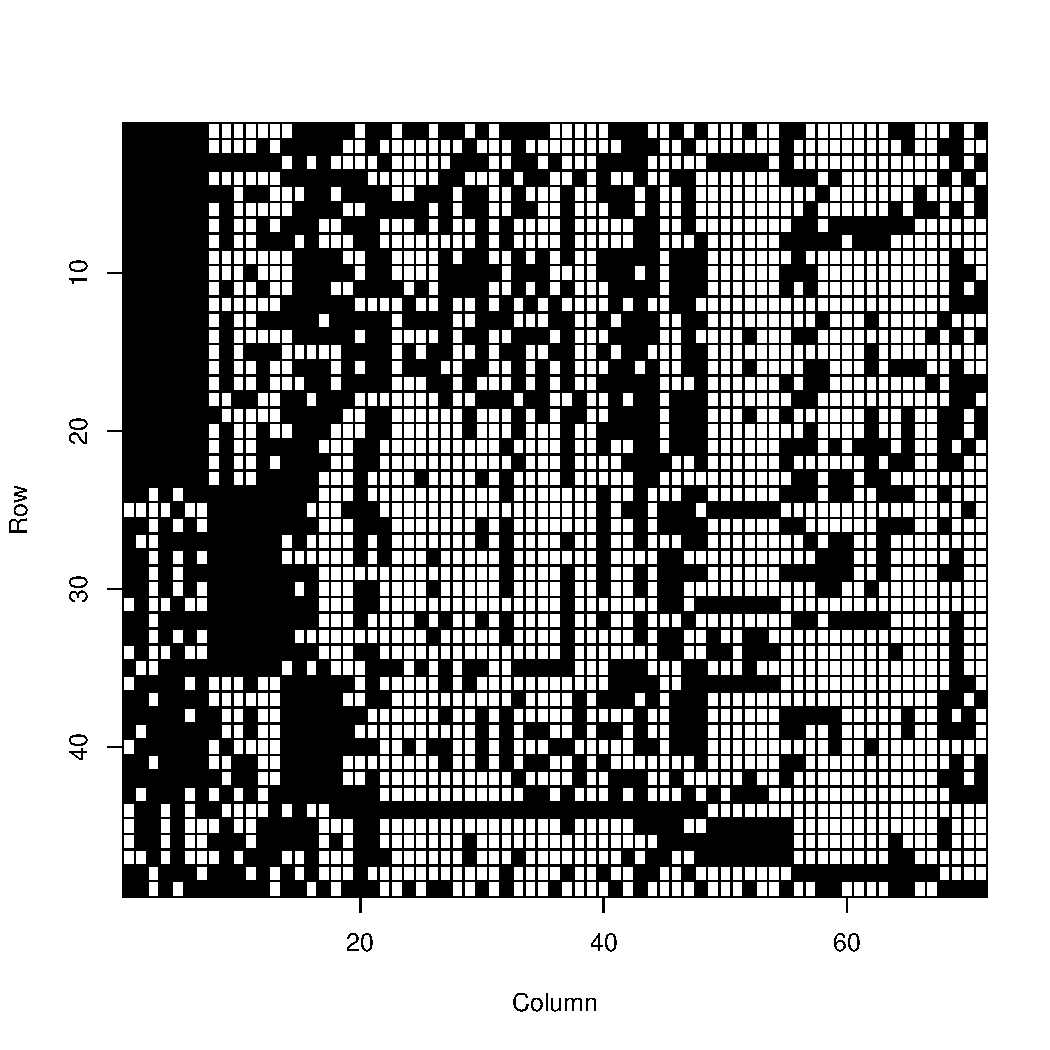
\includegraphics[width=\textwidth]{diagPure.pdf}
  \captionsetup{skip=-5pt}
  \caption{Regular}
  \label{fig:regular_block_diagonal}
\end{subfigure}
   \hfill 
\begin{subfigure}{.32\textwidth}
  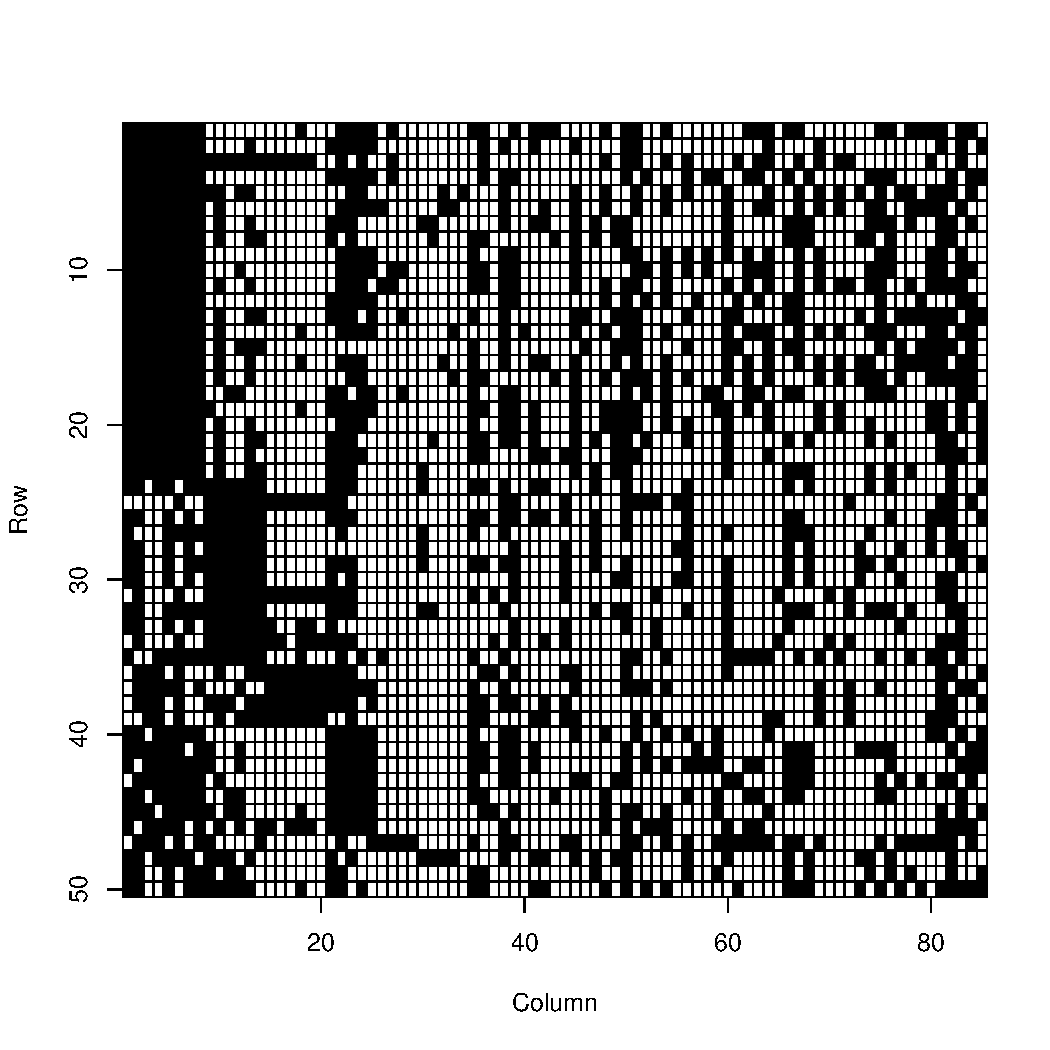
\includegraphics[width=\textwidth]{diagPenalty.pdf}
  \captionsetup{skip=-5pt}
  \caption{With penalties}
  \label{fig:penalty_block_diagonal}
\end{subfigure}
\begin{subfigure}{.32\textwidth}
  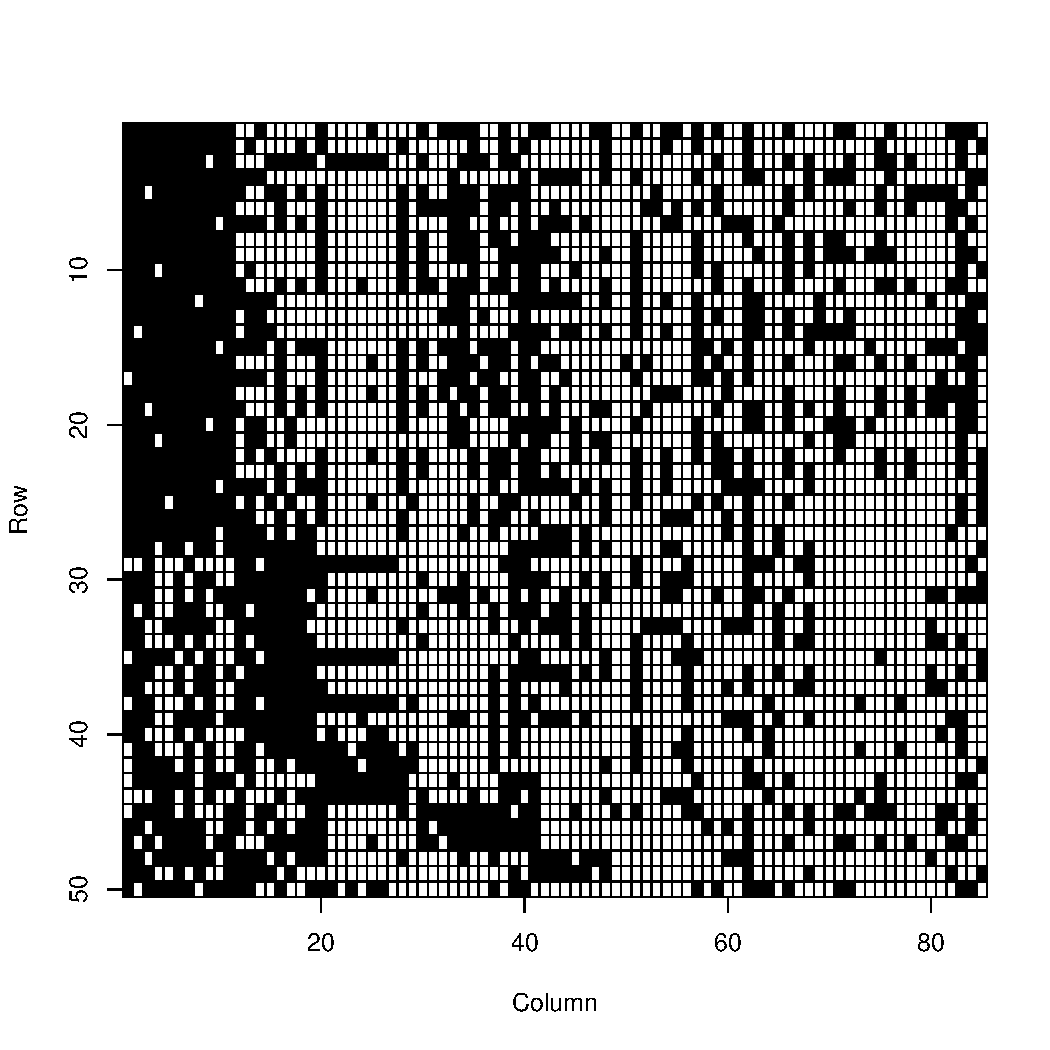
\includegraphics[width=\textwidth]{diagNoisy.pdf}
  \captionsetup{skip=-5pt}
  \caption{With penalties and noise}
  \label{fig:noisy_block_diagonal}
\end{subfigure}
\end{center}
\captionsetup{skip=-8pt}
\caption{Re-arranging a matrix in block-diagonal form (Animals dataset): (a) regular, (b) with penalties, (c) with noisy blocks and penalties}
\label{fig:diag_examples}
\end{figure}

\citet{blockdiagonal} introduced the problem of and an algorithm for permuting the rows and columns of a sparse matrix into block diagonal form. 
They relate this problem to other combinatorial and classical linear algebra problems. The underlying block-diagonal structure of a matrix can be used to parallelize certain matrix computations. An illustration of block-diagonalization (several variants) of the Animals dataset is depicted in Figure \ref{fig:diag_examples}.

We reduce it to a form of tiling. The shape query is the same as in tiling but the constraints are different: if a tile $I_1$ has an attribute $A$, then a tile $I_2$ cannot use the same attribute. A similar constraint is imposed on the $\inrel$ predicate and transactions stating that each item $A$ can belong to only one tile
\begin{description}
\item[\blockedItems:] $\leftarrow \code(I_1,A), \code(I_2,A), I_1 \neq I_2. $
\end{description}
Only one tile can occur in a transaction $T$.
\begin{description}
\item[\blockedTranst:] $\leftarrow  \inrel(I_1,T), \inrel(I_2,T), I_1 \neq I_2. $
\end{description}

We also modify the optimization criterion to take into account elements not covered by a tile but blocked by this tile. Every tile that selects attributes and transactions prohibits other tiles to use these attributes and transactions by means of the \blockedItems and \blockedTranst constraints. We penalize excessive usage of attributes and transactions by a single tile. We do this to improve the block form of the matrix, since in this task we are not just interested in a tiling with maximal coverage, but in a tiling that maximizes the number of elements on the diagonal and minimizes the number of elements everywhere else. To enforce this we introduce two functions:

\begin{description}
\item[\itemPenalty:] $\#\{ (T,A) : \appr(T,A'), ~\textit{not } \covered(T,A) \}$
\end{description}

\begin{description}
\item[\transactionPenalty:] $\#\{ (T,A) : \appr(T',A), ~\textit{not } \covered(T,A) \}$
\end{description}

Then, the whole problem is formulated in Listing \ref{lst:blockdiagonal:model}.
\begin{lstlisting}[style=model, label=lst:blockdiagonal:model, caption=ReDF Block-Diagonal Model]
@\textbf{Input:}@ dataset @\db@and constants @$N,\alpha,\beta$@
@\textbf{Shape:}@ @$\appr(\column,\letter,\transaction) \leftarrow \code(\indexvar,\letter, \column), \inrel(\indexvar,\transaction)$@
@\textbf{Find:}@  the set of ground facts @$\code(\cdot), \inrel(\cdot)$@
@\textbf{Satisfying:}@ @$\blockedTranst \wedge \blockedItems $@
              @$\onevalueConstraint \wedge \noiseConstraint \wedge \intersectionConstraint$@
@\textbf{Maximizing:}@ @$\coverage -\alpha \times \transactionPenalty - \beta \times \itemPenalty$@
\end{lstlisting}


If we omit \itemPenalty and \transactionPenalty, we obtain the standard optimization function for tiling. In the experimental section we evaluate the effect of the presence of this penalty. 




\section{Beyond classic problems}
\label{subsection:beoynd}
\label{sec:pure_decomposition}
% In this subsection we are going to talk about problems that lie outside of the scope normally discussed in the literature. 

% So far we have treated relations in the matrix-like manner, but it is easy to image a purely relational scenario where one can keep relational representation. Let us present a syntactic example that would mimic a possible real-world problem.  

So far we have focused on matrix-like representations of the data, in which the dataset was represented by instances of $\db(T,A,V)$, for a transactions $T$ having a value $V$ for an attribute $A$. This representation is independent of the number of attributes and values, it allows one to easily specify constraints over all attributes and to access the data using the predicate \db only.
%Using this representation one can express many data mining problems in a natural way, as shown in the previous section. 
We will now show that it is also possible to use other, purely relational representations, such as the {\em sells} example from the Introduction.

Section \ref{section:framework} already provided the {\em sells} example for decomposing 
a ternary relation into three binary ones.   In the shape for the {\em sells} example in Listing \ref{lst:sells}
%From database theory we know that a ternary relation $p(X,Y,Z)$ cannot always be factorized exactly into three binary relations \parencite{ternary_decomposition}.  But we may want to \emph{approximate} the ternary relation using ReDF. Assume that we have a relation \textit{\db(Author, University, Venue)}. Then we define the shape and the optimization criteria as \begin{align} &\textit{\appr(A,U,V)} \leftarrow \textit{worksAt(A,U), publishesAt(A,V), knownAt(U,V)}. \label{eq:pure_triple} \\ &\incorrect(A,U,V)   \leftarrow \db(A,U,V), \textit{not } \appr(A,U,V).\label{eq:incorrect1}\\ &\incorrect(A,U,V)   \leftarrow  \textit{not } \db(A,U,V),\appr(A,U,V).\label{eq:incorrect2}\\ &\texttt{incorrect}: \#\{(A,U,V):\incorrect(A,U,V)\}.  \label{eq:incorrect:minimize} \end{align}
there is no latent variable: there are only attributes from the original dataset. 
Since there is no latent variable, there is no ``pattern'' to be found for which the optimization criterion needs to be optimized, 
which allowed us to use a simple error function using only one type of atom. 

%That is, the body of \appr does not have latent variables and the whole model can be optimized simultaneously. This allowed us to have a simple optimization criterion
%that used only one type of atom.
%In this model we neither specified a bias towards covering, nor a penalty towards overcovering. This allows us to simplify the optimization criterion by using only one type of atoms.
%Further details will be discussed in Section \ref{section:implementation}.\\ \begin{lstlisting}[style=model,caption=Pure relational factorization, label=problem:pure_decomposition] @\textbf{Input:}@ dataset @\db@ @\textbf{Find:}@  the set of ground facts @$\textit{worksAt}(\cdot), \textit{publishesAt}(\cdot), \textit{knownAt}(\cdot)$@ @\textbf{Compute:}@ @$\textit{\appr(A,U,V)} \leftarrow \textit{worksAt(A,U), publishesAt(A,V), knownAt(U,V)}$@ @\textbf{Minimizing:}@ @\texttt{incorrect}@ \end{lstlisting}

However, latent variables can also be useful in a purely relational setting.
Let us illustrate this on an example inspired by the ArXiv community analysis example of \cite{Gopalan2013Efficient}. 
Assume we are given a relation \textit{publishedIn} with attributes \textit{Author}, \textit{University}, and \textit{Venue},
specifying that an author belonging to a particular university publishes in a particular venue. Furthermore, assume we want to factorize this relation into 
the relation  \textit{\appr(A,U,V)} by introducing a latent attribute \textit{Topic}, denoted as $T$. 
%Assume, we are given a relation \textit{publishedIn(Author, Uni, Venue)}, for short \textit{p(A,U,V)} and we would like to decompose it into the relation \textit{dp(A,U,V)} (short for decomposed-publishedIn) using the following shape: 
The latent topic variable clusters authors, universities and venues together in such a way that their join results in publications. 


We obtain the following high-level model in Listing \ref{lst:ternary:model}, 
where $\alpha$ is the constant that indicates the relative cost of overcovering an element and the integer constant $k$ is the number of value that the latent variable ($T$) can take:
\begin{align*}
& \appr(A,U,V) \leftarrow \textit{interestedIn}(A, \textit{T}), \textit{specializedIn}(U, \textit{T}), \textit{inField}(V, \textit{T}).
\end{align*}


\begin{lstlisting}[style=model,label=lst:ternary:model,caption=ReDF Purely Relational]
 @\textbf{Input:}@ dataset @\db and constants $K, \alpha$@
 @\textbf{Shape:}@ @$\appr(A,U,V) \leftarrow \textit{interestedIn}(A, \textit{T}), \textit{specializedIn}(U, \textit{T}), \textit{inField}(V, \textit{T}).$@
 @\textbf{Find:}@  the set of ground facts @$\textit{interestedIn}(\cdot), \textit{specializedIn}(\cdot), \textit{inField}(\cdot)$@
 @\textbf{Satisfying:}@ @$\ktiles$@
 @\textbf{Maximize:}@ @$\maxcover - \alpha \times \overcoverage$@
\end{lstlisting}
The corresponding model without latent variables would be different only in the decomposition shape, i.e., it would look like
\begin{equation*}
\appr(A,U,V) \leftarrow  \textit{worksAt(A,U), publishesAt(A,V), knownAt(U,V)}.
\end{equation*}

\paragraph{Discriminative relational learning}
In the spirit of discriminative pattern mining, described in Subsection \ref{subsec:discriminative}, we can also do discriminative learning in the purely relational setting. To do so, we assume that the relation has an extra argument Co-Author and we would like to discriminate the dataset by a particular Co-Author $c^+$, i.e., 
\begin{equation}
\begin{aligned}
 &\coverage^+(A,U,V) \leftarrow \appr(A,U,V), \textit{publishedIn}(A,U,V,c^+).\\
 &\coverage^-(A,U,V) \leftarrow \appr(A,U,V), \textit{publishedIn}(A,U,V,C), C \neq c^+.
\end{aligned} \label{eq:pure_relational_discriminative}
\end{equation}
Then, the optimization criterion remains the same as in Subsection \ref{subsec:discriminative}. Intuitively, if we have only information about an author of a paper (together with his or her university affiliation and a venue), we use this to `predict' his or her co-author using the patterns we obtain in this discriminative setting.

%The shape is somewhat reminiscent of statistical predicate invention as described in the work of \cite{predicateinvention}, 
%but is different in that we can use other optimization functions and constraints. 


% \subsection{Expressive pattern languages}
% \label{subsec:expressive_language}
% So far patterns were always conjunctions of attribute-value combinations, e.g., a tile in Figure \ref{decompositionExampleFigure} is a combination such as  
% \begin{equation*}
%   \textit{State} = \textit{fair}~\wedge~\textit{Age} = \textit{old}.
% \end{equation*}
% Our framework, however, can be easily adapted to also accommodate patterns such as 
% \begin{equation*}
%   (\textit{State} = \textit{fair} \vee \textit{State} = \textit{acceptable})~\wedge~\textit{Age} = \textit{old}.
% \end{equation*}
% This is known as \textit{internal disjunction} \parencite{internal_disjunction}. Conceptually, this would require changing constraint (\ref{def:tiling_conjunctive}) into a constraint 
% that allows up to $k$ values for the same attribute: 
% \begin{equation*}
% \leftarrow  \code(\indexvar,\letter_1, \textit{Attr}), \code(\indexvar,\letter_2, \textit{Attr}), \# \{ \letter_1 \neq \letter_2 \} \geq k.
% \end{equation*}

% A next step could be to support reasoning, e.g., about  a taxonomy of different values for the attributes. For instance, for the animal dataset \parencite{animalDataset} there could be a taxonomy about the types of animals specifying that  dog are carnivores, carnivores are mammals, etc. This would allow for tiles such as 
% \begin{equation*}
%   \textit{Class}~=~\textit{mammal} \wedge \textit{Birthtype}~=~\textit{egg-laying}.
% \end{equation*}
% If there is a platypus in the dataset, the system could deduce that it is a mammal and match it with the tile description. 
%  %a mammal), the system can deduce the fact that it is a mammal and it would match to the tile description. 
% This kind of reasoning is natural for logical reasoning systems like ASP and it is not hard to make an implementation using inference rules such as
% \begin{equation*}
%   \code(I,\textit{mammal}, \textit{class}) \leftarrow \code(I, \textit{dog}, \textit{class}).
% \end{equation*}
% %It say that for any pattern with an index $I$, if its class is equal to dog, then it also has the value mammal.

% In the same spirit as in \parencite{ebmf}, one could introduce negation into the pattern language with patterns such as
% \begin{equation*}
%   \textit{State} = \textit{fair}~\wedge~\textit{Age} \neq \textit{old}.
% \end{equation*}
% On the implementation level this requires introducing negated elements into possible values of an attribute, e.g., values of attribute \textit{birthtype} can be 
% \begin{equation*}
%   \{ \textit{egg-laying}, \textit{ovuliparity}, \textit{ovoviviparity}, \textit{not-egg-laying}, \textit{not-ovuliparity} \dots \}.
% \end{equation*}
% While at a conceptual level this coincides with internal disjunction, it results in a quite different search strategy. To see this we need to make the assumption that 
% the domains of the attributes are finite. If we allow $n-1$ values for an attribute among $n$ possible values, then it is the same as to prohibit only one $n$-th value, which would leave $n-1$ possible values.

% For the sake of clarity of presentation, in the current paper we refrain from experimenting with the expressive pattern languages discussed in this subsection.


\section{Implementation}
\label{section:implementation}
This section describes how ReDF models can be implemented in ASP. We do this for the basic problem of tiling, as well as for the purely relational data factorization presented before. Implementations of the other variations are included in Appendix \ref{ASP_appendix}. Our primary implementation is written in Clasp, can be used with the Clasp system \parencite{ASPbook,BrewkaCACM}.

\subsection{General computation methods: greedy and sampling approaches.} 
In all described problems, the goal is to find $k$ patterns or tiles, where a pattern is interpreted as a set of facts corresponding to a particular value of the latent variable. 
We will follow an iterative approach to finding these patterns,
in which the discovery of the next pattern or tile will be encoded in ASP.
We will consider both a {\em greedy} and a {\em sampling} algorithm
for realizing this. The sampling approach is intended for better scalability and will
be evaluated in Section \ref{subsec:experiments_tiling}.

\textit{Greedy model.}
The greedy approach is described  in  Algorithm \ref{alg:greedy}. Essentially, 
when the next best \tile has been computed (where \tile is a set of facts associated with the \tile identifier, e.g., in tiling a pattern is a set of transactions and attributes), it is added to the current set of \tiles. The specific part for each tile is represented by \texttt{executeProgram} and is encoded separately in ASP. Note that this greedy, iterative approach to finding $k$ patterns is very common in pattern mining. 
\changesb Theoretical bounds on the solution quality of the greedy approach have been studied in the context of the maximum $k$-set coverage problem \parencite{max_k_set_cover1, max_k_set_cover2}; more details can be found in Appendix \ref{appendix:k_set_coverage_analysis}. \changese
\begin{figure}[thb]
\captionof{algorithm}{Greedy execution model}
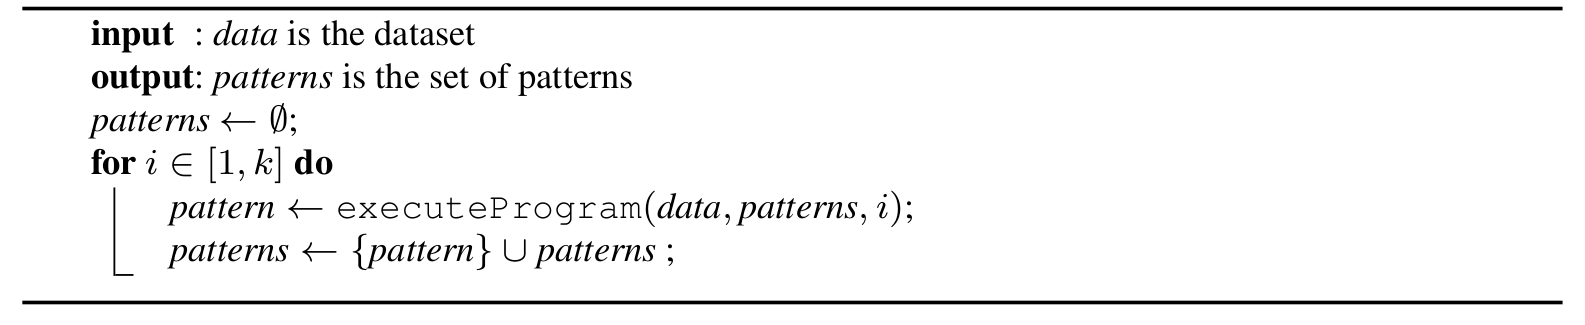
\includegraphics[width=\textwidth]{algorithm1_greedy.png}
 \label{alg:greedy}
\end{figure}

\textit{Column sampling execution model.} To improve scalability, we employ a sampling approach. Interestingly, our approach is different from most existing sampling techniques in data mining: instead of sampling a rows or patterns, we sample columns. Algorithm \ref{sampling} presents the column sampling approach we propose. The key difference with the greedy approach is that instead of determining the 
next best pattern on the {\em overall} dataset in each iteration, this approach samples $N$ subsets of the data
and determines the next best pattern for all of these subsets. The best among these is then fixed,
and the process is repeated. We empirically evaluate the effects of sampling
on the quality of the computed patterns and on the runtime in the experiment section. \changesb Quality bounds for this type of greedy search have also been analyzed previously \parencite{max_k_set_cover1}; for more details we refer to Appendix \ref{appendix:k_set_coverage_analysis}. \changese
\begin{figure}[thb]
\captionof{algorithm}{Column sampling execution model}
 \label{sampling}
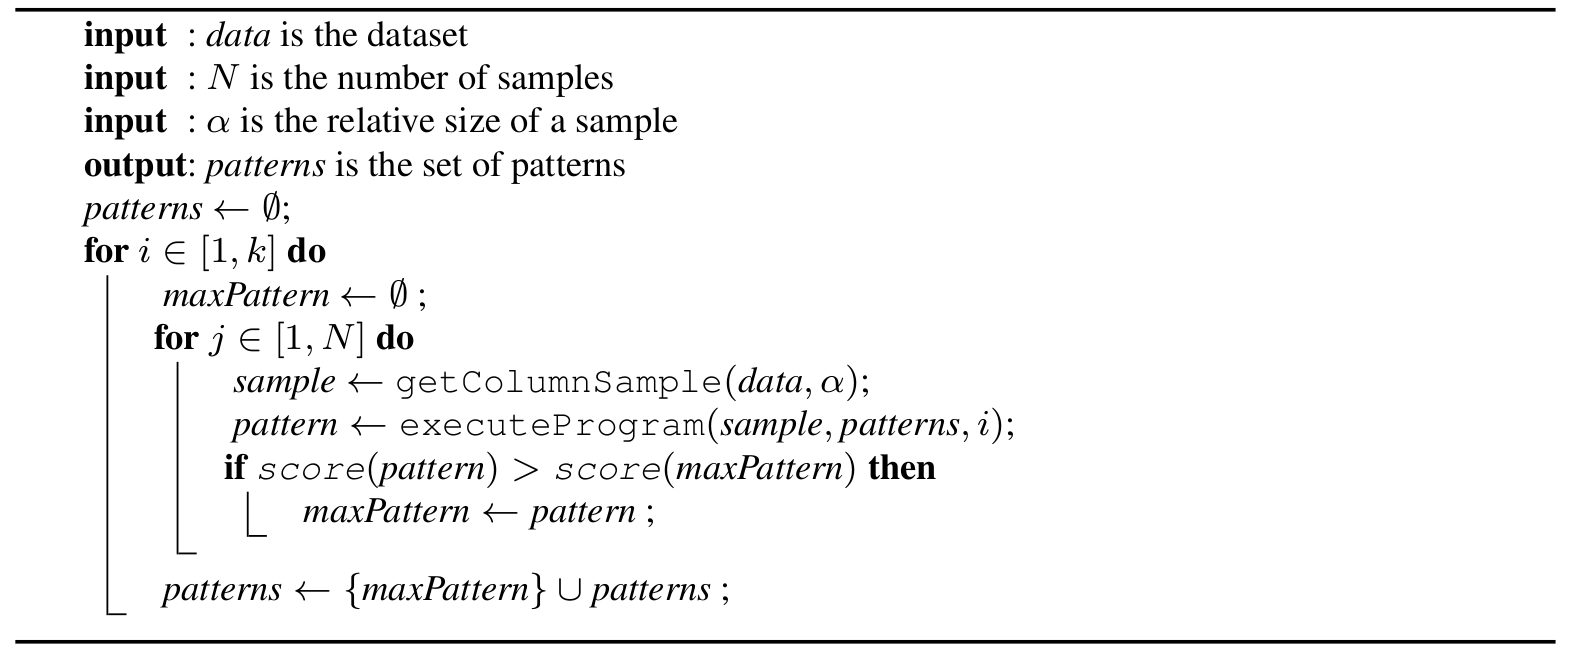
\includegraphics[width=\textwidth]{algorithm2_greedy_sampling.png}
\end{figure}

\lstset{numbers=left,
  numberstyle=\tiny,
  numbersep=5pt,
  basicstyle=\small,
  stringstyle=\sffamily,
  columns=fullflexible,
  flexiblecolumns=true,
  belowskip=5pt,
  alsoletter={-}, 
  alsodigit={:},
%  otherkeywords={},
  emph={%
      not,
      :-,
          },emphstyle={\bfseries}%
}
\begin{lstlisting}[float,floatplacement=t, caption=Greedy maximum $k$-tiling formalization in answer set programming, label=lst:encoding, escapeinside={@}{@}] 
@\commenttextasp{\%\onevalueConstraint; it generates at most one value per attribute}@
0 { tile(current, Value, Attribute) : valid(Attribute, Value) } 1 :- col(Attribute). @\label{guess_line}@
@\commenttextasp{\%\overcoverageConstraint}@
over_covered(current,T) :- not db(Val, Attr, T), tile(current, Val, Attr), transaction(T). @\label{overcover_line}@
@\commenttextasp{\%\intersectionConstraint}@
intersect(T) :- current != I, tile(current, Val, Attr), tile(I, Val, Attr), in(I,T). @\label{intersect_line}@
@\commenttextasp{\%defines presence of tiles in transactions}@
in(current,T) :- transaction(T), not over_covered(current, T), not intersect(T). @\label{in_line}@
@\commenttextasp{\%defines \maxcover function}@
covered(Transct, Attribute) :- in(Index,Transct), tile(Index, _, Attribute). @\label{covered_line}@
#maximize[covered(Transct, Attribute)]. @\label{maximize_line}@
\end{lstlisting}

\subsection{Data mining problems expressed in the framework} 

The maximum $k$-tiling problem can be encoded in answer set programming as indicated in Listing~\ref{lst:encoding}. The code implements the greedy model, i.e., Algorithm \ref{alg:greedy}, for the maximum $k$-tiling problem with a fixed number of tiles \parencite{tiling}. It assumes we have already found an optimal tiling for $n-1$ tiles, and indicates how to find the $n$-th tile to cover the largest area. The $n$-th tile is called \guess in the listing. \changesb Further, we have information about the names of the attributes and the possible values for each attribute through predicates $\col(\column)$ and $\valid(\column, \letter)$. That is, $\col(A)$ is an unary predicate that encodes possible column indices, and $\valid(A,V)$ is a binary predicate that encodes which possible values $V$ can occur in column $A$. \changese

Let us explain the code in Listing \ref{lst:encoding}. The constraint in Line \ref{guess_line} generates at most one value for each attribute. The constraints in Lines \ref{overcover_line} and \ref{intersect_line} compute the transactions where the current tile cannot occur, i.e., \texttt{intersect(T)} is the set of all transactions where the current tile overlaps with another tile and the current tile cannot cover these transactions. Similarly, \texttt{overcovered(currentI,T)} is the set of transactions that cannot be covered because there is an element in the current tile, with fixed index \texttt{currentI}, that is not present in transaction \texttt{T}. The constraint in Line \ref{in_line} states that if the tile does not violate the overcovering and intersection constraints in a transaction, it occurs in the transaction. Line \ref{covered_line} defines the coverage and the optimization constraint in Line \ref{maximize_line} enforces the selection of the best model.

\begin{theorem}[Correctness of the greedy ASP tiling encoding]\label{theorem:tiling}
 The ASP program \pprog defined by the Listing \ref{lst:encoding} computes the $k$-th largest tile w.r.t. the scoring function \maxcover (\ref{eqn:coverage-opt}) as extensions of the predicates $\code(k,\cdot,\cdot)$ and $\inrel(k,\cdot)$ in its answer set \as, provided that 
the dataset is represented extensionally through the predicates \db, \valid, and \col 
and the $k-1$ already found tiles are represented extensionally through the predicates $\code(I,\cdot,\cdot)$ and $\inrel(I,\cdot)$ for $I \in [1,k-1]$.
\end{theorem}
For the proof, see Appendix \ref{proof:tiling}.
The Clasp encodings for the other models are sketched in Appendix \ref{ASP_appendix}.

\subsection{Purely relational data factorization}
In Section \ref{sec:pure_decomposition} we presented a factorization of the \emph{publishedIn} relation into three binary relations. It constitutes a proof-of-concept prototype model in ASP and could be improved by, e.g., incorporating heuristics. %The proof of correctness is presented in Appendix \ref{sec:proof_pure_encoding}.
%\ref{lst:pure_alternative}

The general structure of the ASP encoding is similar to the \emph{sells} example in Listing \ref{lst:sells}: we indicate here only a possible optimization for the relation generators.  We use the left-to-right order of the atoms in the schema (replicated below) while generating candidates for the factorization.

% @\commenttextasp{\%factorization shape}@
% approx(A,U,V)      :- works_at(A,U), publishes_at(A,V), known_at(U,V). @\label{lst:pure:line:approx}@
% @\commenttextasp{\%relation generators}@
% @\commenttextasp{\%optimization function}@
% incorrect(A,U,V) :- approx(A,U,V), not p(A,U,V). @\label{lst:pure:incorrect1}@
% incorrect(A,U,V) :- not approx(A,U,V), p(A,U,V). @\label{lst:pure:incorrect2}@
% #minimize[incorrect(A,U,V)]. @\label{lst:pure:minimize}@
\begin{lstlisting}[caption=Generators for the model without a latent variable into three binary relations, escapeinside={@}{@}, label=lst:pure_alternative] 
0 { works_at(A,U)     } 1 :- published_in(A,U,V). @\label{lst:pure:gen1}@
0 { publishes_at(A,V) } 1 :- published_in(A,U,V), works_at(A,U). @\label{lst:pure:gen2}@
0 { known_at(U,V) } 1 :- published_in(A,U,V),works_at(A,U),publishes_at(A,V).@\label{lst:pure:gen3}@
\end{lstlisting}


\textit{Implementation differences.} When we generalize the factorization encoding with two relations to three relations, we observe a slight implementation difference between them. Factorization with the two relation shapes can be naturally implemented using the core ASP generate-and-test paradigm. Once we have guessed an extension for a certain value of the latent variable, we propagate it to the second relation and test against the constraints. This strategy is often deployed in specialized algorithms \parencite{tiling, dbp}.
For a multiple relation shape we guess an extension of one relation, then we constrain the possible values we generate for the second value (e.g., see Line \ref{lst:pure:gen2} in Listing \ref{lst:pure_alternative}). In general, we can search for one at a time using a greedy strategy (as in tiling). Theoretically, we can simultaneously search for values of a latent variable by replacing the fixed latent parameter by a variable and searching over the latent parameter as well. The work of \cite{tias_topk} provides evidence that this approach does not scale well, unless special propagators are introduced into the solver. This technique would allow extending the method to other shapes with more than three relations.


\section{Experiments}
\label{section:experiments}

\begin{table}[b]
% \captionsetup{   font = {scriptsize},  }
 \caption{Dataset properties. For each dataset,  we specify whether the attributes have Boolean or categorical domains, the number of tuples and attributes, and the average number of distinct values per attribute}
 \label{table:dataset_description}
%\scalebox{.9}{
\begin{tabular}{lcrrr}
\textbf{Dataset} & \textbf{Attributes} & \textbf{\# tuples} & \textbf{\# attributes} & \textbf{Avg \# values per attribute}  \\
Animals          & Boolean         &  $50$  &  $85$  &  2  \\
Solar flare      & categorical &  $1\,389$  &  $11$  &  $3.3$  \\
Tic-tac-toe      & categorical  &  $958$  &  $10$  &  $2.9$  \\
Nursery          & categorical &  $12\,960$  & $8$  &  $3.4$  \\
Voting           & categorical &  $435$  &  $17$  &  $3.0$  \\
Chess (Kr-vs-Kp) & categorical &  $3\,196$  &  $36$  &  $2.1$  \\ 
Mushroom         & categorical &  $8\,124$  &  $22$  &  $5.6$
\end{tabular}
%}
\end{table}

The main goal of this section is to evaluate whether ReDF problems can be solved using a generic solver. In particular, we focus on solving the problem formulations as we specified them in ASP. We investigate whether the problems can be solved, and for a number of tasks compare the results and runtimes to those obtained by specialized algorithms. Since we here use generic problem formulations and generic solvers that have neither been designed nor optimized for the tasks under consideration, we cannot expect the approach to be as efficient as specialized algorithms. However, what is more important is that we demonstrate that all tasks formalized and prototyped using the ReDF framework can be solved using a unified approach.


\textit{Experimental setup and datasets.} The ASP engine we use is 64-bit clingo (clasp with the gringo grounder) version 3.0.5 with the parameter \texttt{--heuristic=Vmtf} (see Appendix \ref{subsec:evaluatingsolver} for details on the parameters) and all experiments are executed on a 64-bit Ubuntu machine with Intel Core i5-3570 CPU @ 3.40GHz x 4 and 8GB memory, except for Maximum $k$-tiling on Chess and Mushrooms datasets where Intel Xeon CPU with 128GB of memory (all single-threaded) has been used due to high memory requirements. For most experiments we use the datasets summarized in Table \ref{table:dataset_description}, which all but one originate from the UCI Machine Learning repository \parencite{ucidatasets}. The \emph{Animals (with Attributes)} dataset was taken from \cite{animalDataset}. For the purely relational factorization task, the data and experiment results are described separately in the corresponding subsection. 

In Subsection~\ref{subsec:solvingexisting} we show how ReDF formulations of existing data mining tasks (from Section~\ref{section:dm_problems}) can be solved using the implementation presented in Section~\ref{section:implementation}, afterwards in Subsection~\ref{subsec:solvingrelational} we show the results of the purely relational data factorization task. The ASP solver parameters used in the experiments and a breakdown of individual solving steps and their runtimes determined by the meta-experiment are presented in Appendix~\ref{subsec:evaluatingsolver}.

\subsection{Solving existing tasks}
\label{subsec:solvingexisting}
\paragraph{Maximum $k$-Tiling in Categorical Data}
\begin{table}[t]
\captionsetup{
    font = {small},
  }
\begin{center}
\caption{Maximum $k$-Tiling}
\label{tab:tiling}
\begin{subtable}{.45\textwidth}
\captionsetup{
    font = {small},
  }
\caption{Runtime}
\label{tab:tiling:time}
\scalebox{.75}{
\begin{tabular}{lrrrrr}
  \phantom{Dataset} & \multicolumn{5}{c}{\textbf{Number of tiles ($k$)}}\\
\textbf{Dataset} & \textbf{5} &    \textbf{10} &   \textbf{15} &  \textbf{20} & \textbf{25} \\ \hline
Animals    &36s  & 1m4s  &  1m21s  &  1m32s  & 1m36s \\
Solar flare&6s   & 10s  &  13s  &  16s  & 18s \\
Tic-tac-toe&22s  & 31s  &  33s  &  34s   & 35s \\
Nursery    &4m19s & 6m32s &  7m32s &  7m56s & 8m13s \\
Voting     &52s  &  1m28s &  1m42s &  1m46s & 1m49s \\
Chess      &17h03m & 22h31m & - & - & -\\
Mushroom &13h09m & 19h44m & - & - & -\\
\end{tabular}
}
\end{subtable}
\hfill
\begin{subtable}{.41\textwidth}
\captionsetup{
    font = {small},
  }
\caption{Coverage}
\label{tab:tiling:coverage}
\scalebox{.75}{
\begin{tabular}{rrrrr}
  \multicolumn{5}{c}{\textbf{Number of tiles ($k$)}}\\
\textbf{5} &    \textbf{10} &   \textbf{15} &  \textbf{20} & \textbf{25} \\ \hline
0.327 & 0.472 & 0.573 & 0.649 & 0.709\\
0.416 & 0.565 & 0.655 & 0.721 & 0.751\\
0.251 & 0.449 & 0.623 & 0.784 & 0.907\\
0.269 & 0.454 & 0.634 & 0.773 & 0.905\\
0.399 & 0.553 & 0.662 & 0.749 & 0.810\\
0.483 & 0.618 &- &-   &-\\
0.476 & 0.586 &-   &- &-
\end{tabular}
}
\end{subtable}
\end{center}
\end{table}


\label{subsec:experiments_tiling}

We first consider the Maximum $k$-Tiling problem from Section \ref{subsection:tiling} and present timing and coverage results in Table~\ref{tab:tiling} obtained on all datasets from Table \ref{table:dataset_description}.

In all cases the problem specification given in Listing~\ref{lst:encoding} was used to greedily mine $k=25$ tiles. Since the problem becomes more constrained as the number of tiles increases, runtime decreases for each additional tile mined. We therefore report total runtime and coverage for different values of $k$, i.e., for different total numbers of tiles. Only $k=10$ tiles were mined on Chess and Mushroom due to long runtimes.


\textit{Effect of sampling~}As we can see from Table~\ref{tab:tiling:time}, runtimes are quite long on datasets like Mushroom. To address this issue, we use the sampling procedure of Algorithm~\ref{sampling} with the following parameters: $\alpha = 0.4$ and $N = 20$, i.e., 40\% of all attributes were selected uniformly at random for each sample and 20 samples were used. Intuitively, the larger the sample size and the more samples, the better we approximate the exact result.

With the given parameters, we attain an order of magnitude improvement in runtime: instead of 19 hours with the regular algorithm, using sampling it takes only one hour to compute 10 tiles as indicated in Figure \ref{fig:tiling_time_comparison}. The effect of using sampling on coverage can be seen in Figure~\ref{fig:tiling_comparison}: the first tiles that are mined have lower coverage than when sampling is not used, but after a while the difference in coverage with LTM-k remains more or less constant and even slightly decreases. LTM-k is the original, specialized tiling algorithm, to which we compare next.


\textit{Comparison to a specialized algorithm~}We now compare the performance of the ASP-based implementation of LTM-k greedy strategy to that of a specialized implementation\footnote{\url{http://people.mmci.uni-saarland.de/~jilles/prj/tiling/}}. Figures~\ref{fig:tiling_time_comparison} and~\ref{fig:tiling_comparison} present both runtime and coverage comparisons obtained on Mushroom, both for our approach (with and without sampling) and the specialized miner. 

Without sampling, we can see that our approach gives the same results in terms of the coverage as the LTM-k algorithm. This is as expected though, since both LTM-k and our approach guarantee to find an optimal solution in each iteration. \changesb The slight difference between the two coverage curves in Figure \ref{fig:tiling_comparison} is caused by the fact that multiple tiles can have the same (maximum) area, and some choice between those has to be made. Although these choices are typically made deterministically, the different implementations make decisions based on different criteria, resulting in slightly different tilings. \changese

Unfortunately, the ASP solver is not as efficient as the specialized miner as can be seen in Figure \ref{fig:tiling_time_comparison}, and the generality of the approach comes at the cost of longer runtimes. However, as already discussed, using a sampling approach can substantially decrease the runtime. Experiments on other datasets showed similar behavior to that depicted here.

\begin{figure}[t]
      \captionsetup{
                   skip=-2pt
                 }
  \begin{center}
    \begin{subfigure}{.49\textwidth}
      \captionsetup{
                   font={scriptsize},
                   skip=-5pt
                 }
      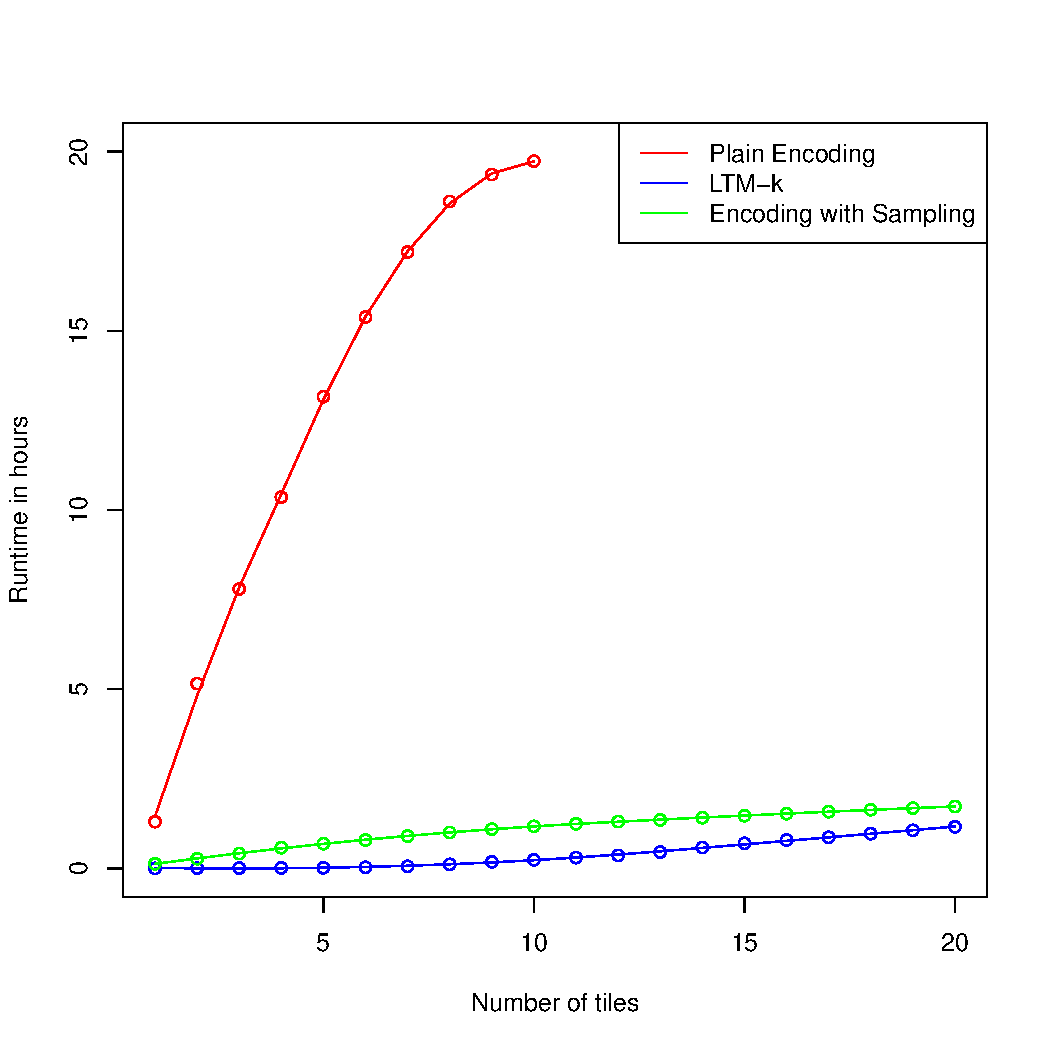
\includegraphics[width=\textwidth]{tiling-time-plot.pdf}
      \caption{Runtime}
      \label{fig:tiling_time_comparison}
    \end{subfigure}
    \hfill 
    \begin{subfigure}{.49\textwidth}
      \captionsetup{
                   font={scriptsize},
                   skip=-5pt
                 }
      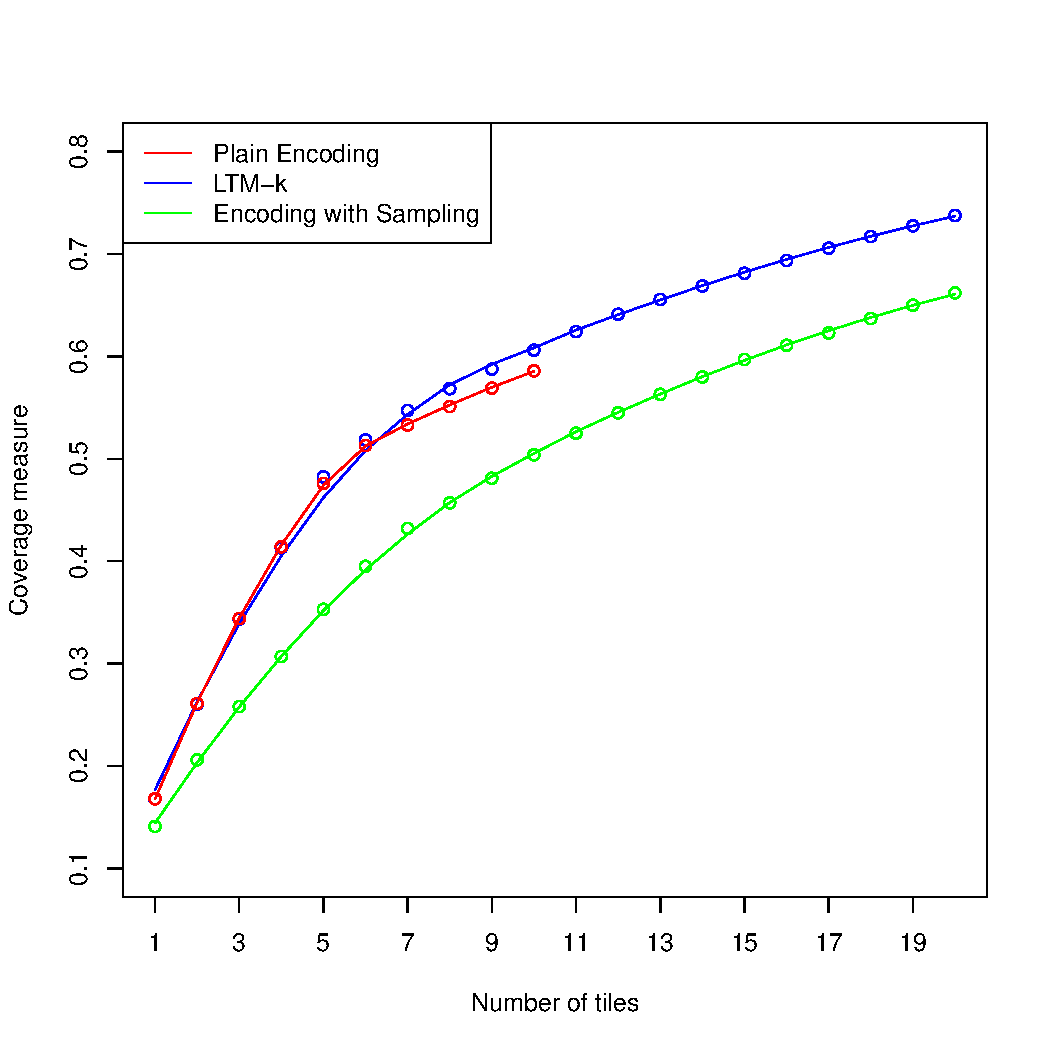
\includegraphics[width=\textwidth]{tiling_comparison.pdf}
      \caption{Coverage}
      \label{fig:tiling_comparison}
    \end{subfigure}
  \caption{Tiling comparison (runtime, coverage) with LTM-k (Mushroom dataset)}
  \end{center}
\end{figure}

\paragraph{Overlapping tiling}
To evaluate the overlapping tiling task from Subsection \ref{subsubsec:overlapping_tiling}, we apply the model in Listing~\ref{encoding_noisy} (ASP encoding in Appendix \ref{ASP_appendix}) to the five smaller datasets from Table \ref{table:dataset_description}. We experiment with two levels of overlap, i.e., parameter $N$ is set to either 1 or 2: tiles can intersect on at most one or two attribute(s). As the results in Table~\ref{tab:overlapping} show, allowing limited overlap can lead to a small increase in coverage, but runtimes also increase due to the costly aggregate operation in Line~\ref{line_intersect_count} of Listing~\ref{encoding_noisy}. 

However, what is important to emphasize here is that only a small change in the problem formalization is sufficient to allow for overlap in the tilings, while the solver can still solve the problem without any further changes. And although the runtimes are longer when more overlap is allowed, the difference with the basic, non-overlapping setting is moderate.

\begin{table}[t]
\captionsetup{
    font = {small},
  }
\begin{center}
\caption{Maximum $k$-Tiling with overlap. The maximal allowed overlap is limited by parameter $N$}
\label{tab:overlapping}
\begin{subtable}{.36\textwidth}
\caption{Runtime}
\label{tab:overlapping:time}
\scalebox{.75}{
\begin{tabular}{lcrrrrrr}
\phantom{Dataset}     & \multicolumn{5}{c}{\textbf{Number of tiles ($k$)}}\\
\textbf{Dataset}      &  \textbf{N} &  \textbf{5} &    \textbf{10} &   \textbf{15} &  \textbf{20} & \textbf{25} \\ \hline
Animals               & 1 & 1m10s &2m28s&3m46s&4m24s &4m47\\
\phantom{Animals}     & 2 & 1m39s &4m10s&6m26s  &7m40s&8m10s\\
Solar flare           & 1 & 8s  &13s &17s   &21s &24s\\
\phantom{Solar flare} & 2 & 8s  &15s &20s   &25s &29s\\
Tic-tac-toe           & 1 & 24s &41s &49s   &52s &53s\\
\phantom{Tic-tac-toe} & 2 & 23s &43s &51s   &55s &56s\\
Nursery               & 1 & 5m00s&8m19s&10m10s  &10m48s&11m12s\\
\phantom{Nursery}     & 2 & 5m43s&9m32s&11m9s&11m50s&12m12s\\
Voting                & 1 & 1m10s &2m19s& 2m53s &3m8s&3m15s\\
\phantom{Voting}      & 2 & 1m39s &3m34s& 4m35s &5m9s&5m33s
\end{tabular}
}
\end{subtable}
\hfill
\begin{subtable}{.37\textwidth}
\caption{Coverage}
\label{tab:overlapping:coverage}
\scalebox{.75}{
\begin{tabular}{rrrrr}
\multicolumn{5}{c}{\textbf{Number of tiles ($k$)}}\\
\textbf{5} &    \textbf{10} &   \textbf{15} &  \textbf{20} & \textbf{25} \\ \hline
0.327&0.475&0.583&0.663&0.722\\
0.332&0.482&0.592&0.675&0.742\\
0.433&0.595&0.684&0.734&0.756\\
0.452&0.602&0.685&0.731&0.755\\
0.253&0.451&0.626&0.781&0.898\\
0.253&0.451&0.626&0.781&0.898\\
0.268&0.454&0.633&0.772&0.905\\
0.268&0.454&0.633&0.772&0.905\\
0.403&0.558&0.675&0.765&0.828\\
0.409&0.571&0.683&0.762&0.819
\end{tabular}
}
\end{subtable}
\end{center}
\end{table}

\paragraph{Boolean matrix factorization (BMF)}
We perform Boolean matrix factorization (Section \ref{subsection:bmf}) by applying the formalization of Listing~\ref{bmf} and compare the results to those obtained by ASSO\footnote{\url{http://www.mpi-inf.mpg.de/~pmiettin/src/DBP-progs/}} \parencite{conf/icdm/Miettinen12} with the no-overcoverage flag (\texttt{-P1000}). The factorization rank $k$ is incremented by one in each iteration, and meanwhile coverage gain and runtime are measured. The results for Animals are presented in Figure~\ref{figure:bmf} and show that coverage is almost identical to that obtained by ASSO. Again, this is unsurprising, as our implementation follows the same solving strategy.  However, runtimes are several times higher, which is due to the usage of a general solver that is not optimized for this type of task. Results obtained on other datasets are very similar and are therefore not presented here.

\begin{figure}
%  \vspace{-3mm}
\begin{center}
\begin{subfigure}{.49\textwidth}
\centering
\captionsetup{skip=-3pt}
  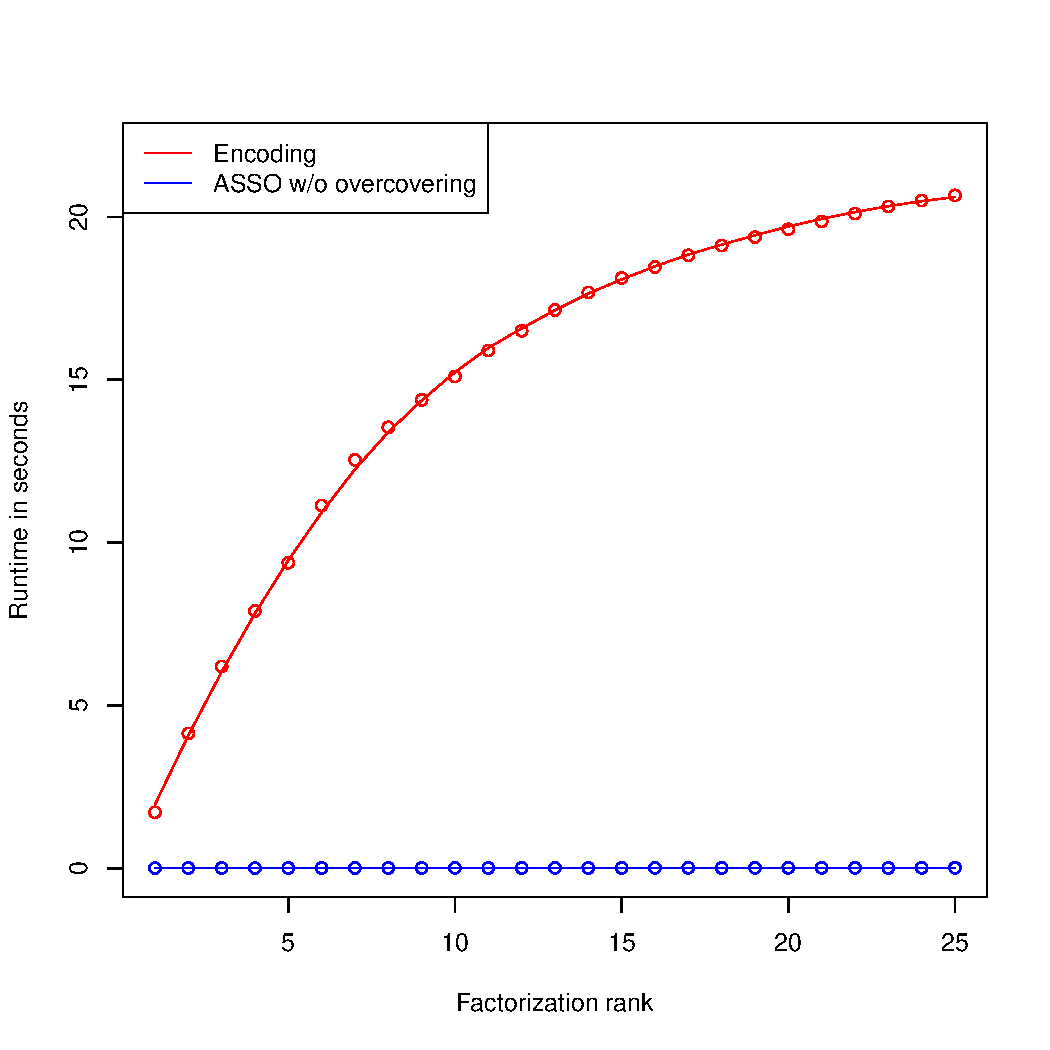
\includegraphics[width=\textwidth]{decomposition_time.pdf}
\caption{Runtime}
\end{subfigure}
   \hfill 
\begin{subfigure}{.49\textwidth}
\centering
\captionsetup{skip=-3pt}
  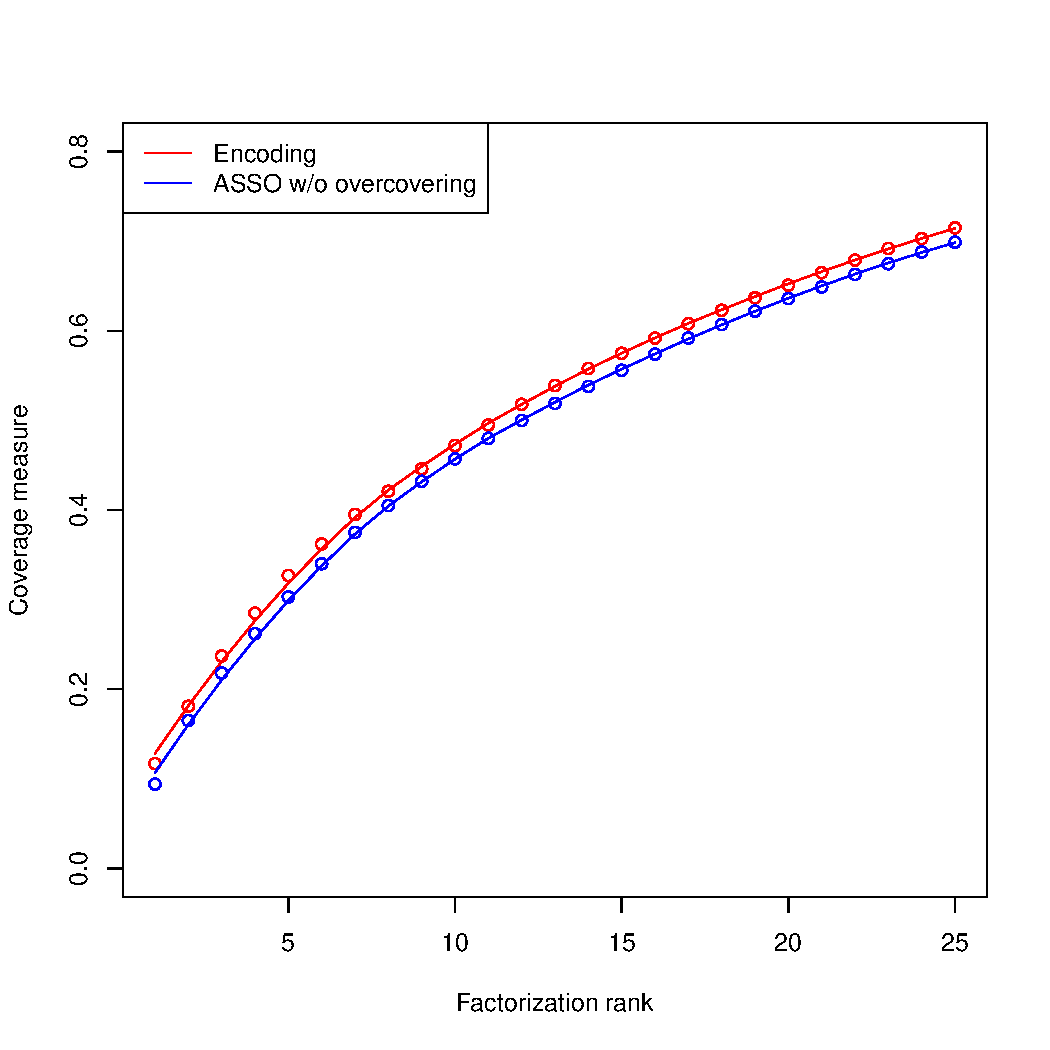
\includegraphics[width=\textwidth]{decomposition_coverage.pdf}
\caption{Coverage}
\end{subfigure}
  \captionsetup{skip=2pt}
  \caption{Boolean matrix factorization on datasets Animals. Runtime and coverage are depicted for different factorization ranks.}
  \label{figure:bmf}
  \end{center}
  \end{figure}

\paragraph{Discriminative pattern set mining}

\begin{figure}[thb]
\begin{subfigure}{.56\textwidth}
  \captionsetup{skip = 0pt}
\begin{center}
  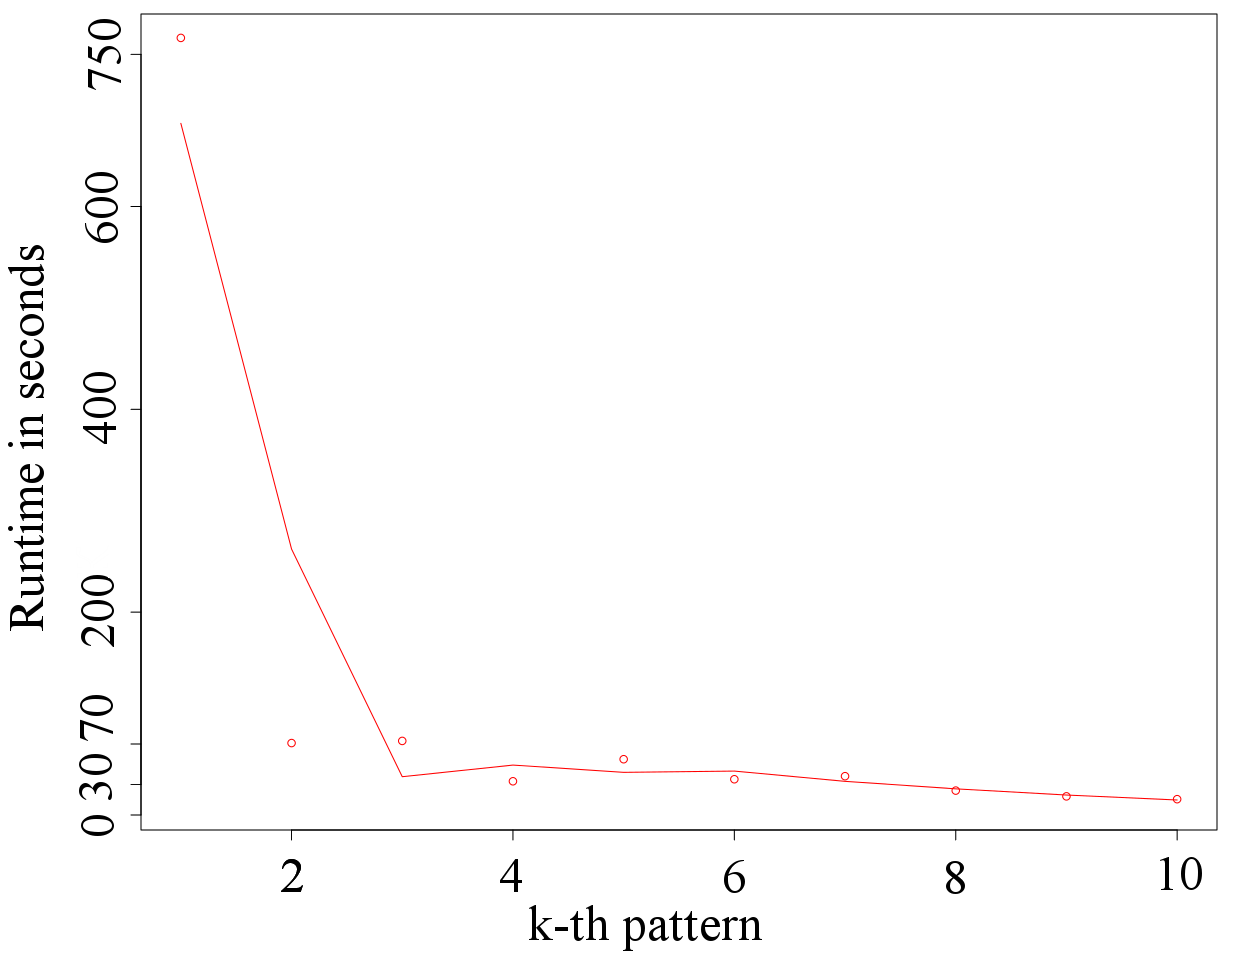
\includegraphics[width=0.9\linewidth]{DiscriminativeChess.png}
  \caption{Runtime (in s) to mine $k$-th discriminative pattern on Chess dataset ($\alpha = 1$, i.e., positive and negative tuples are weighted equally)}
  \label{figure:discriminative_chess}
 \end{center}
\end{subfigure}
\begin{subfigure}{.43\textwidth}
\begin{center}
\captionsetup{skip = 0pt, font=small}
\captionof{figure}{Discriminative mining coverage on Chess and Tic-tac-toe datasets ($\alpha = 1$, i.e., positive and negative tuples are weighted equally)}
\label{table:discriminative_results}
  \scalebox{0.8}{
\begin{tabular}{lll}
  \phantom{Negative }  & Tic-tac-toe ($k$ = 5) & Chess ($k$ = 10) \\ \cline{2-3} \vspace{-8pt}\\
  Covered  $-$              & 92 (27.7\%)           & 160 (7\%)        \\
  Covered  $+$              & 626 (100\%)           & 864 (95.5\%)     \\
  Difference                & 534                   & 704              \\
  Runtime                   & 0.52s                 & 18m48s           
 \end{tabular}
 }
\end{center}
\end{subfigure}
\caption{Discriminative pattern set mining summary: runtime (left) and coverage (right)}
\end{figure}

\begin{figure}[thb]
\begin{center}
\begin{subfigure}{.49\textwidth}
  \captionsetup{skip = -3pt}
  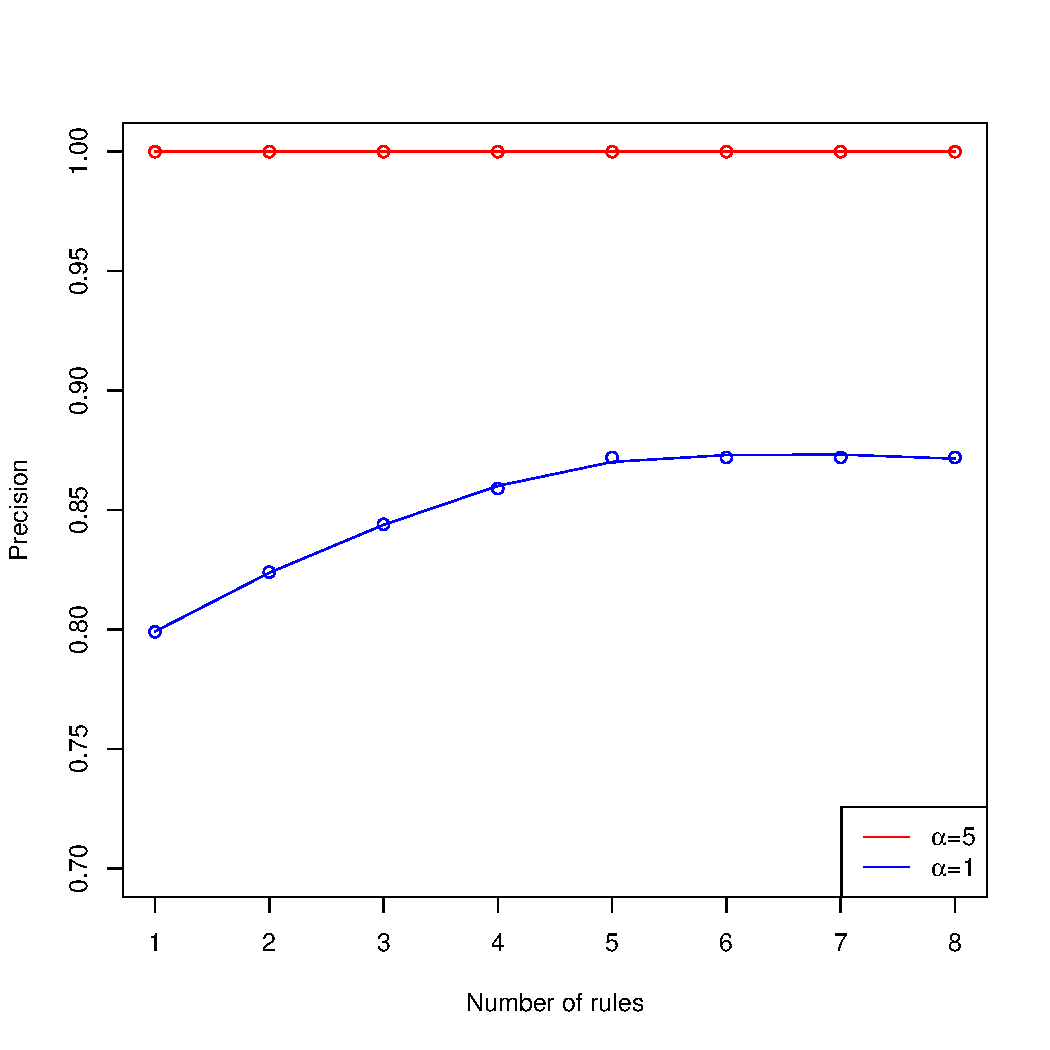
\includegraphics[width=\textwidth]{discriminative_precision.pdf}
  \caption{Precision}
\end{subfigure}
   \hfill 
\begin{subfigure}{.49\textwidth}
  \captionsetup{skip = -3pt}
  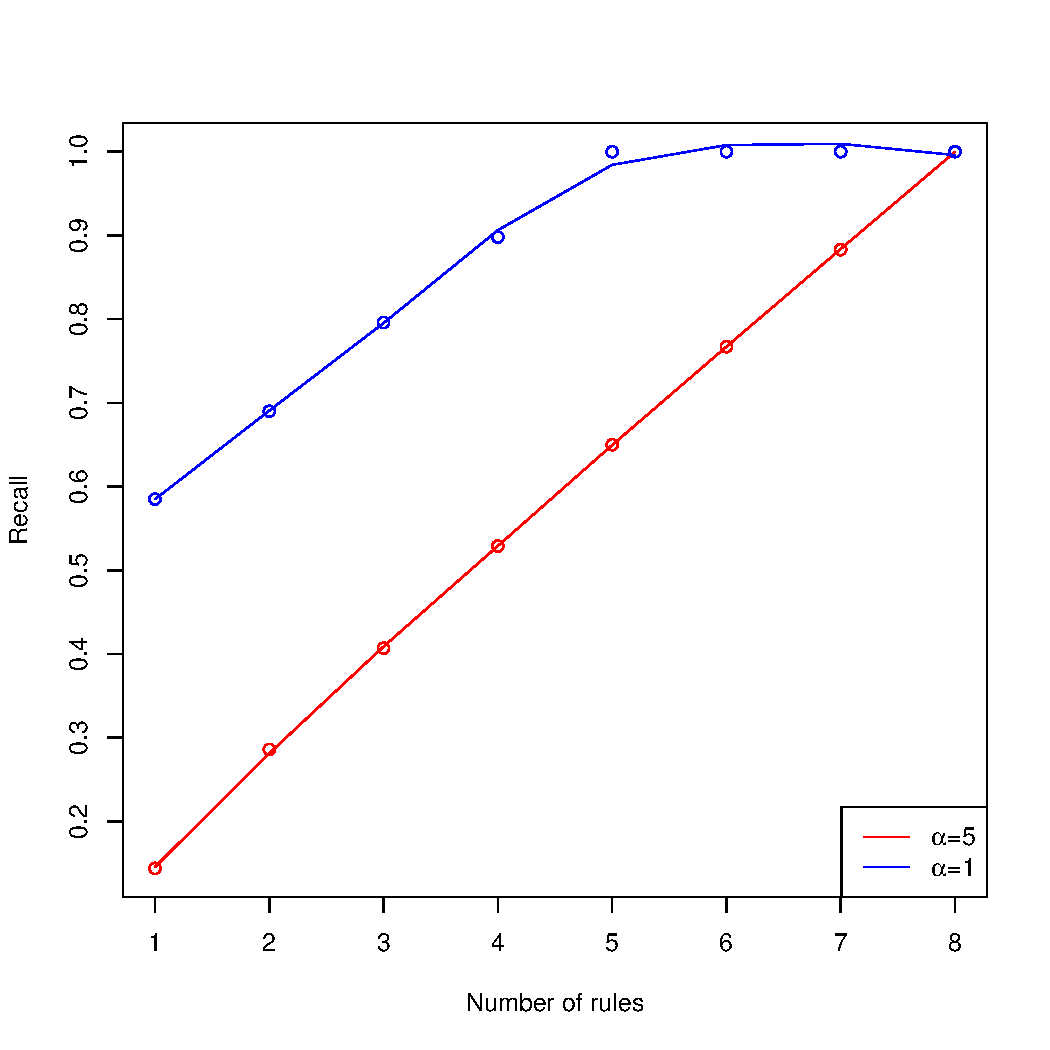
\includegraphics[width=\textwidth]{discriminative_recall.pdf}
  \caption{Recall}
 \end{subfigure}
 \end{center}
  \captionsetup{skip = -4pt}
  \caption{Discriminative pattern set mining (Tic-tac-toe dataset): precision (left) and recall (right) for different $\alpha$, i.e., for varying weights of covering  negative transactions}
  \label{fig:discriminative_precision_recall}
\end{figure}
 Here we demonstrate how the discriminative $k$-pattern mining model from Section \ref{subsec:discriminative} can be solved. For this we use Chess and Tic-tac-toe from Table \ref{table:dataset_description}, each of which has a binary class label indicating whether a game was won or not and can therefore be naturally used for this task. 

We apply the encoding from Listing~\ref{encoding_discriminate} to both datasets, set $\alpha = 1$ to weigh positive and negative tuples equally, and summarize the results in Figure~\ref{table:discriminative_results}. The results show that five patterns suffice to cover all positive examples of Tic-tac-toe, hence mining more than five patterns would be useless. 92 of the 718 covered tuples are negative, i.e., $12.8\%$, while $34.7\%$ of the tuples in the complete dataset is negative. For Tic-tac-toe, the time needed to solve this task is very limited: about half a second.

Figure~\ref{figure:discriminative_chess} shows the runtime needed to iteratively find subsequent patterns in the Chess dataset. Interestingly, it seems that the problem becomes substantially easier (computationally) once the first few patterns have been found: the runtime per pattern drops heavily. This confirms that the search space shrinks when the problem becomes more constrained, i.e., the number of answer sets decreases with the addition of more constraints.

We next show the influence of the $\alpha$ parameter, i.e., the relative weight of covering positive and negative tuples in the optimization criterion. By increasing $\alpha$, the `penalty' for covering a negative tuple is increased and the algorithm can be forced to select more conservative rules. We investigate the effect of this parameter by measuring and comparing precision and recall of the obtained pattern sets for $\alpha = 1$ and $\alpha = 5$. Figure~\ref{fig:discriminative_precision_recall} shows that precision goes to $1$ when $\alpha$ is increased, while recall is decreased but this can be compensated by mining a larger number of patterns\footnote{\changesb Appendix \ref{appendix:precision_recall} presents the data points of Figure \ref{fig:discriminative_precision_recall} as a traditional precision-recall plot.\changese}.

This task differs from the previous one in its optimization criterion: positive coverage penalized by negative coverage allows for fast inference and discovery of the optimal solution, which results in shorter runtimes than for tiling. 

\paragraph{Matrix block-diagonal form}

We apply three versions of the encoding to the Animals dataset \parencite{animalDataset}. The results presented in Figure~\ref{fig:diag_examples} demonstrate that the Animals dataset can be re-arranged into block-diagonal form using our proposed framework. The runtime in all experiments are on the order of seconds. Parameters used in the experiments were $\alpha=\frac{3}{20}$ and $\beta=\frac{1}{20}$. Figure \ref{fig:noisy_block_diagonal} demonstrates the model from Section \ref{subsec:blockdiagonal}, with the same $\alpha$, $\beta$ and $N=1$. The low-level encoding of this model is given in Listing \ref{lst:diag_encoding}.

\subsection{Purely relational data factorization}
\label{subsec:solvingrelational}

\begin{figure}[tbh]
  \centering
  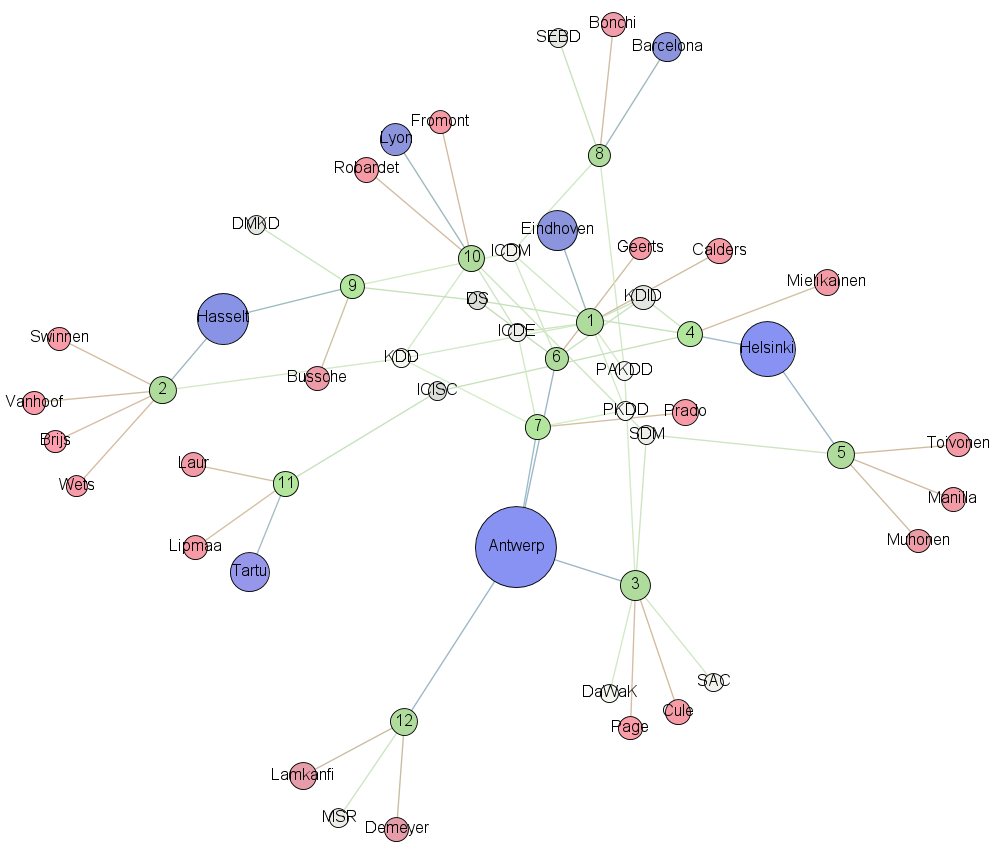
\includegraphics[width=1.00\linewidth]{Bart_clustering.png}
  \captionsetup{skip=-0pt}
  \caption{Clustering in topics by ReDF. Red nodes represent co-authors, blue their university cities, white nodes venues and green topics that bind them  together. If there is an edge between a topic and a node, then there is a corresponding element in the relation (i.e., \textit{interestedIn}, \textit{specializedIn} or \textit{inField}) }
  \label{figure:purely_relational_decomposition}
\end{figure}

In Section~\ref{sec:pure_decomposition} we described how to model the factorization of \textit{publishedIn(Author, University, Venue)} into three binary relations with a latent variable \textit{Topic}. We now evaluate whether the standard ASP solver can solve this task. Unfortunately, we cannot expect a generic solver to handle enormous datasets such as the one from ArXiv as described by \cite{Gopalan2013Efficient}. Instead, we demonstrate a proof-of-concept of solving the model in Listing~\ref{lst:pure_relational_encoding} on a moderate dataset.

We constructed a dataset for a well-known colleague from the data mining community: Bart Goethals (Antwerp University). We collected his publication list from Microsoft Academic Search\footnote{\scriptsize{\url{http://academic.research.microsoft.com/Author/2266478/bart-goethals}}} and extracted for each paper the publication venue, and all co-authors together with their corresponding affiliations (i.e., the last known affiliation for each author in this list of papers). Each unique combination of venue, co-author, and affiliation resulted in a tuple in the \textit{publishedIn} relation. The complete dataset contains 57 tuples over 19 universities, 38 authors, and 15 venues.

Intuitively, if a set of \emph{authors} from a set of \emph{universities} publish in a set of \emph{venues}, then there must be an underlying research \emph{topic} that unites them. Hence, by factorizing the relation into three separate relations, we cluster each of the entity types into a (fixed) number of topics, as indicated by the value of the latent \textit{Topic} variable.

The results for factorization using $K = 12$ topics and $\alpha=\frac{1}{2}$ are presented in Figure~\ref{figure:purely_relational_decomposition}, including co-authors (red), universities (blue), publication venues (purple), and topics (green). To determine the number of topics $K$, we tracked the optimization criterion while increasing $K$ and stopped when this no longer improved.

Since the task is of an exploratory character, we can only qualitatively evaluate the results. We observe that all data mining venues are located together in the center, connected to the same topics. SEBD, an Italian database conference, stands apart, and there is also a separate block for database and computing venues DaWaK and SAC. \changesb Manual inspection of the results indicates the topics (or clusters) to be coherent and meaningful: they represent different affiliations and groups of co-authors that Bart Goethals has collaborated with. For example, topic $5$ contains the SDM conference, the University of Helsinki, and three co-authors specialized in Data Mining. Hence, this topic could be described as ``Data mining collaboration with the University of Helsinki'', which makes perfect sense as Bart Goethals was previously a researcher in Helsinki. \changese

Not all authors are represented in the factorization. How much of the \textit{publishedIn} dataset is covered depends on the number of topics $K$ (which was chosen as described before). The higher the cardinality of the pattern set, the larger the total coverage. The \covered elements positively contribute to coverage, whereas the \overcovered elements contribute negatively. This implies that each pattern is chosen such that the number of \covered and \overcovered elements are balanced and the optimization criterion is maximized. In general, covering all authors with few patterns would lead to significant overcovering of the original dataset, while introducing too many patterns would create clusters with only one author (which is clearly undesirable, since these clusters would not be meaningful). 

\changesb The decompositions, as the one depicted in Figure \ref{figure:purely_relational_decomposition}, could serve as a basis for new analyses. For example, we might visualize the intersection of common (latent) topics shared by two researchers. We outline possible examples in Appendix \ref{appendix:application_purel_relational}. \changese


\paragraph{Relational factorization without a latent variable.} In Section \ref{sec:pure_decomposition}, we also described a factorization that does not use any latent variables (analog to the \emph{sells} example in Listing \ref{lst:sells} from the introduction section). We evaluate this model using Listing \ref{lst:pure_alternative} on the same dataset as used in the previous experiment, i.e., the co-author relation \textit{publishedIn(Author, Uni, Venue)} for Bart Goethals.

In general, factorizations do not perfectly match the original relation (i.e., $\error \neq 0$), but in this particular case the system found a lossless solution. It is easy to see that this will not always be possible though. For instance, let us assume we keep multiple affiliations per author in the dataset. For example, apart from a fact $\textit{p(bonchi,barcelona,pakdd)}$, there may be another fact $\textit{p(bonchi, pisa, pakdd)}$ in \textit{publishedIn}. Although the same factorization would be found by the solver, the found solution would be imperfect as the latter fact is not represented in the factorized relation.

Solving this task was computationally easy, since there is no latent variable to iterate over: the runtime was only $0.01s$. Table \ref{table:pure} presents a summary.
\begin{table}[tbh]
\begin{center}
\caption{Experimental summary for pure relational factorizations from Subsection \ref{subsection:beoynd}}
\label{table:pure}
\scalebox{.75}{
\begin{tabular}{llllll}
  \multirow{2}{*}{\textbf{\normalsize{With a latent variable}}} & \textbf{\#Transactions} & \textbf{Overall runtime} & \textbf{Avg runtime} &  \textbf{\#Topics}  &  \textbf{Avg atoms per topic}\\
   & 58  & 14s & 1.1s & 12 & 5.4\\
  \multirow{2}{*}{\textbf{\normalsize{Without a latent variable}}} & \textbf{\#Transactions} & \textbf{Overall runtime} & \textbf{Correct} &  \textbf{\#Incorrect}  &  \textbf{Avg factor size}\\
  & 58  & 0.01s & 58 & 0 & 45
\end{tabular}
}
\end{center}
\end{table}

\paragraph{Relational discriminative learning}
Here we investigate discriminative learning in the purely relational setting, for which we use the discriminative optimization criteria described in Section \ref{sec:pure_decomposition}. For this experiment we collected DBLP data for two well-known researchers in the field of data mining: Jiawei Han and Philip S. Yu. In this example all publications belonging to either researcher are considered a class. Since DBLP data does not have authors affiliations, we replace this attribute with the publication date converted to a categorical variable $M \in \{ \textit{old}, \textit{recent}, \textit{new} \}$, using the following rule: if the date is later than 2010, it is represented as ``new''; if it is between 2005 and 2010, then it is ``recent''; otherwise it is ``old''. The complete dataset contains around 6000 ground atoms of the following form: \textit{paper(Author,Age,Venue,Han$\backslash$Yu)}. The goal is to predict whether the paper is co-authored by Han or Yu based on author, venue and age using discriminative rules as defined in Eq. \ref{eq:pure_relational_discriminative}. In this experiment the shape is
\begin{equation*}
  \appr(A,M,V) \leftarrow \textit{author}(A,T), \textit{paperAge}(M,T), \textit{venue}(V,M),
\end{equation*}
where $T$ is a latent variable. As for the previous discriminative experiment, in Figure \ref{fig:discriminative_precision_recall_relational} we present an overview of the dependency of precision and recall on the number of patterns and $\alpha$, the penalty for covering the incorrect class. Runtimes are similar as in Figure \ref{figure:discriminative_chess}. ASP finds an optimal solution in half an hour and then spends a substantial amount of time to prove it is indeed the best solution. We therefore used a time limit of one hour per pattern speedup the computation. This limit was only reached in the computation of the first pattern, for both values of $\alpha$.

In Figure \ref{fig:discriminative_precision_recall_relational} we see that, depending on the number of patterns and penalty for covering the wrong class ($\alpha$), we can obtain a classifier with different precision and recall%The specific choice for the number of patterns and penalty is typically domain-specific and is therefore beyond the scope of this paper.
\footnote{\changesb Appendix \ref{appendix:precision_recall} presents the data points of Figure \ref{fig:discriminative_precision_recall_relational} as a traditional precision-recall plot.\changese}.


\begin{figure}[thb]
\begin{center}
\begin{subfigure}{.49\textwidth}
  \captionsetup{skip = 2pt}
  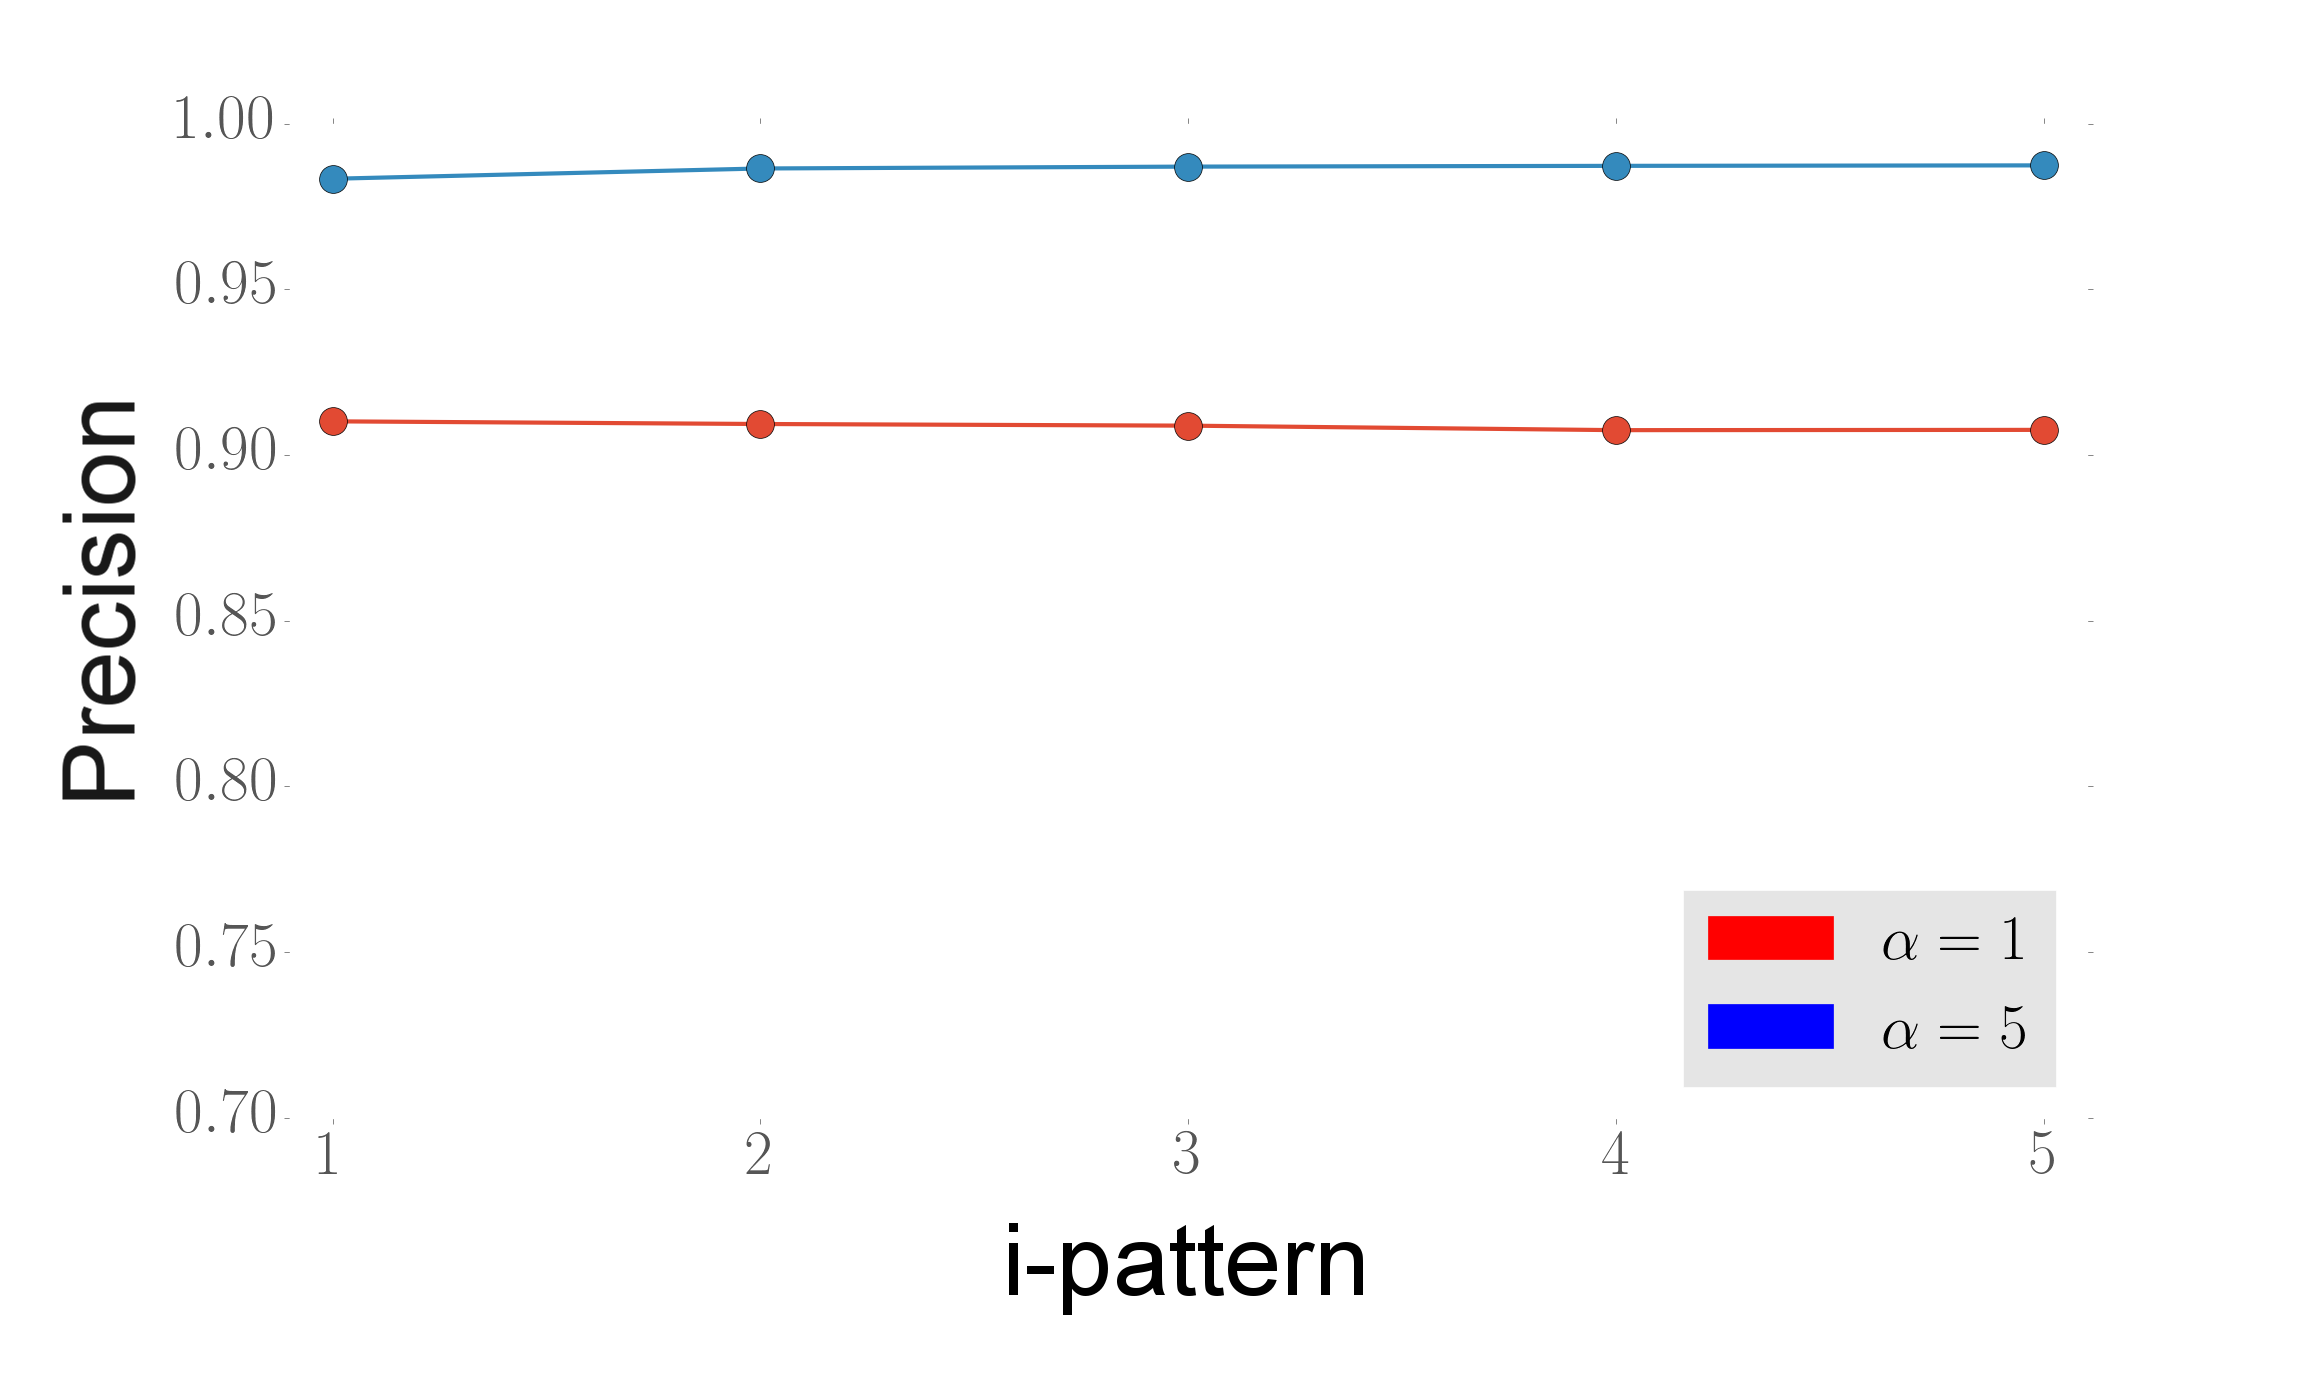
\includegraphics[width=\textwidth]{discriminative_precision_relational.png}
  \caption{Precision}
\end{subfigure}
   \hfill 
\begin{subfigure}{.49\textwidth}
  \captionsetup{skip = 2pt}
  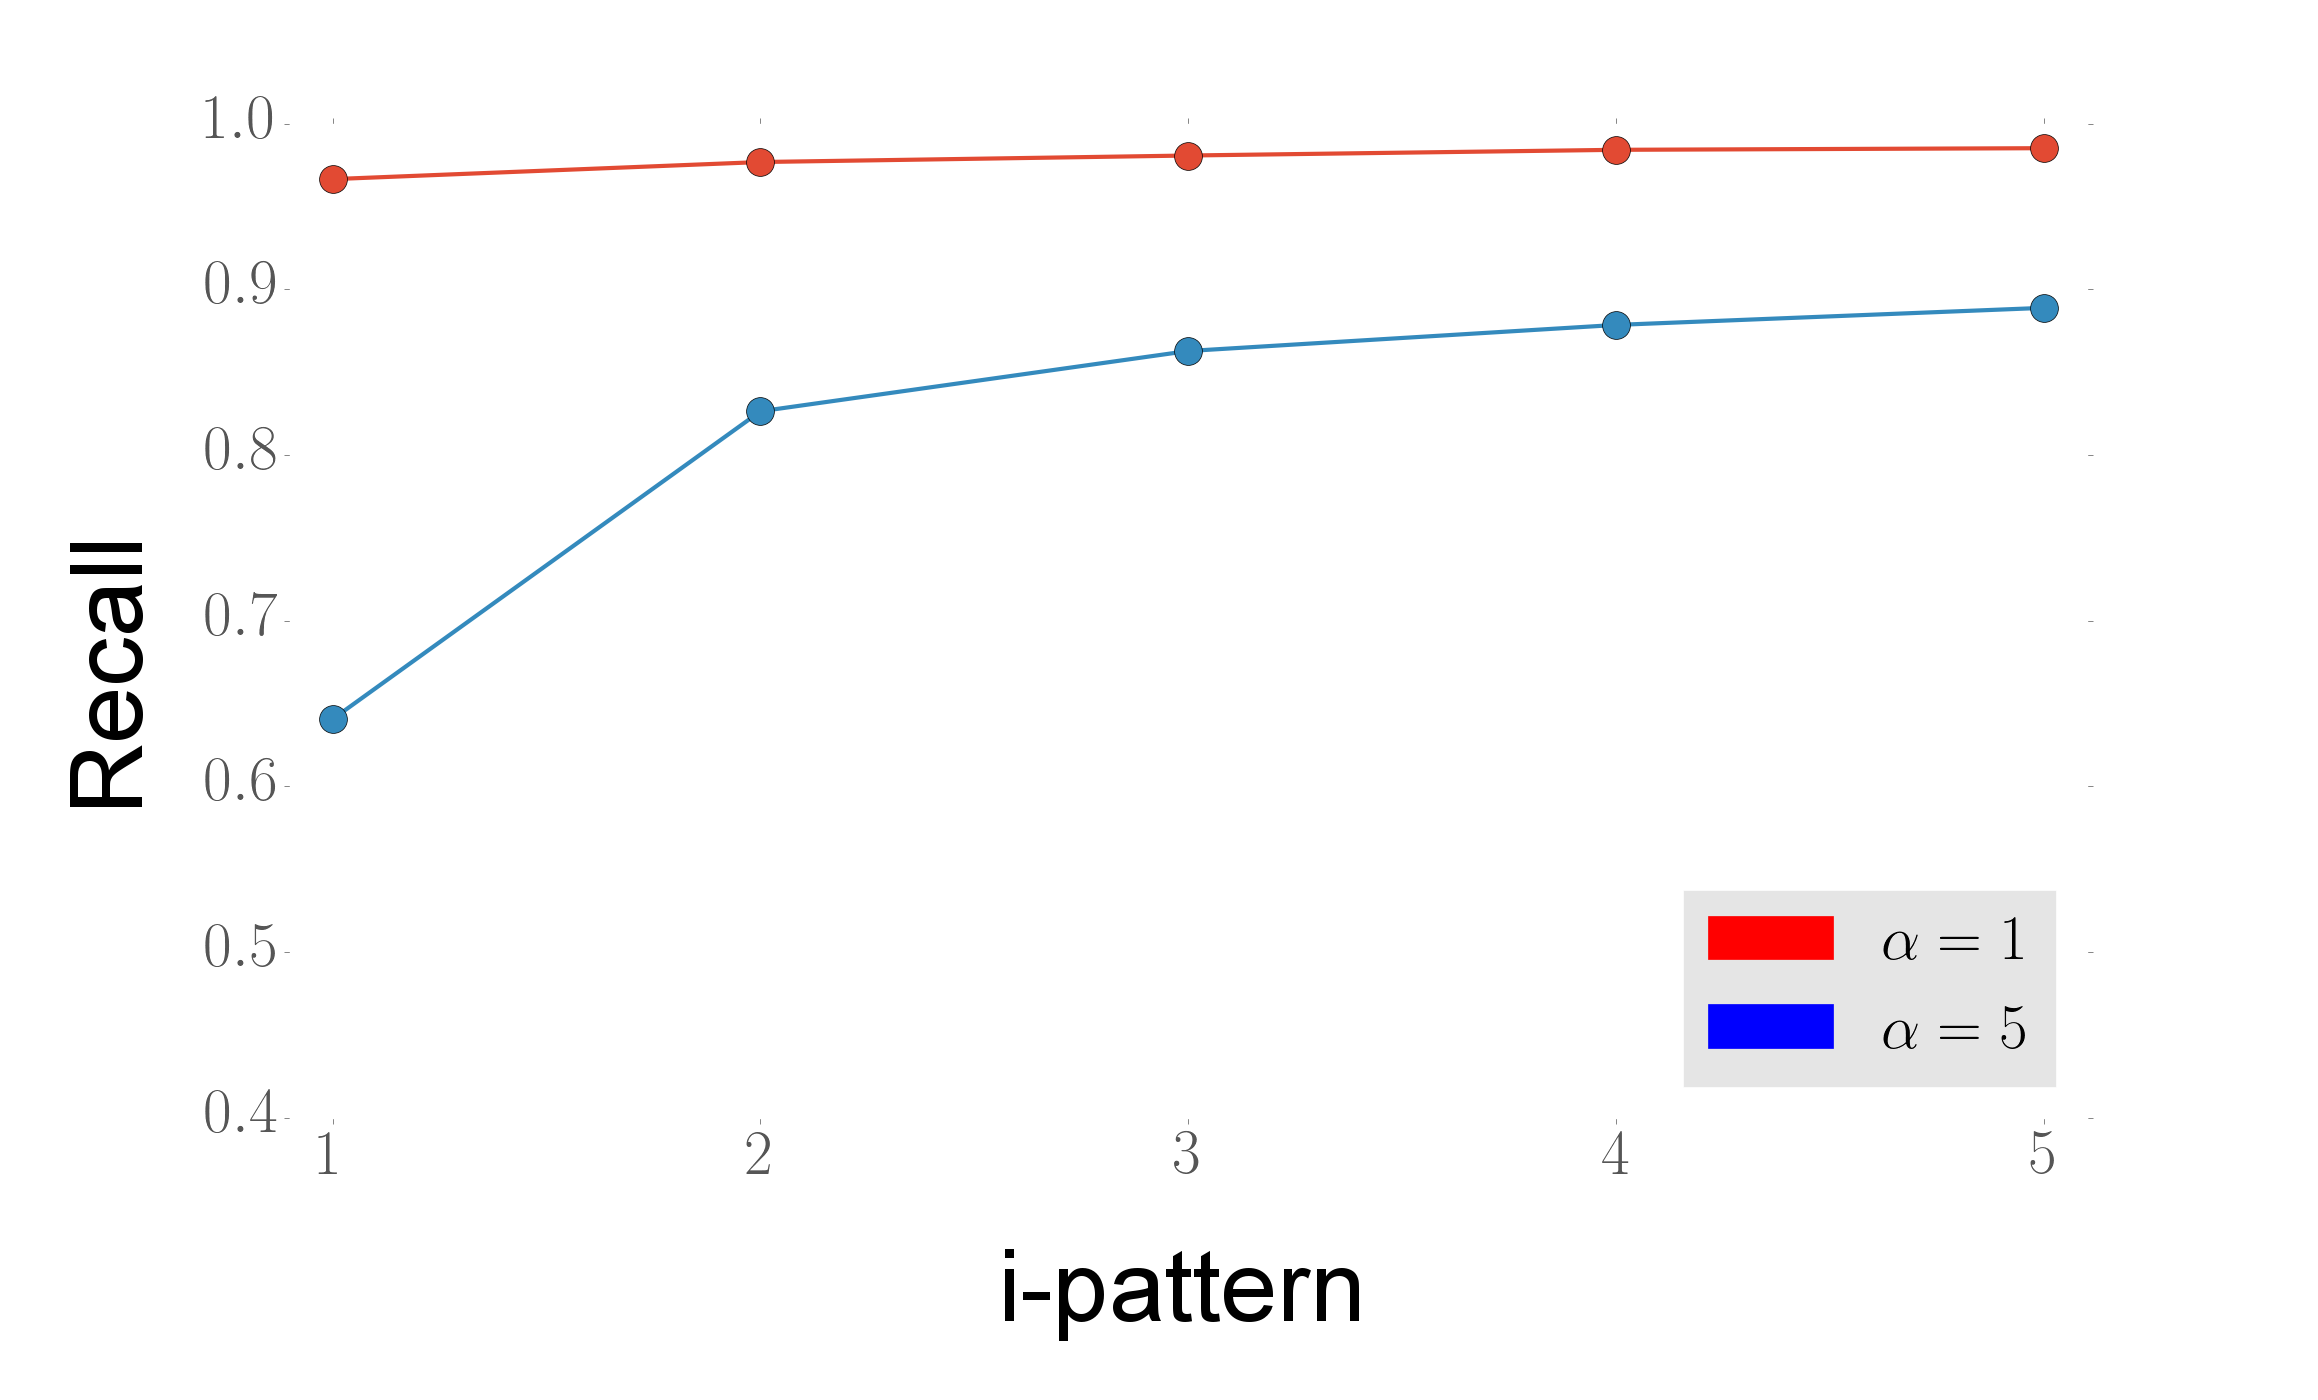
\includegraphics[width=\textwidth]{discriminative_recall_relational.png}
  \caption{Recall}
 \end{subfigure}
 \end{center}
  \captionsetup{skip = -4pt}
  \caption{Discriminative learning in the purely relational setting; precision (left) and recall (right) for different $\alpha$, i.e., for two weights of covering negative atoms.}
  \label{fig:discriminative_precision_recall_relational}
\end{figure}
\subsection{Runtime discussion} 

In this section we have seen a number of experiments that solve ReDF problems using generic solving technology, i.e., answer set programming. As we can see in Figures \ref{fig:tiling_time_comparison} and \ref{figure:bmf}, specialized algorithms are substantially faster than ASP. On datasets of moderate size, however, generic solvers obtain reasonable runtimes, as indicated by the results in Tables \ref{tab:tiling:time}, \ref{tab:overlapping:time}, and \ref{table:discriminative_results}, and Figures \ref{figure:bmf} and \ref{figure:discriminative_chess}. For the purely relational data factorization task from Section \ref{sec:pure_decomposition} we present a summary of the experiments in Table \ref{table:pure}. In these experiments, computation time ranged from several seconds to few minutes.

%Figure \ref{fig:regular_block_diagonal} demonstrates the simplified model from Section \ref{subsec:blockdiagonal}, where instead of constraint \overcoverageConstraint we use \noiseConstraint and we omit the second part (indicated by Eq. \ref{trans_penalty} and \ref{item_penalty}) of optimization function \ref{eq:block_diagonal_optimization}. It does not introduce any penalties for unmatched elements in the same rows and columns as the tile uses, and it does not tolerate presence of the noise in tiles. Figure \ref{fig:penalty_block_diagonal} demonstrates the simplified model from the same section but with penalties, i.e., with the full optimization function. 




\section{Evaluating solver performance}  \label{subsec:evaluatingsolver}
\begin{figure}[htb]
\begin{center}
\begin{subfigure}{.47\textwidth}
    \captionsetup{
     skip=-12pt
     }
  \caption{Runtime (in s) for individual tiles}
  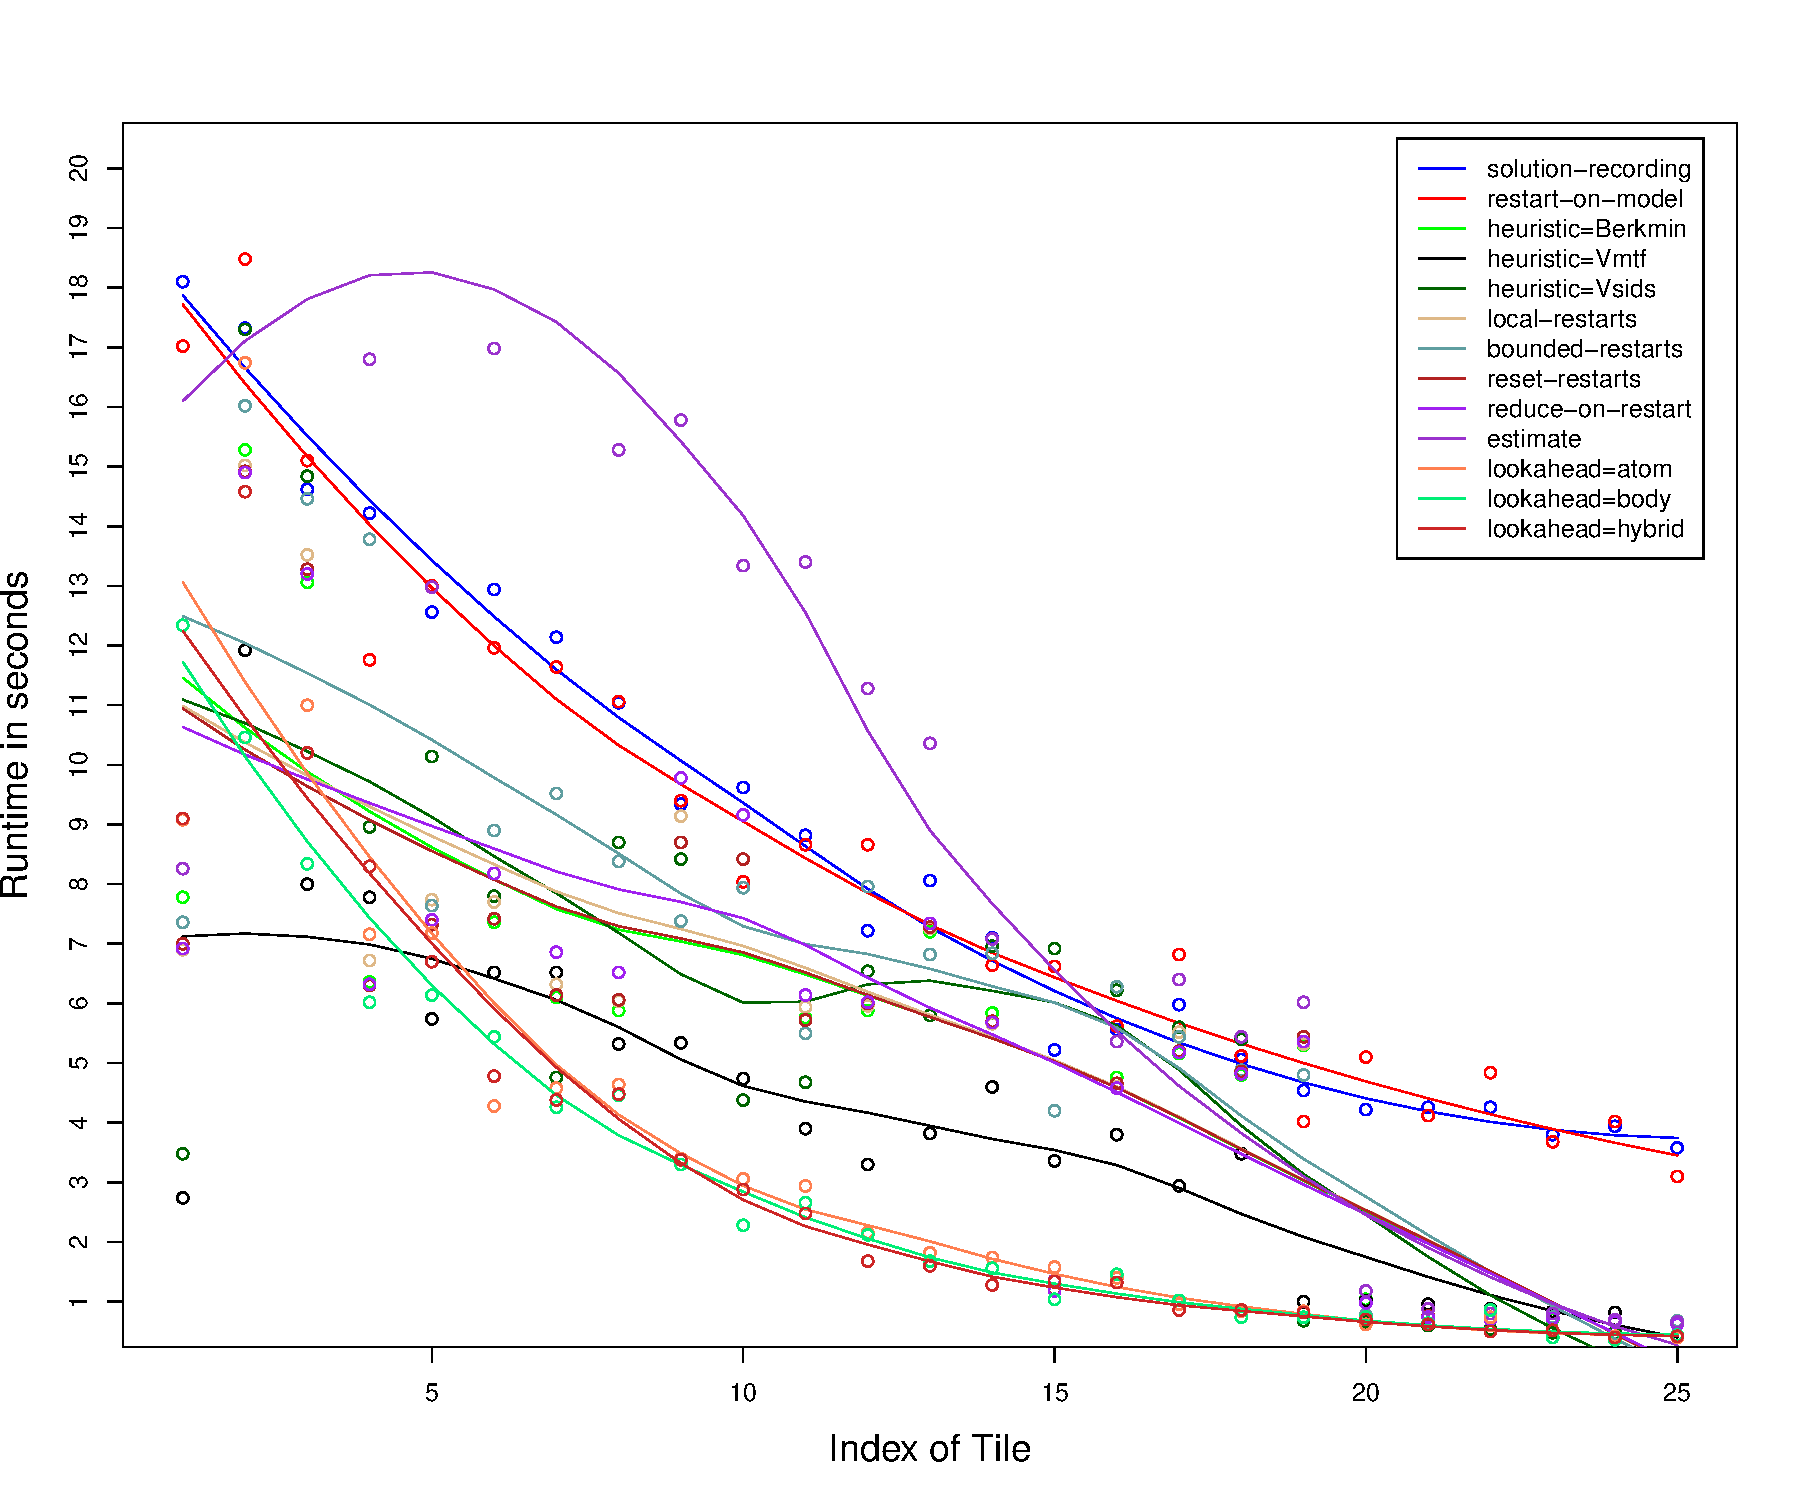
\includegraphics[width=1.12\textwidth]{time_parameters.pdf}
\end{subfigure}
   \hfill 
\begin{subfigure}{.47\textwidth}
  \caption{Runtime (in s) for $N$ tiles}
   \scalebox{.75}{
  \begin{tabular}{lrrrrr}
    \phantom{Search option} & \multicolumn{5}{c}{\textbf{Number of tiles}}\\
     \textbf{Search option} &  \textbf{5}     & \textbf{10}      &  \textbf{15}     &   \textbf{20}   &  \textbf{25}    \\
   \hline
  solution-recording  & 76  &131   & 168  & 193 &  213\\
  restart-on-model    & 75  &127   & 164  & 191 &  211\\
  heuristic=Berkmin   & 50  &86    & 112  & 133 &  137\\
  \textbf{heuristic=Vmtf}      & \textbf{36}  &\textbf{64}    & \textbf{83}   & \textbf{95}  &  \textbf{100}\\
  heuristic=Vsids     & 54  &88    & 119  & 138 &  140\\
  local-restarts      & 49  &87    & 113  & 134 &  138\\
  bounded-restarts    & 59  &101   & 132  & 154 &  158\\
  reset-restarts      & 48  &85    & 111  & 132 &  136\\
  reduce-on-restart   & 48  &89    & 115  & 136 &  139\\
  estimate            & 86  &169   & 213  & 237 &  241\\
  \textbf{lookahead=atom}    & \textbf{51} &\textbf{71}   & \textbf{81}  & \textbf{86} &  \textbf{88}\\
  \textbf{lookahead=body}    & \textbf{43} &\textbf{63}   & \textbf{72}  & \textbf{76} &  \textbf{79}\\
  \textbf{lookahead=hybrid}  & \textbf{48} &\textbf{68}   & \textbf{77}  & \textbf{81} &  \textbf{84}\\
   \end{tabular}
}
\phantom{teeext}\\
\end{subfigure}
  \caption{Determining the best ASP solver parameters for tiling with the model of Listing~\ref{lst:encoding}: (a) the runtime (in s) needed for mining each subsequent individual tile, (b) runtime summary (in s) for first 25 tiles}
  \label{meta-time}
\end{center}
\end{figure}

This appendix briefly evaluates the performance of the solver that was used for the experiments. We first describe how we tuned the system and then continue with an analysis of the solving process.

\textit{Solver tuning.} The clingo system \parencite{gebser2011potassco} has a variety of parameters that affect runtime. We performed a series of preliminary experiments to determine the parameters that were used for all other experiments in this section. These tuning experiments mostly concerned maximum $k$-tiling on datasets of moderate size, but some test experiments on other tasks did not reveal any discrepancies. 

Runtime was measured for a large number of search options while fixing the dataset and task. Figure~\ref{meta-time} shows the results obtained for maximum $k$-tiling on the Animals dataset. 
Search options ``heuristic=Vmtf'' and the ``lookahead'' options result in shorter runtimes, but the ``lookahead'' options do not scale well; with these options the system is unable to handle bigger datasets like Mushroom and Chess. Therefore, all remaining experiments in this section have been performed with ``heuristics=Vmtf''. None of the other combinations of parameters gave any substantial improvement in runtime.

\textit{Grounding-solving analysis} Besides measuring the time needed for the solver to provide an answer, it is also useful to look at the time needed for the individual execution steps. In case of answer set programming, solving a problem consists of two main steps: 1) grounding and 2) solving (or, alternatively, searching). 

Table~\ref{table:steps-time} presents results obtained for the maximum k-tiling problem, i.e., the time needed to compute a single tile, averaged over the first 15 tiles, split into grounding and solving time. For many ASP programs the grounding step is the bottleneck, but the results clearly demonstrate that this is not the case for our ReDF tasks: the ratio between solving and grounding time is generally large. (Due to long runtimes this experiment was not performed for Chess and Mushroom.)

The large ratios can be explained by the fact that we deal with optimization problems, as is usual in data mining. In the presence of an exponential number of answer sets and a binary predicate as the optimization criterion, it is natural to expect the solving part to be the computationally most intensive step. 

The results suggest that, if we would like to speed-up ReDF in ASP, we would have to focus on making the general solving process more efficient, possibly by using properties of the ReDF framework. Specialized mining algorithms, e.g., for tiling, demonstrate that faster solving is possible, but translating these efficient mechanisms to an ASP solver, which works completely differently, seems far from trivial.

\begin{table}\footnotesize
  \caption{Maximum k-tiling: grounding and solving -- avg time per tile (s), and their time ratio}
  \label{table:steps-time}
\vspace{-10pt}
\begin{center}
\begin{tabular}{lrrc}
  Dataset & Grounding & \phantom{text} Solving & \phantom{aaa} Ratio -- Solving/Grounding \\ \hline
Nursery     &2.173&38.185 & 18 \\
Voting      &0.052&8.350 & 161  \\
Animals     &0.020&2.728 & 136 \\
Tic-tac-toe &0.124&1.969 & 16  \\
Flare       &0.225&0.575 & 3
\end{tabular}
\end{center}
\end{table}

\textit{Alternatives to manual parameter tuning.} \textit{Claspfolio} is a portfolio system for Clasp \parencite{gekakascsczi11a}. However, our experiments indicated that none of the precomputed models of Claspfolio applied to the problems considered in this work and the system switches to the default solver. \textit{hClasp} \parencite{conf/aaai/GebserKROSW13} introduces heuristics into the reasoning process of Clasp. Since we consider a wide class of problems, it requires a nontrivial decision procedure to find the right heuristics for a particular task. We regard it as a possible direction for future research.



\section{Visualizations for an application of purely relational ReDF}\label{appendix:application_purel_relational}
Figures \ref{fig:instersection_purely_relational_floris} and \ref{fig:instersection_purely_relational_pauli} visualize an example application of purely relational factorization. Figure \ref{fig:instersection_purely_relational_floris} shows the intersection of latent topics depicted in Figure \ref{figure:purely_relational_decomposition} with publication data of Floris Geerts, while Figure \ref{fig:instersection_purely_relational_pauli} shows the intersection of the same latent topics with the publication data of Pauli Miettinen. 

The figures show that we can relate not only particular data points such as venues and co-authors between scientists, but also common (latent) topics. They are identified and visualized in an interpretable manner. The intersection includes the publication records (indicated in red) of two authors (the other author is indicated in pink, if he/she belongs to co-authors of the original decomposition). If for a latent variable, there are a co-author, a university and a venue that belong to both authors, then the latent topic is labeled (in blue) as common.
\begin{figure}[htb]
  \begin{center}
      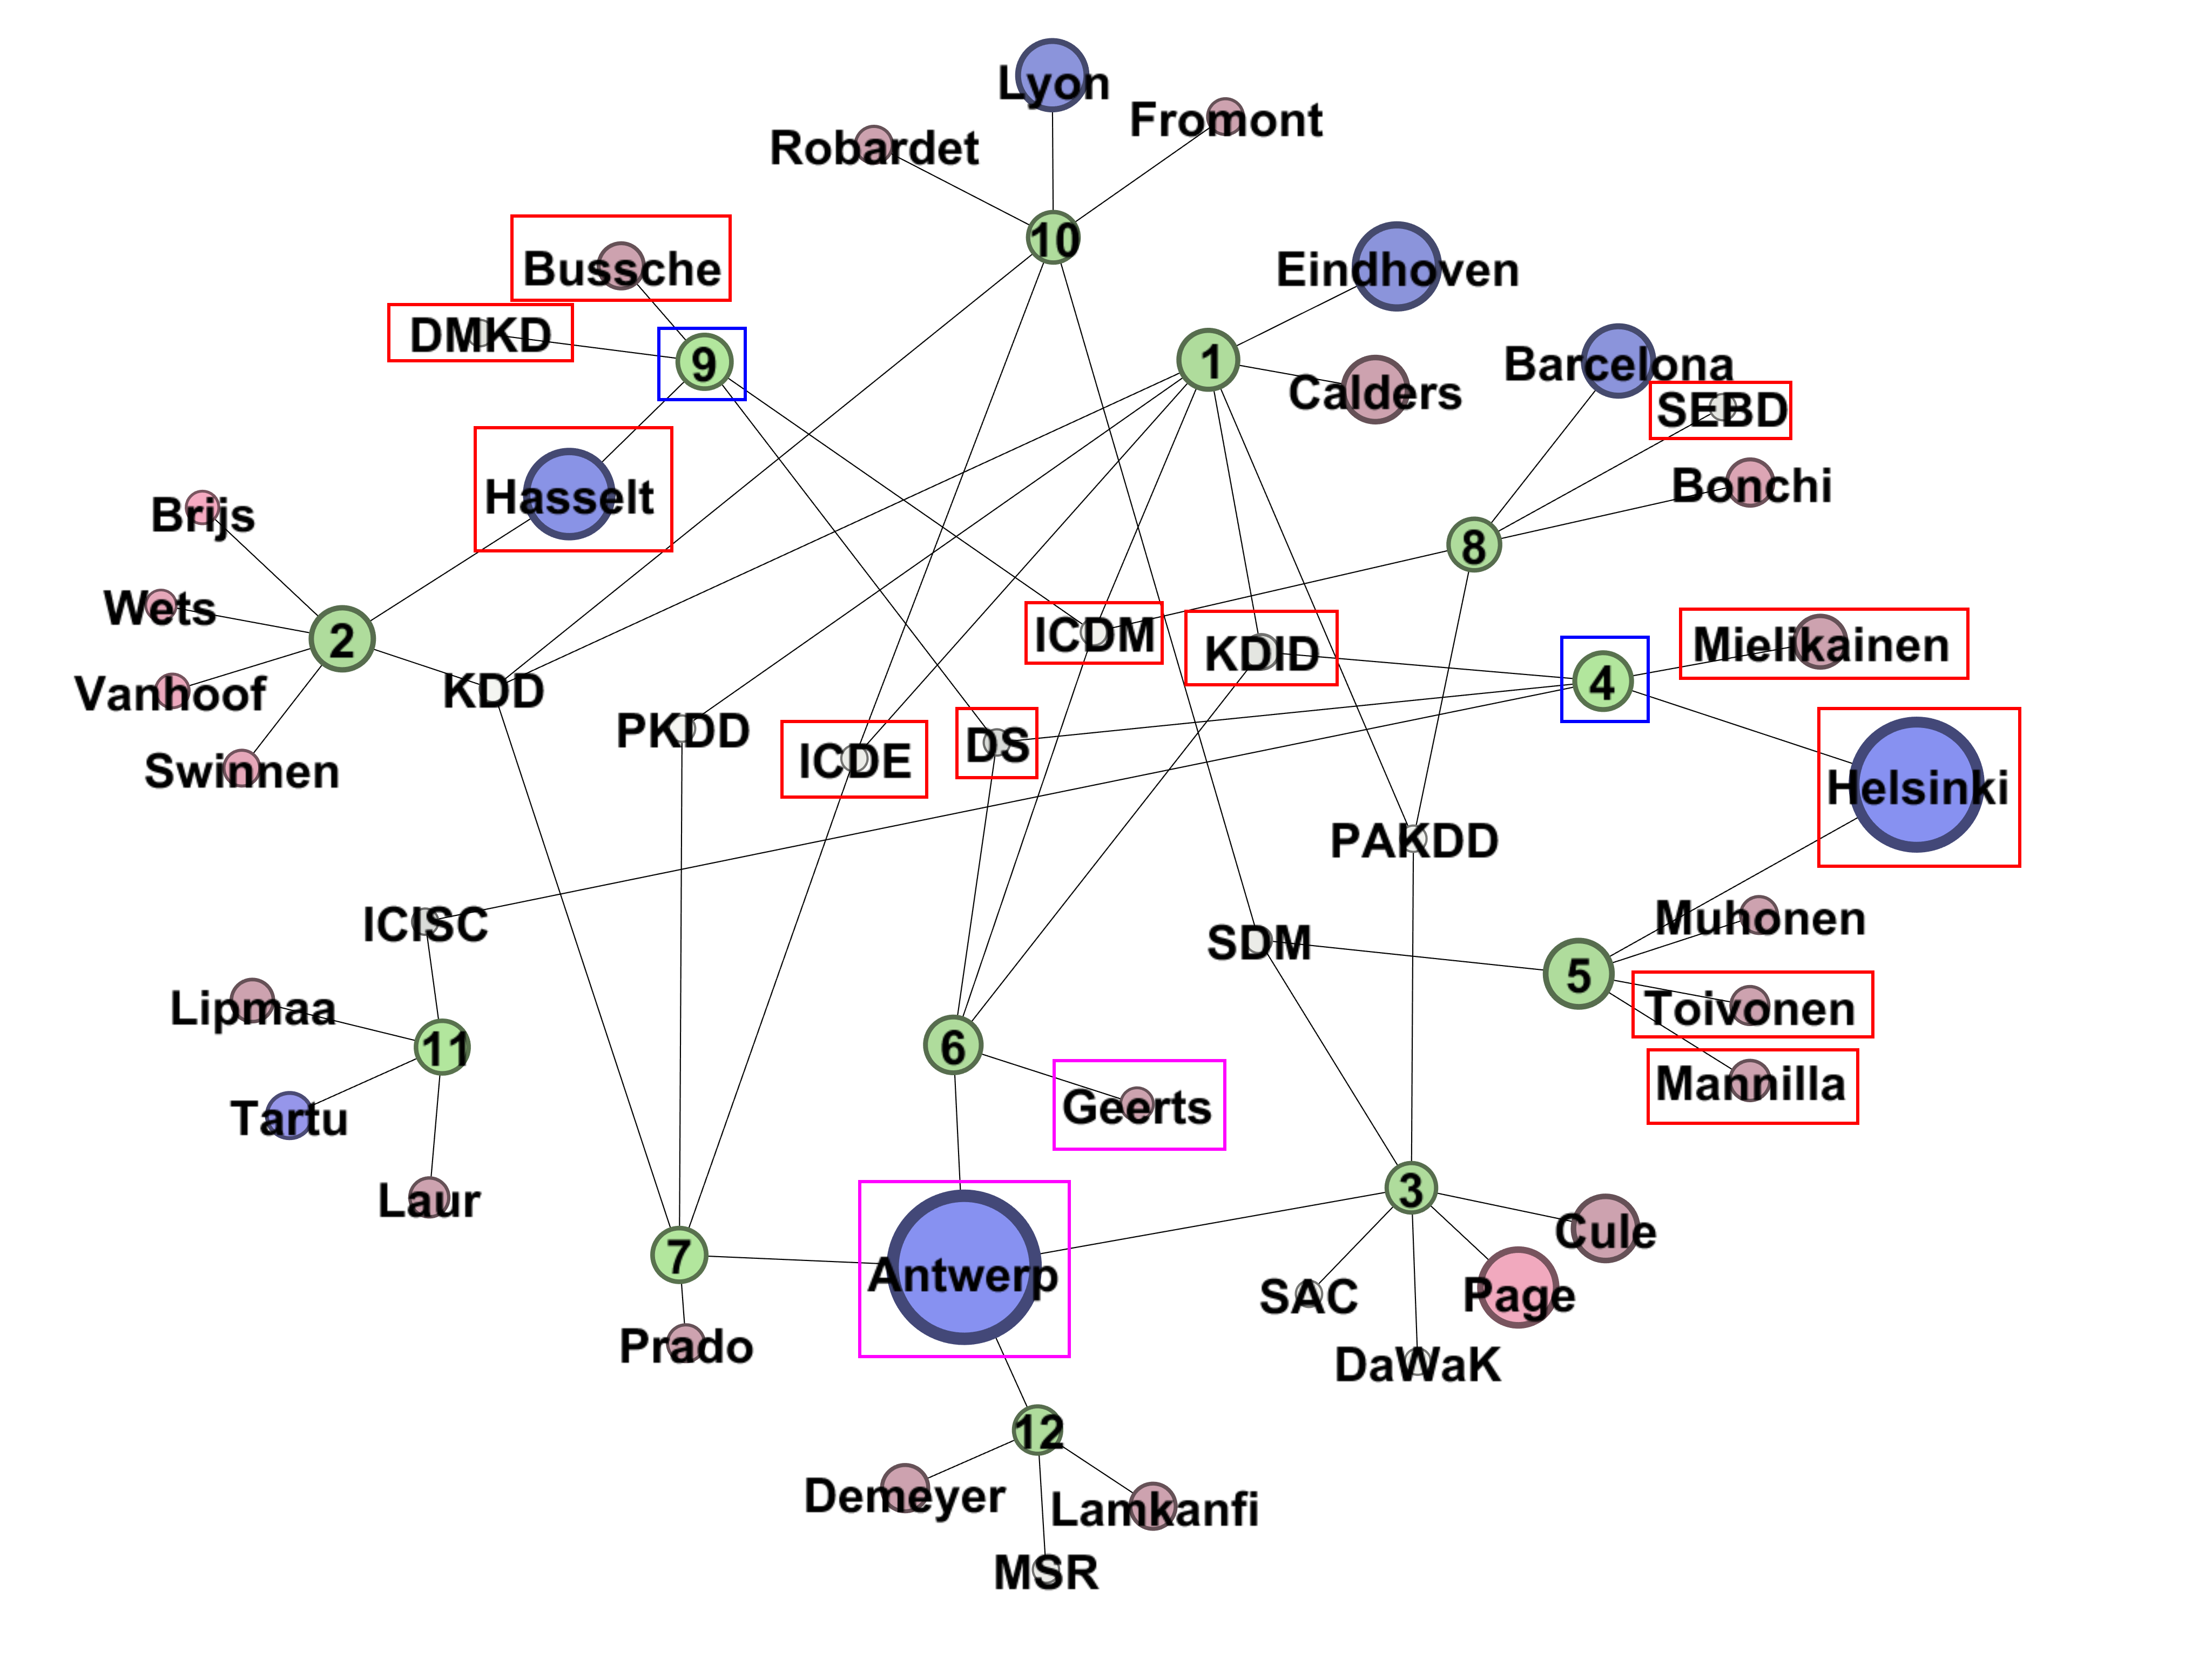
\includegraphics[width=\textwidth]{query_relational_selection_floris_geerts.png}
  \end{center}
  \caption{An application of purely relational factorization: intersection of publication data (in red) and latent topics (in blue) of Bart Goethals with publications of his co-author Floris Geerts (highlighted in pink) in the graph. A latent topic belongs to an intersection if both have the same co-author, university and venue in the publication records.}
  \label{fig:instersection_purely_relational_floris}
\end{figure}

\begin{figure}[htb]
  \begin{center}
      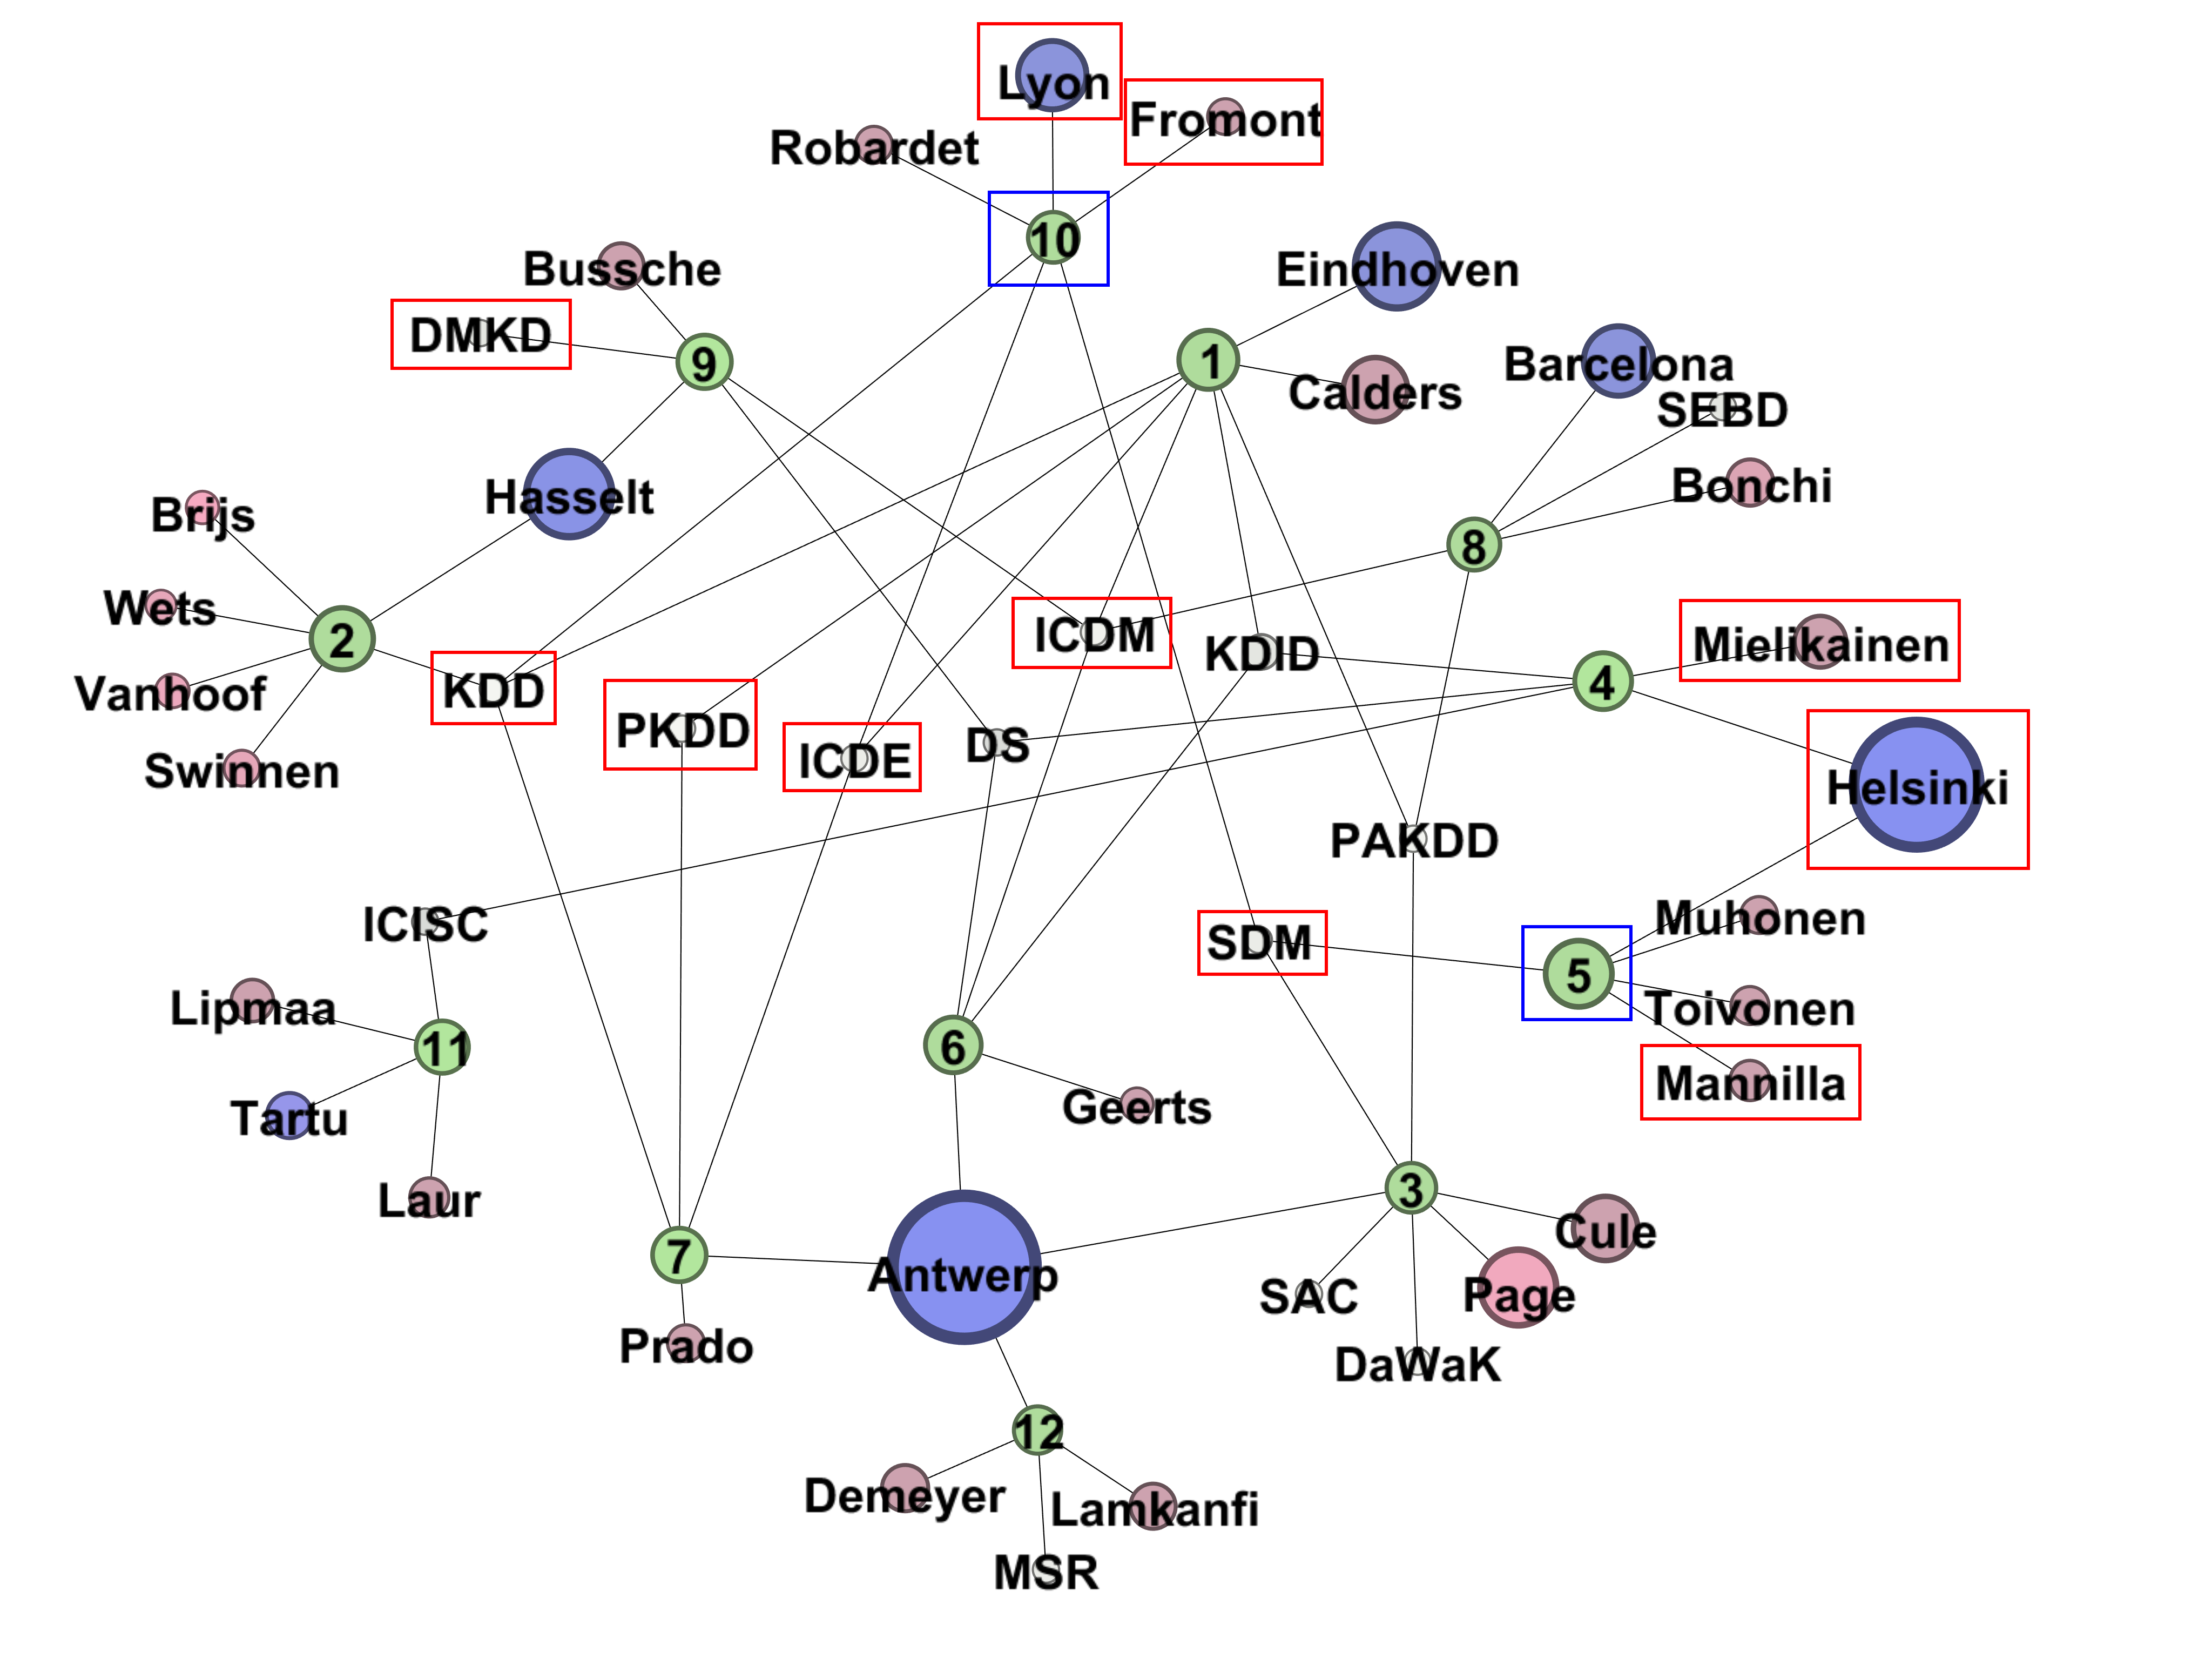
\includegraphics[width=\textwidth]{query_relational_selection_pauli_miettens.png}
  \end{center}
  \caption{An application of purely relational factorization: intersection of publication data (in red) and of latent topics (in blue) of Bart Goethals with publications of Pauli Miettinen (not his co-author). A latent topic belongs to an intersection if both have the same co-author, university and venue in the publication records.}
  \label{fig:instersection_purely_relational_pauli}
\end{figure}



\section{Maximum $k$ set coverage analysis of greedy strategy}\label{appendix:k_set_coverage_analysis}
We here elaborate on the bounds of the greedy and sampling strategies as described in Algorithms \ref{alg:greedy} and \ref{sampling}, when applied to the problems we consider in this work.

In the greedy case of Algorithm \ref{alg:greedy}, the bound analysis is similar to LTM-$k$ and based on the analysis of the greedy approach to general maximum $k$-coverage \citep{max_k_set_cover1, max_k_set_cover2}. Greedy search optimizes its result in each iteration, given the solutions from the previous iterations, until $k$ solutions have been found. Hence, this algorithm follows the general maximum $k$-coverage strategy and the factor $\frac{\textit{greedy}}{\textit{optimal}} \leq 1-\frac{1}{e}$ applies.

The key assumption highlighted by \citet{max_k_set_cover1} is that for a set selected in the $i^{th}$ iteration, no data point can be counted twice, i.e., in two different sets, towards the maximal weight summary. That is, if a data point is present in the sets selected in previous iterations, then the total weight should be the same as if we excluded this data point from one of the sets; the solutions should be non-overlapping. This is the case for the problems we consider (tiling, discriminative rule mining, tiling-based matrix diagonalization, etc).

Furthermore, the maximum $k$-set cover bound is very general and in practice, the greedy solution is way closer to the optimum than suggested by the bound. For example, \citet{GunsNR13} presented a constraint model of optimal tiling and based on this it was possible to compute the optimal $k$-tiling for $k=2$ for the smallest datasets and for $k=3$ for two datasets (a time-out was set to 6 hours). The average difference between optimal and actual area across all datasets was around $1\%$, while the bound suggests that it might deviate up to $36.7\%$.

The sampling strategy of Algorithm \ref{sampling} follows the approximate greedy scheme: on each iteration it greedily finds an approximation of a `greedily optimal' solution. As has been shown by \cite{max_k_set_cover1}, the approximate greedy schema with approximation parameter $\beta$ (i.e., a solution found at $i$-th iteration is within a $\beta$ constant factor of the greedy optimal one at $i$-th iteration) is within $1-\frac{1}{e^\beta}$ from the optimal solution.

$\alpha$, the parameter controlling the number of columns to sample, influences both runtime and coverage, i.e., solution quality. It is, however, extremely hard---if not impossible---to analytically derive the dependency between sample size $\alpha$ and approximation factor $\beta$, given the generality of the method. Many existing methods used to obtain sampling bounds rely on a) (model) distributions, or its forms, on the parameters and/or values (observed and/or latent) in the data, b) the structure of the constraints, c) the form of the optimization function. In our case, we consider a very generic sampling method and therefore determining an exact analytical form of the dependency between $\alpha$ and $\beta$ is beyond the scope of this paper.

It is possible, however, to empirically estimate the parameter $\beta$ for a particular choice of $\alpha$. We use the following approach: we estimate the average $\beta$ for a particular value of $\alpha$ as the mean of $n$ iterations. In the following the upper index denotes the iteration: $ \hat{\beta} = \frac{\sum_{i} \beta^i}{n} $. Then, to estimate $\beta^i$ for an arbitrary iteration $i$, we assume that we have computed an optimal solution $G^i$ greedily and an approximation $S^i$ via sampling as $\hat{\beta^i} = \frac{S^i}{G^i}$.

An empirical analysis using this approach can be found in Appendix \ref{appendix:extra_experiment_with_alpha}.


\section{Related work}
\label{section:related_work}
\label{sec:relwork}
Our work is related to 1) previous work on generalizing problem definitions and solutions in factorization, 2) existing forms of relational decomposition, and 3) approaches in inductive and abductive logic programming, and 4) the use of declarative languages and solvers for data mining.



\subsection{General models for pattern mining} 
Our work can be related to a number of approaches that have generalized some of the tasks addressed in Section \ref{subsection:beoynd}.  
\cite{optimalBMFroles} used BMF as a basis for defining several data mining tasks and modeled them using  integer linear programming. 
While \cite{optimalBMFroles} also used a general purpose solver, it is restricted to Boolean matrix products involving only two Boolean matrices. 
In a similar manner \cite{generalClustering} defined a \textit{General Model for Clustering Binary Data}, using matrix factorization to model several well-known clustering methods.  The framework supports only one possible factorization shape, a lower-level modeling language, and requires complete partitions as well as specialized algorithms for different problems. In our approach, the shape of the factorization is separated from the constraints and optimization criterion.

%In a probabilistic context, our work can be related to the generalization of database tiling of \cite{matrixtileanalysis}. The view of tiling is close to our factorization approach but employs a probabilistic framework that relies on factor graphs.  However, the focus is on the computational part and the modeling has only a limited role. 


\cite{solvingrelationalequations, journals/is/FanGZ12} investigated inverse querying and the problem of solving relational equations $e_1(D) = e_2(D)$ exactly under several assumptions, that could be used to compute exact solutions to a restricted form of ReDF. However, this approach does not seem to allow for approximations and the use of loss functions. 


%An important direction for further work in relational factorization is to consider this type of probabilistic settings.


\subsection{Decomposition of databases, tensors, and real-valued matrices} 

ReDF is related to several forms of \emph{relational decomposition}, a term that has been heavily overloaded in the literature. Hence, it is imperative that we present an overview and contrast existing paradigms to our own work. Moreover, ReDF is also related to decomposition methods for real-valued matrices.

\textit{Relational decomposition in database theory.} Ever since the seminal paper by \cite{codd}, the decomposition of relations has been an important theme in database research \parencite{normal_form_relational_decomposition, date_book}. Key properties of this form of relational decomposition are \parencite{elmasri_book}: 1) a relational schema together with its constraints, e.g., functional dependencies, is assumed given; 2) decomposition is never based on the data (extension), but only on the schema (intension); 3) decomposition is always lossless, i.e., factorization is always exact for any possible extension, and never an approximation. An interesting exception is \textit{Relational Decomposition via Partial Relations} \parencite{partial_dependencies}, where one is looking for partially satisfied dependencies in the data and then uses these partial dependencies to derive a normal form. It does take into account data, but only to mine additional schema constraints in the decomposition.

%In comparison in our work: the factorization shape is fixed and does not depend on schema constraints; no complete schema with constraints is given; we aim to find a set of patterns under constraints approximating an original relation; it is based only on this specific instance of the data under consideration; the factorization might contain latent variables. In fact, the purpose of our work is completely different from that of relational decomposition in databases, as we are aiming for abduction rather than a decomposed yet exact representation of the data.

%\textit{In interactive theorem proving.} A program represented in relational Hoare logic is factorized into more simple relational logic programs to facilitate program verification \parencite{itp_decomposition}. It is based on the specific properties of the logic and the program, and not on the data as in our case. The goal is also different, as we do not aim to verify correctness of a program but we are looking for sets of patterns optimizing a given criterion under constraints.

\textit{Relational decomposition in tensor calculus.} \cite{tensor_decompositon} extend classical tensor factorization, CP decomposition, to deal with datasets composed of several relations, i.e., CP is generalized to multi-relational datasets. This requires adding relational algebra operations to CP. Key differences are: the data consists of several tables, with a schema to join them at the end; the shape is always the same and a tensor is decomposed into a sum of terms having the same structure; the optimization function is fixed; no user constraints are supported.

\changesb
\textit{Decomposition of real-valued matrices.} Let us start with SVD (Singular Value Decomposition) \parencite{matrix_book}, the best-known method in this area, which gives an optimal rank-$k$ decomposition of a real-valued matrix $A$ into a composition of three matrices $U \Sigma V^T$, where $U$ and $V$ are orthogonal real-valued matrices and $\Sigma$ is a diagonal non-negative matrix with singular values of $A$. One of the key problems with SVD in the context of relational and Boolean factorization is that $U$ and $V$ may contain negative values, which make interpretation in the relational setting problematic. To overcome this issue NNMF (Non-Negative Matrix Factorization) has been introduced \parencite{nnmf}. Still, there are two key issues with the usage of NNMF and SVD for relational and Boolean data.

First of all, for a Boolean matrix $A$ there is no clear relation between its real value rank, denoted \rrank, and its Boolean rank, denoted \brank, (\prank denotes the non-negative rank). We know that the following inequalities hold \parencite{phd_miettinen}:
  \begin{align}
    &\rrank \leq \prank \nonumber \\
    &\brank \leq \prank \label{eq:brank_vs_prank}
  \end{align}
Furthermore, there are examples where $\rrank = n$ and $\brank = \log(n)$ (where $A$ is $n \times n$ matrix) \parencite{phd_miettinen}, which implies that there are cases where Boolean factorization could be preferable over real-valued matrix factorization, i.e., there are cases where we can obtain a smaller decomposition if we use discrete rather than real-valued methods. Also, if we look at approximate ranks (when the approximation is set within $\epsilon$), Equation \ref{eq:brank_vs_prank} above does not hold, i.e., there is no clear connection between NNMF and Boolean ranks in the approximate case.

Secondly, existing real-valued matrix factorization methods do not support multiple relations in the decomposition shape and extra constraints in the decomposition, which is at the core of the ReDF method. Furthermore, the constraints used in our method are hard constraints over discrete values.
The latter problem has been addressed by Collective Matrix Factorization \parencite{collective_factorization}, which allows to handle multiple relations and optimization criteria. However, at its core the method relies on stochastic optimization over reals, which leads to the problems discussed at the beginning of the section.

Finally, as ReDF is defined over discrete values in the presence of the hard constraints, all the problems described above (rank inequalities, optimization over reals, uninterpretable values, etc) apply to the comparison of ReDF with real-valued matrix factorizations as well.\changese

%\textit{In natural language processing.} In the work of \cite{nlp_decomposition} the term relational decomposition refers to the technique of representing a concept in textual data as a set of associated relations. The representation of a document is referred as a concept-relational decomposition, since the document is decomposed into the bag representation of concepts. 

%\textit{In security research.} In the work of \cite{security_decomposition}, decomposition is used to handle access limitation to sensitive data stored in the database, i.e., there are several security levels (confidential, classified, etc). The task is to enrich a database with the access policy based on meta-information, e.g., \textit{Tuple-Class} attribute. The key differences here are similar to that of database theory with the addition of meta-information.

\subsection{Relational learning}
ReDF is also related to some well known techniques in inductive logic programming and statistical relational learning
and even to abductive reasoning. 

Several frameworks for {\em abduction} have been introduced over the years \parencite{abduction,abductioninduction}. 
In abduction, the goal is to find a (minimal) hypothesis in the form
of a set of ground facts that explains an observation. Abductive reasoning uses
a rich background theory as well as integrity constraints; it also uses
a set of clauses defining the predicate in the observation. The differences with ReDF are that 
ReDF uses a much simpler shape definition and no real background theory. On the other hand, abductive reasoning
proceeds in a purely logical manner, and typically does neither take into account multiple facts in the observation nor does it use complex optimization functions.  
There also exist similarities between ReDF and fuzzy abduction \parencite{fuzzylogicabduction,fuzzystudy}, but we differ in the core assumptions we make: all rules and constraints in our setting are deterministic, as well as the evidence that needs to be derived. Also, ReDF has the shape constraint, which allows to derive only specific explanations in a form of a factorization.


Meta-interpretive learning \parencite{meta_learning} uses templates together with a kind of abductive reasoning
to find a set of rules and facts in a typical inductive logic programming setting. While it can use much richer templates and 
background theory, it uses neither constraints nor optimisation functions like ReDF does.

\cite{predicateinvention} introduced a probabilistic framework based on Markov logic together with the EM principle to realize statistical predicate invention. This captures what the authors call \textit{multiple relational clustering} and addresses essentially the same task as the \textit{infinite relational model} of \cite{conf/aaai/KempTGYU06}.  Statistical predicate invention shares several ideas with our approach:  it employs a kind of query or schema to denote the kind of factorization one wants and also imposes some hard constraints on the possible solutions. On the other hand, its optimization criterion is built-in and based on the maximum likelihood principle, the framework seems restricted to a kind of block modeling approach, essentially clustering the different rows and columns into different blocks, and the approach is inherently probabilistic.  % This makes it unclear how to use other optimization criteria, for instance, for discriminative pattern set mining \parencite{Liu98integratingclassification,DBLP:conf/pkdd/KnobbeH06}, or to tackle BMF or tiling problems. 
%a fact the system is looking for the best hypothesis (typically minimal in size) that allows to logically entail the observed fact together with the background knowledge, in our setting it is not necessary to explain all evidence, but instead we search for the best explanation according to the optimization function and satisfies the shape constraint (i.e. the explanation is derived via the shape rule).


\subsection{Declarative data mining} 


%\added{New part, needs to be proofread} \textit{Abduction.} Several frameworks based on abduction has been introduced over the years \cite{abduction,abductioninduction}. In these frameworks to explain a fact the system is looking for the best hypothesis (typically minimal in size) that allows to logically entail the observed fact together with the background knowledge, in our setting it is not necessary to explain all evidence, but instead we search for the best explanation according to the optimization function and satisfies the shape constraint (i.e. the explanation is derived via the shape rule). There are also similarities with fuzzy abduction \cite{fuzzylogicabduction,fuzzystudy}, however we differ in the core assumptions: all rules and constraints in our setting are deterministic, as well as the evidence that need to be derived. Also, we have the shape constraint, that allows us to derive only specific explanations in a form of a decomposition.


The idea of using generic solvers and languages for data mining is not new and has been investigated by, for instance, \cite{GunsAIJ12,miningZinc,DBLP:conf/sac/MetivierBCKL12},
who used various constraint programming languages for modeling and solving itemset mining problems.  
The use of ASP for frequent item set and graph mining were investigated in \cite{DBLP:conf/lpnmr/Jarvisalo11} and \cite{ilp_graph_mining}.  
%A different logical framework, called {IDP} \parencite{WarrenBook/DeCatBBD14}, based on classical logic, has also been used in the context of data mining and machine learning \parencite{denecker}.  
Furthermore, the use of 
integer linear programming is quite popular in data mining and machine learning; e.g., \cite{DBLP:conf/aaai/ChangRRR08}.
While the choice of a particular framework for modeling and solving may lead to both different models and performances, it should be possible to use alternative frameworks, such as constraint programming or integer programming, for modeling and solving ReDF problems. 

%Another interesting approach to modeling a range of mining problems is that of \cite{miningchains}. 
\cite{miningchains} extended the typical structure of the mining problem using three-level graphs that represent a chain of relations in the multi-relational setting: authors writing papers, and papers being about certain topics. The goal is to find the subgraphs that satisfy particular constraints and optimization criteria.
E.g., an author is an authority  if the number of topics he has written papers on is maximal. They provide various interesting discovery tasks 
and solve them using integer programming.


%\cite{dominanceprogramming} proposed a novel notion of \textit{dominance programming} based on the constraint programming paradigm, where a user defines preferences over patterns and provide description of the task as a single query.


\section{Conclusions}
\label{section:discussion}
The key contribution of this chapter is the introduction of the framework of relational data factorization,  
which was shown to be relevant for modelling, prototyping, and experimentation purposes. 

On the modelling side, we have formulated several well-known data mining tasks in terms of ReDF, 
which allowed us to identify commonalities and differences between these data mining tasks. 
One advantage of the framework is that small changes in the problem definition typically lead to small changes in the model. Furthermore, ReDF allowed us to model new types of relational data mining problems.

 
%The contribution of this paper is twofold lies on both the modelling side and on the experimental side. Let us briefly go over these two points.

%\paragraph{modelling contribution} By formulating several well-known data mining tasks into the framework of relational decomposition, we have identified commonalities and differences between the tasks and we have also of relational decomposition demonstrates that a number of important data mining problems have similar structure despite being treated as different problems in the literature. As a new general kind of problems, relational decomposition not only allows to model classic data mining problem but goes beyond and presents new interesting variations and even new data mining tasks e.g. relational tiling combined with taxonomy reasoning. 


%It has showed that the problem of discriminative $k$-pattern set mining in its structure is similar to a matrix decomposition problem and the framework allows us to see which part is directly responsible for the difference between the problems. In case of discriminative mining, the optimization criterion is different and we can directly obtain it from the problem formulation, where one can see that preference of the models is reflected by the optimization criterion.  

%We regard the modelling aspect of relational decomposition as the main contribution. It is not only natural way of representing of many data mining task but it is useful tool in analyzing the structure of the problem to produce a model of the task. Besides of the model design, it allows to introduce changes into the model easily, e.g. as we have seen in the example with overlapping tiling or noise modelling. The main idea behind it, the small change in the task should lead to the small change in the model (and computations).

%We have shown that -- despite their simplicity -- the preliminary ASP implementations can already solve reasonable factorization problems. We believe that the experiments provide evidence for the potential of the proposed approach. One direction for further research is to integrate local search heuristic functions into the system, which could substantially speed-up the solving step. Related to this is that one might try other classes of solvers such as constraint or integer programming. A second direction is to provide a generic template language for a user that would allow specifying the task in the ReDF framework and derive the encoding and needed optimization methods to provide a reasonable solution.


We have not only modeled problems, but also demonstrated that these models can be easily 
translated into concrete executable ASP encodings.
The experiments have shown the feasibility of the approach, especially for prototyping, and especially with the sampling technique.
The runtimes were typically not comparable with highly optimized and much more specific implementations that are typically used in data mining. 
Still they could be run on reasonable datasets of modest size (e.g.,  Mushroom and Chess have approximately $185\,000$ and $115\,000$ non-empty elements respectively). 

Directions for future research include investigating the use of alternative solvers (such as constraint or integer programming), the 
  study of heuristics and local search, and the expansion of the range of tasks to which ReDF can be applied. For example, a general ReDF framework is needed to factorize evidence for probabilistic lifted inference, where the shape of the factorization crucially affects the overall performance of the algorithm \parencite{DBLP:conf/nips/BroeckD13}.

%\textit{Acknowledgments.}  We would like to thank Marc Denecker, Tias Guns, Benjamin Negrevergne, Siegfried Nijssen, and Behrouz Babaki for their help and assistance, and last but not least the ICON project (FP7-ICT-2011-C) and FWO for funding this work.
 %ASP and IDP implementations can already solve reasonable decomposition problems. We believe that the experiments provide evidence for the potential of the proposed approach. One direction for further research is to integrate local search heuristic functions into the system, which could substantially speed-up the solving step. Related to this is that one might try other classes of solvers such as constraint or integer programming. A second direction is to provide a generic template language for a user that would allow to specify the task in the relational decomposition framework and derive the encoding and needed optimization methods to provide a reasonable solution.


%%%%%%%%%%%%%%%%%%%%%%%%%%%%%%%%%%%%%%%%%%%%%%%%%%
% Keep the following \cleardoublepage at the end of this file, 
% otherwise \includeonly includes empty pages.
\cleardoublepage

